\documentclass[11pt, oneside]{article}   	% use "amsart" instead of "article" for AMSLaTeX format
\usepackage{amsmath,amsthm,graphicx,amssymb,enumerate,longtable,cases,color,natbib,bbm,makecell,accents,subfig,mathtools,endnotes,blkarray,rotating,indentfirst,diagbox,textcomp,tikz,authblk,romannum,mathrsfs,tabu,caption,booktabs,array,kantlipsum,xpatch,enumitem,multirow,float}
\usepackage[top=1in, bottom=1in, left=1in, right=1in]{geometry}
\geometry{letterpaper} % ... or a4paper or a5paper or ... 
\usetikzlibrary{chains,shapes.multipart,shapes,calc,fit,arrows.meta,bending,matrix,positioning}
\usepackage[percent]{overpic}
\usetikzlibrary{automata,positioning}
\usepackage[singlespacing]{setspace}
\usepackage[bottom]{footmisc}
\usepackage[hidelinks=true]{hyperref} 
\usepackage{setspace}\doublespacing
\usepackage[T1]{fontenc}
\usepackage[utf8]{inputenc}
\usepackage[para,online,flushleft]{threeparttable}
\usepackage[all]{xy}
\setcitestyle{round}
\urlstyle{same}
\setlength{\parskip}{0.5em}
\addtolength{\skip\footins}{0.3pc plus 0pt}

\newcommand{\rowgroup}[1]{\hspace{-1em}#1}
\DeclareMathAlphabet{\mathpzc}{OT1}{pzc}{m}{it}
\renewcommand{\baselinestretch}{1.3}
\newtheoremstyle{ModifiedStyle}
{\topsep} % Space above
{3pt} % Space below
{} % Body font
{} % Indent amount
{\bfseries} % Theorem head font
{.} % Punctuation after theorem head
{.5em} % Space after theorem head
{} % Theorem head spec (can be left empty, meaning 'normal')
\theoremstyle{ModifiedStyle}
\newtheorem{theorem}{Theorem}
\newtheorem{proposition}{Proposition}
\newtheorem{lemma}{Lemma}
\newtheorem{corollary}{Corollary}
\newtheorem{definition}{Definition}
\newtheorem{remark}{Remark}
\newtheorem{problem}{Problem}
\newtheorem{question}{Question}
\newtheorem{claim}{Claim}
\newtheorem{assumption}{Assumption}
\newtheorem{conjecture}{Conjecture}
\newtheorem{notation}{Notation}
\newtheorem{example}{Example}
\newtheorem{algorithm}{Algorithm}
\newtheorem{to-do}{To-Do}
\newtheorem{note}{Note}
\newtheorem{fact}{Fact}
\newtheorem{response}{Response}
\newtheorem{plausible_assignment}{Plausible Assignment}

\newcommand{\E}{\mathbb{E}}
\newcommand{\halfspace}{\hspace{0.2mm}}
\newcommand{\AM}{{\tiny\hspace{-0.7mm} AM \hspace{0.7mm}}}
\newcommand{\PM}{{\tiny\hspace{-0.7mm} PM \hspace{0.7mm}}}
\newcommand{\Wedgesmall}{\text{{\small$\wedge$}}}
\newcommand{\Wedgefootnotesize}{\text{{\footnotesize$\wedge$}}}
\newcommand{\Wedgescriptsize}{\text{{\scriptsize$\wedge$}}}
\newcommand{\BSmall}[1]{\mkern-1.7mu\raisebox{-1.2pt}{\scalebox{0.9}{$\scriptscriptstyle B$}}}
\newcommand{\NSmall}[1]{\mkern-1.7mu\raisebox{-1.2pt}{\scalebox{0.9}{$\scriptscriptstyle N$}}}
\newcommand{\Dispatch}[1]{{#1}}
\newcommand{\Relocation}[1]{\tilde{#1}}
\newcommand{\Plus}{\raisebox{.4\height}{\scalebox{.6}{+}}}
\newcommand{\Minus}{\raisebox{.4\height}{\scalebox{.8}{-}}}
\def\minus{\texttt{-}}
\DeclareMathOperator*{\maximize}{maximize}
\DeclareMathOperator*{\minimize}{minimize}
\DeclareMathOperator*{\supremum}{supremum}
\DeclareMathOperator*{\infimum}{infimum}
\newcommand*\rot{\rotatebox{90}}
\newcommand{\nquad}{\kern-1em}
\DeclareRobustCommand{\rchi}{{\mathpalette\irchi\relax}}
\newcommand{\irchi}[2]{\raisebox{\depth}{$#1\chi$}} % inner command, used by \rchi
\newlength{\dhatheight}
\newcommand{\doublehat}[1]{%
	\settoheight{\dhatheight}{\ensuremath{\hat{#1}}}%
	\addtolength{\dhatheight}{-0.35ex}\hat{\vphantom{\rule{1pt}{\dhatheight}}\smash{\hat{#1}}}}

\makeatletter
\newcommand{\Rom}[1]{\expandafter\@slowromancap\romannumeral #1@}
\newcommand{\Biggg}{\bBigg@{2.5}}
\newcommand{\vast}{\bBigg@{3}}
\newcommand{\Vast}{\bBigg@{3.5}}
\newcommand{\massive}{\bBigg@{4.5}}
\newcommand{\Massive}{\bBigg@{6}}
\renewcommand\subparagraph{%
	\@startsection {subparagraph}{5}{\z@ }{3.25ex \@plus 1ex
		\@minus .2ex}{-1em}{\normalfont \normalsize \bfseries }}%
\newcommand\notsotiny{\@setfontsize\notsotiny\@vipt\@viipt}
\newcommand{\thickhline}{%
	\noalign {\ifnum 0=`}\fi \hrule height 1pt
	\futurelet \reserved@a \@xhline}
\newcolumntype{"}{@{\hskip\tabcolsep\vrule width 1pt\hskip\tabcolsep}}
\newcommand{\Blue}[1]{\textcolor{blue}{#1}}
\newcommand{\Red}[1]{\textcolor{red}{#1}}
\newcommand{\Purple}[1]{\textcolor{purple}{#1}}
\newcommand{\Grey}[1]{\textcolor{gray}{#1}}
\newcommand{\Orange}[1]{\textcolor{orange}{#1}}
\DeclareMathOperator*{\argmin}{argmin}
\DeclareMathOperator*{\argmax}{argmax}
\newcommand{\overbar}[1]{\mkern 1.5mu\overline{\mkern-1.5mu#1\mkern-1.5mu}\mkern 1.5mu}
\newcommand{\PreserveBackslash}[1]{\let\temp=\\#1\let\\=\temp}
\newcolumntype{C}[1]{>{\PreserveBackslash\centering}p{#1}}
\newcolumntype{R}[1]{>{\PreserveBackslash\raggedleft}p{#1}}
\newcolumntype{L}[1]{>{\PreserveBackslash\raggedright}p{#1}}
\newcommand{\skipitems}[1]{\addtocounter{\@enumctr}{#1}}
%%%% MBar Definition
\newcommand*{\Mbar}{}%
\DeclareRobustCommand*{\Mbar}{\mathpalette\@Mbar{}}
\newcommand*{\@Mbar}[2]{%
	% #1: math style
	% #2: unused (empty)
	\sbox0{$#1\mathrm{M}\m@th$}%
	\sbox2{$#1M\m@th$}%
	\rlap{\hbox to\wd2{%
			\hfill
			$\overline{%
				\vrule width 0pt height\ht0 %
				\kern\wd0 }$}} \copy2 }
\makeatother

\title{{\vspace{-20mm}\textbf{Data Analysis and a Model Proposal}}}
%\author{}
%\author[$\dagger$]{Baris Ata}
\author{}
%\author[$\star$]{Sunil Kumar}
%\affil[$\dagger$]{{\small Booth School of Business, The University of Chicago}}
%\affil[$\star$]{{\small Johns Hopkins University}}
%\renewcommand\Authands{, and }
\date{\vspace{-15mm}{\small \today}}

\xapptocmd\normalsize{%
	\abovedisplayskip=6pt 
	\abovedisplayshortskip=6pt
	\belowdisplayskip=6pt 
	\belowdisplayshortskip=6pt
}{}{}

\tikzset{
	queuei/.pic={
		\draw[line width=0.7pt]
		(0.7,0) -- ++(1.3cm,0) -- ++(0,-1cm) -- ++(-1.3cm,0);
		\foreach \Val in {1,...,3}
		\draw ([xshift=-\Val*6.5pt]2cm,0) -- ++(0,-1cm);
		\node[above] at (1cm,0) {}; },
	mytri/.style={
		draw,
		shape=isosceles triangle,
		isosceles triangle apex angle=60,
		inner xsep=0.65cm}
}

\begin{document}
	
%\begin{center}
%	\Red{\textbf{\scriptsize Preliminary draft -- Please do not distribute without the authors' permission.}}
%\end{center}

\vspace*{0mm}

{\let\newpage\relax\maketitle}

\vspace*{-9mm}

\begin{abstract}
This document describes the two datasets we have on the criminal courts in South Carolina: the sentencing dataset and the master calendar. It also links the two datasets by mapping the judge numbers in the sentencing dataset to the judge names in the master calendar. It concludes with a proposal of further analysis plan.
\end{abstract}

%\strut
%\centering{\Red{\textbf{\scriptsize Do not distribute without authors' permission.}}}\\
%\textbf{Keywords:} 
%\strut

\pagenumbering{arabic}
\doublespacing
%\pagebreak

\makeatletter
\def\verbatim{\scriptsize\@verbatim \frenchspacing\@vobeyspaces \@xverbatim}
\makeatother

\vspace{0mm}

{\singlespacing \tableofcontents}

\section{Sentencing Data Set}
\label{Sec:Sentencing_Data_Description}

This section describes the dataset we have on the criminal case sentences in South Carolina circuit courts (the courts of general jurisdiction). The offenders included in this dataset are convicted of a felony or serious misdemeanour. There are two versions of the sentencing dataset: the CSV file and the STATA file. There are 17671 offender sentencing events (rows) in both files. The CSV file has 33 data fields. This is the first dataset Larry obtained. The STATA file has 21 data fields. This is the second dataset Larry obtained. In what follows, we assume the sentencing dataset is cleaned as described in Appendix \ref{Sec:Appendix:Data_Cleaning}.

\begin{table}[H]
	\centering
	\vspace{2mm}
	\caption{Data fields of the CSV and STATA files.} 
	\vspace{-2mm}
	\setlength\tabcolsep{0pt} % default value: 6pt
	{\footnotesize
		\begin{tabular}{C{50mm}C{50mm}C{50mm}}
			\toprule
			Only CSV & Both & Only STATA \\
			\midrule
			%\rowgroup{Consumer Surplus} \\
			unnamed & datedisp/data File & expmin \\
			statute\_first (identical to statute) & circuit & jud\_no \\
			offdescr\_first & county &  \\
			offtypeLibHyp & counts &  \\
			ccpnts & offser &  \\
			ccpts99 & sgc\_offcode &  \\
			trial & of\_hom &  \\
			incarc & of\_rape &  \\
			crimhist & of\_rob &  \\
			ppoints & of\_asslt &  \\
			male & of\_burg &  \\
			age & of\_dstrb &  \\
			black & of\_possn &  \\
			judge & of\_theft &  \\
			& of\_fraud &  \\
			& of\_other &  \\
			& realsent/sentence &  \\
			& statute (99.95\% match) &  \\
			& offdescr (99.21\% match) &  \\
			\bottomrule
		\end{tabular}
	}
	\label{Table_Sentencing_Data_Fields}
\end{table}

Table \ref{Table_Sentencing_Data_Fields} lists the data fields that are common to the CSV file and the STATA file as well as the data fields that are specific to either the CSV file or the STATA file. As shown in Table \ref{Table_Sentencing_Data_Fields}, the CSV file and the STATA file have 18 data fields in common; see the middle column of Table \ref{Table_Sentencing_Data_Fields}. Of these 18 data fields that are in common across the two files, 16 of them are identical.\footnote{To be specific, after sorting the rows of the two files based on the 16 commons data fields, the entries of these 16 data fields match exactly.} The remaining two common data fields are statute and offdescr. We observe that 99.95\% of the statute entries and 99.21\% of the offdescr entries are identical between the CSV and STATA files. Moreover, the 10 non-identical statute entries and the 141 non-identical offdescr entries seem to refer to the same statutes and offense descriptions, respectively; see Tables \ref{Table_Sentencing_Data_Fields_Statute}-\ref{Table_Sentencing_Data_Fields_Offdescr} in Appendix \ref{Sec:Appendix:Supplementary_Tables} for illustrative examples.
% Baris added a paragraph break here!

There are 14 data fields that are specific to the CSV file; see the first column of Table \ref{Table_Sentencing_Data_Fields}. Similarly, there are 2 data fields that are specific to the STATA file: expmin and jud\_no. The expmin data field is computed by Rhys; see item 1 in the STATA file description below. The jud\_no data field of the STATA file provides a numeric identifier for the judge that sentenced each offender. Although these numeric identifiers are not identical to the numeric identifiers used in the judge data field of the CSV file, there is a one-to-one mapping between them. Consequently, we use the CSV file in our analysis (in the following sections) but supplement it with the expected minimum sentence data field from the STATA file, which is calculated using Equation (\ref{Equation_Expected_Minimum_Sentence}); see Section \ref{Sec:Data_Description:STATA}. Next, we describe the data fields in the CSV and STATA files in detail.

\vspace{-3mm}
\subsection{CSV File} 
\label{Sec:Data_Description:CSV}
This dataset is mostly complete. However, 1551 sentencing events are missing the \emph{date} data field. This corresponds to $8.7\%$ of the events; see Appendix \ref{Sec:Appendix:Missing_Dates} for further analysis of these sentencing events.\footnote{Moreover, 6 sentencing events are missing the statute, offdescr, and statute\_first data fields. This corresponds to $0.03\%$ of the events. 3 of these 6 sentencing events are also missing offdescr\_first data field.} 

\begin{remark}
	Although the date data field is missing for 1551 sentencing events, the judge number and the court location, i.e., the county, information are available for these sentencing events (in the sentencing dataset). By cross checking this information with the master calendar, which has the judges' (county) assignments in each week, we are able to pin down the week during which the sentencing events occurred for 100 of the 1551 sentencing events missing the date data field. Figure \ref{Figure_Missing_Date_Histogram_of_Potential_Week_Histogram} provides a histogram of the "resolution", i.e., the number of weeks in which each sentencing event missing the date data field could have occurred. For example, the first bar indicates that for 100 of the 1551 sentencing events missing the date data field, the judge visited the county in which the sentencing event occurred only in one week. Therefore, these 100 sentencing events must have occurred in that week. Similarly, the second bar indicates that for 79 sentencing events, the judge only visited the county in which the sentencing event occurred in two weeks. Therefore, these 79 sentencing events must have occurred in one of the two weeks. Further description of the analysis of the 1551 sentencing events missing the date data field is provided in Appendix \ref{Sec:Appendix:Missing_Dates}. 
\end{remark}

\begin{figure}[H]
	\centering
	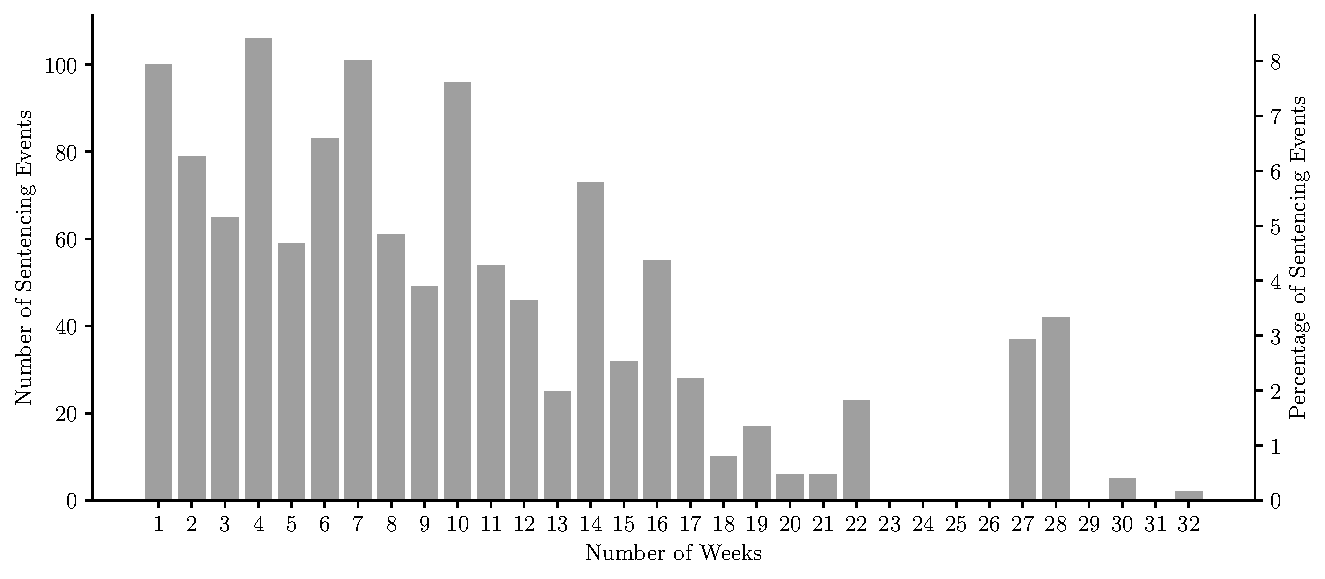
\includegraphics[scale=0.75]{Figures/Missing_Date_Histogram_of_Potential_Week_Histogram}
	\vspace{-2mm}
	\caption{A histogram of the number of weeks the judge visited the county in which the sentencing events missing the \emph{date} data field occurred.}
	\label{Figure_Missing_Date_Histogram_of_Potential_Week_Histogram}
\end{figure}

\noindent The data fields of the CSV file are as follows:

\vspace{-5mm}
\begin{enumerate}
	\itemsep-0.3em 
	\item An unnamed numeric identifier for the sentencing events. 
	\item date: Date of the sentence, ranging from 07/07/00 to 06/29/01; see Figure \ref{Figure_Hester_Data_Month_Histogram} in Appendix \ref{Sec:Appendix:Supplementary_Figures} for a histogram of the sentencing events across different months.
	\item county: The county where the sentence was decided. There are 46 counties; see Figure \ref{Figure_Hester_Data_County_Histogram} for a histogram of the sentencing counties.
	%
	\begin{figure}[H]
		\centering
		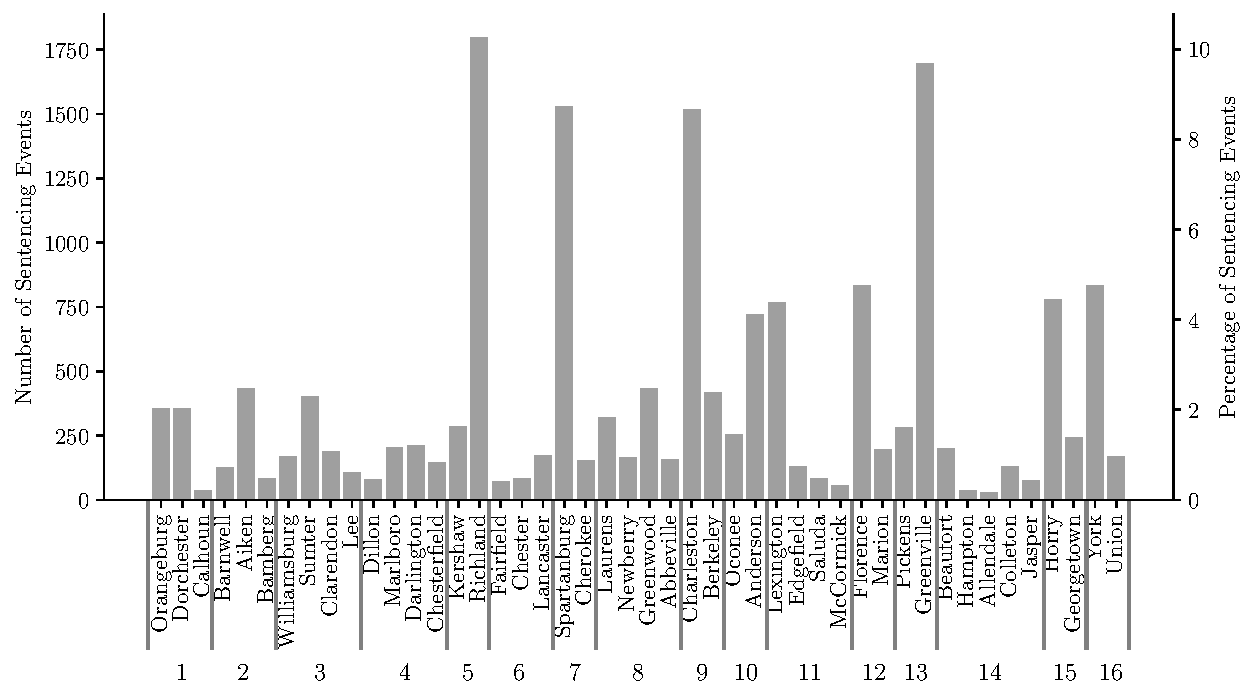
\includegraphics[scale=0.75]{Figures/County_Histogram}
		\vspace{-2mm}
		\caption{A histogram of the sentencing counties. The counties are grouped into 16 circuit courts. The number underneath each group indicates the corresponding circuit court.}
		\label{Figure_Hester_Data_County_Histogram}
	\end{figure}
	%
	\item circuit: The circuit court where the sentence was decided. There are 16 circuits: 1 to 16; see Figure \ref{Figure_Hester_Data_County_Histogram} and Table \ref{Table_Circuit_Court_Counties} (in Appendix \ref{Sec:Appendix:Supplementary_Tables}) for a list of the counties that belong to each circuit.
	\item judge: A numeric (identifier) for the judge who decided the sentence. There are 51 judges: 1 to 51; see Figure \ref{Figure_Hester_Data_Judge_Histogram} below for a histogram of the number of sentencing events observed for each judge.\footnote{Judge number 1 is a fictions judge. It is used for sentencing events for which the judge was not known; see the email from Rhys to Can and Larry on 05/14/2018 (Page 3 of the document Email3.pdf).} Figure \ref{Figure_Hester_Data_Judge_Missing_Date_Histogram} (in Appendix \ref{Sec:Appendix:Supplementary_Figures}) provides a histogram of the sentencing events missing the date data field for each judge. Only 2 of the 1551 sentencing events missing the date data field resulted in trial. Both sentencing events were undertaken by Juge 51.
	\item trial: Indicator (binary) variable indicating whether the case went to trial. Only $1.46\%$ of the cases went to trial; see Figure \ref{Figure_Hester_Data_Judge_Histogram} for a histogram of the number of cases undertaken by each judge and Figure \ref{Figure_Hester_Data_Judge_Trial_Percentage_Histogram} for the percentage of the sentencing events that resulted in a trial. Figures \ref{Figure_Hester_Data_Trial_Judge_Histogram} and \ref{Figure_Hester_Data_Judge_Plea_Histogram} (in Appendix \ref{Sec:Appendix:Supplementary_Figures}) provide a histogram of the number of trials and pleas undertaken by each judge, respectively. Figures \ref{Figure_Hester_Sentence_Length_Given_Trial_Histogram}-\ref{Figure_Hester_Sentence_Length_Given_Plea_Histogram} (in Appendix \ref{Sec:Appendix:Supplementary_Figures}) provide a histogram of the sentence lengths for the sentencing events that resulted in a trail and the sentencing events that resulted in a plea, respectively.
	%
	\begin{figure}[H]
		\centering
		\vspace{-2mm}
		\begin{minipage}{\textwidth}
			\vspace{-0mm}
			\centering
			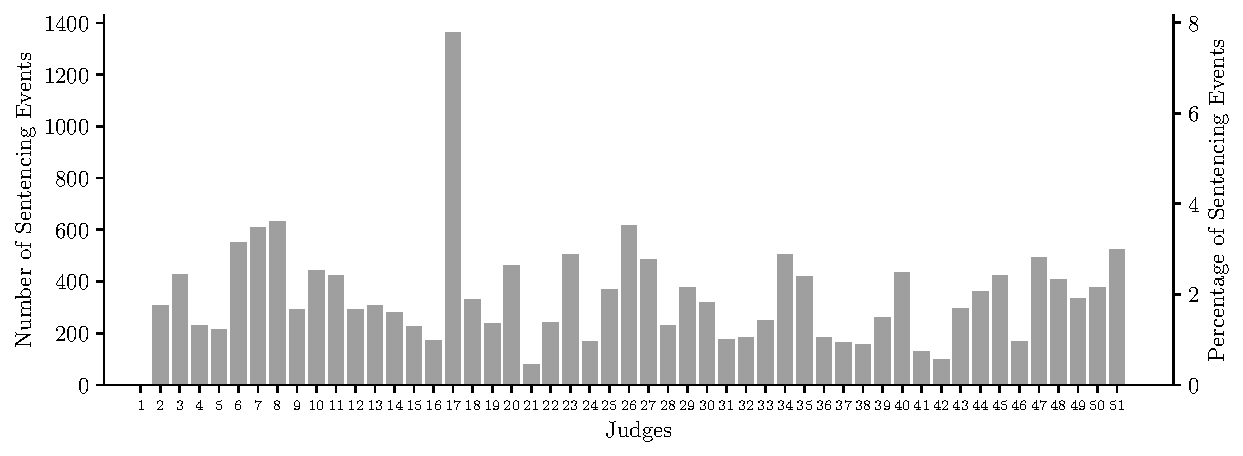
\includegraphics[scale=0.75]{Figures/Judge_Histogram}
			\vspace{-4mm}
			\caption{A histogram of the sentencing judges.}
			\label{Figure_Hester_Data_Judge_Histogram}
		\end{minipage}
		\begin{minipage}{\textwidth}
			\vspace{-0.5mm}
			\centering
			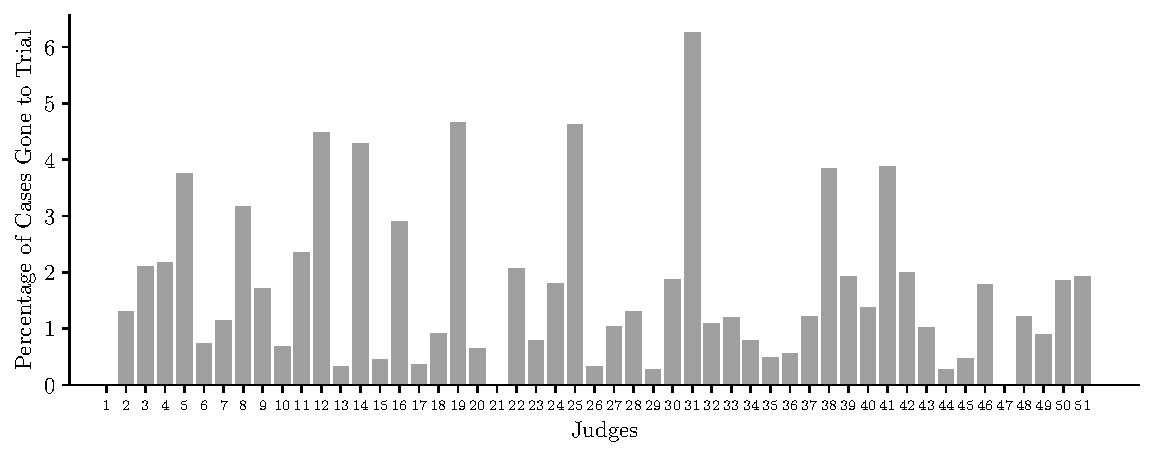
\includegraphics[scale=0.75]{Figures/Judge_Trial_Percentage_Histogram}
			\vspace{-4mm}
			\caption{Percentage of sentencing events (for each judge) that resulted in trial.}
			\label{Figure_Hester_Data_Judge_Trial_Percentage_Histogram}
		\end{minipage}
	\end{figure}
	%
	\item incarc: Indicator (binary) variable indicating whether the sentence includes incarceration. In aggregate, about $37.41\%$ of the cases resulted in incarceration. To be more specific, about $36.55\%$ of the cases that ended with a plea and about $95.74\%$ of the cases that ended with a trial resulted in incarceration. The remaining sentencing events have a sentence length of zero.
	\item statute: The (code of) law that the offender broke. For example, 56-05-0750(B)(1). There are 253 distinct entries; see Figure \ref{Figure_Statute_Histogram} in Appendix \ref{Sec:Appendix:Supplementary_Figures} for a histogram.\footnote{For a detailed description of South Carolina code of laws, please see \url{https://law.justia.com/codes/south-carolina} (accessed on October 17th, 2020). For example, a detailed description of 56-05-0750 is provided in \url{https://law.justia.com/codes/south-carolina/2019/title-56/chapter-5/section-56-5-750} (accessed on October 17th, 2020).}
	\label{CSV_File_Statute_Item}
	\item offdescr: A description of the offense. For example, "Failure to Stop for a Blue Light, No Injury or Death - 1st Offence".
	\item counts: There are 29 distinct values, ranging between 0 and 60; see Figure \ref{Figure_Hester_Data_Counts_Histogram} in Appendix \ref{Sec:Appendix:Supplementary_Figures} for a histogram.
	\item statute\_first: The description of the first offense of the offender. For example, 56-05-0750(B)(1). This data field is identical to statute data field (numbered \ref{CSV_File_Statute_Item} above).
	\item offdescr\_first: A description of the first offense. For example, "Pointing and Presenting Firearms at a Person".
	\item sgc\_offcode: 286 distinct numeric values between 4 and 2878; see Figure \ref{Figure_Hester_Data_sgc_offcode_Histogram} in Appendix \ref{Sec:Appendix:Supplementary_Figures} for a histogram. The set of sgc\_offcode values can be partitioned into four subsets: $\mathcal{C}_1$, $\mathcal{C}_2$, $\mathcal{C}_3$, and $\mathcal{C}_4$; see \citet{Hester_Hartman_2017} for the partitions.\footnote{See the code provided on \url{https://tkhartman.netlify.app} (accessed on October 17th, 2020) for \citet{Hester_Hartman_2017}.} Each partition is associated with a unique minimum sentence multiplier, i.e., the fraction of the sentence that has to pass before the defendant is eligible for parole. Let $c$ denote the sgc\_offcode code for a sentencing event. Then, the minimum sentence multiplier (for this sentencing events) is
		\begin{align*}
		m(c) \,=\, \left \{\!\! \begin{array}{ll}
		1.00 & \text{if } c \in \mathcal{C}_1, \\
		0.85 & \text{if } c \in \mathcal{C}_2, \\
		0.33 & \text{if } c \in \mathcal{C}_3, \\
		0.25 & \text{if } c \in \mathcal{C}_4. \\
		\end{array} \right.
		\end{align*}
		Also, define the sets
		\begin{align*}
		&\mathcal{A}_1 = \{267, 383, 2362\},\\
		&\mathcal{A}_2 = \{454, 2360, 2362\},\\
		&\mathcal{A}_3 = \{79, 90, 113, 114, 139, 217, 280, 283, 312, 368, 387, 388, 389, 392, 395, 402, 457, 2356, 2359\}, \\ &\mathcal{A}_4 = \{116, 148, 281, 284, 349, 370, 452, 456, 2417\},
		\end{align*}
		where $\mathcal{A}_i \subset \mathcal{C}_i$ for $i=1,2,3,4$. According to \citet{Hester_Hartman_2017}, a mandatory minimum sentence is imposed if $c \,\in\, \mathcal{A}_1 \cup \mathcal{A}_2 \cup \mathcal{A}_3 \cup \mathcal{A}_4$.
	\vspace{1mm}
	\item[-] The next ten data fields indicate the crime type; see Table \ref{Table_Sentencing_Crime_Type_Data_Fields} below for a list of these data fields and Figure \ref{Figure_Hester_Data_Crime_Type_Histogram} in Appendix \ref{Sec:Appendix:Supplementary_Figures} for a histogram of the crime types.
	%
	\vspace{1mm}
	\begin{table}[H]
		\centering
		\caption{The ten data fields that indicate the crime type and their definition.} 
		\vspace{-2mm}
		\setlength\tabcolsep{8pt} % default value: 6pt
		{\footnotesize
			\hspace{10mm}
			\begin{tabular}{L{20mm}L{115mm}}
				\toprule
				Data Field & Description \\
				\midrule
				%\rowgroup{Consumer Surplus} \\
				14. of\_hom & Indicator (binary) variable for the offense type being homicide \\
				15. of\_rape & Indicator (binary) variable for the offense type being rape \\		
				16. of\_rob & Indicator (binary) variable for the offense type being robbery \\
				17. of\_asslt & Indicator (binary) variable for the offense type being assault \\
				18. of\_burg & Indicator (binary) variable for the offense type being burglary \\
				19. of\_dstrb & Indicator (binary) variable for the offense type being drug distribution \\
				20. of\_possn & Indicator (binary) variable for the offense type being drug possession\\
				21. of\_theft & Indicator (binary) variable for the offense type being theft \\
				22. of\_fraud & Indicator (binary) variable for the offense type being fraud \\
				23. of\_other & Indicator (binary) variable for the offense type belonging to the category "other" \\				
				\bottomrule
			\end{tabular}
		}
		\label{Table_Sentencing_Crime_Type_Data_Fields}
	\end{table}
	\vspace{-2mm}
	%
	\skipitems{10}
	\item offtypeLibHyp: Categorical offense type. The categories: Property, Violent, Other, and Drug. Figure \ref{Figure_Hester_Data_Categorical_Offense_Type_Histogram} in Appendix \ref{Sec:Appendix:Supplementary_Figures} provides a histogram of the categorical offense types and Figure \ref{Figure_Hester_Data_offtypeLibHyp} in Appendix \ref{Sec:Appendix:Supplementary_Figures} provides a histogram of the crime types associated with (observed alongside) each categorical offense type.
	\item offser: Offense seriousness. There are 8 categories: 1 to 8. The categories in the increasing order of seriousness are as follows: 1-Misdemeanours, 2-Class F Felonies, 3- Class E Felonies, 4-Class D Felonies, 5-Class A Felonies, 6-Class B Felonies, 7-Class C Felonies. The unclassified felonies are grouped into category 8. Figure \ref{Figure_Hester_Data_Offense_Seriousness_Histogram} in Appendix \ref{Sec:Appendix:Supplementary_Figures} provides a histogram of the offense seriousness.
	\item ccpnts: Numeric values between 1 and 68; see Figure \ref{Figure_Hester_Data_ccpnts_Histogram} in Appendix \ref{Sec:Appendix:Supplementary_Figures} for a histogram.
	\item ccpts99: Commitment score. Numeric values between 1 and 12 in the increasing order of seriousness. This is an alternative measure of offense seriousness. The mean and standard deviations are 1.9 and 1.8, respectively. Figure \ref{Figure_Hester_Data_ccpts99_Histogram} in Appendix \ref{Sec:Appendix:Supplementary_Figures} provides a histogram.
	\item crimhist: Criminal history of the defendant. The five categories in the increasing order of appearance are as follows: extensive, voluminous, moderate, minimal, and none; see Figure \ref{Figure_Hester_Data_Crime_History_Histogram} for a histogram.	
	%
	\begin{figure}[h!]
		\centering
		\vspace{1mm}
		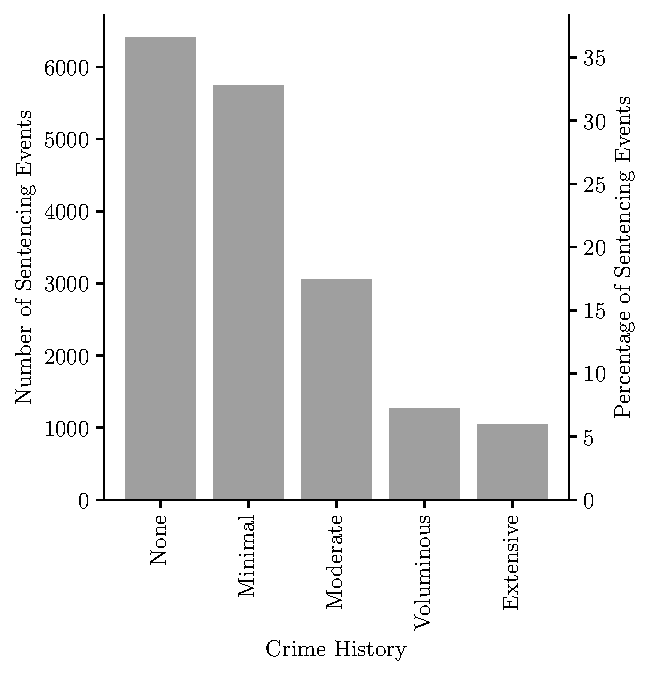
\includegraphics[scale=0.75]{Figures/Crime_History_Histogram}
		\vspace{-2mm}
		\caption{A histogram of the crime histories.}
		\label{Figure_Hester_Data_Crime_History_Histogram}
		\vspace{-2mm}
	\end{figure}
	%
	\item ppoints: Numeric values between 0 and 1014; see Figure \ref{Figure_Hester_Data_PPoints_Histogram} in Appendix \ref{Sec:Appendix:Supplementary_Figures} for a histogram of ppoints.
	\vspace{-2mm}
	\item male: Indicator (binary) variable indicating whether the defendant is male; $83.42\%$ of the defendants are male.		
	\item age: Age of the defendant at sentencing. There are 65 distinct values between 15 and 81. The mean and the standard deviation are 31.3 and 10.1, respectively; see Figure \ref{Figure_Hester_Data_Age_Histogram} in Appendix \ref{Sec:Appendix:Supplementary_Figures} for a histogram.
	\item black: Indicator (binary) variable indicating whether the defendant is black. About $61.97\%$ of the defendants are black. We do not have any other information on the race of the defendant.	
	\item sentence: The length of the sentence (in months).\footnote{Rhys refers to this as the initial sentence; see the email from Rhys to Can and Larry on 05/08/2018 (Page 2 of the document Email3.pdf).} There are 237 distinct values between 0 and 11988 (corresponds to between 0 and 99 years); see Figure \ref{Figure_Hester_Sentence_Length_Histogram} in Appendix \ref{Sec:Appendix:Supplementary_Figures} for a histogram.
\end{enumerate}

\vspace{-4mm}
\subsection{Stata File} 
\label{Sec:Data_Description:STATA}
Next, we describe the data fields of the STATA file. We only describe the two data fields that are specific to the STATA file. The remaining data fields have already been discussed above.
\vspace{-4mm}
\begin{enumerate}
	\itemsep-0.3em 
	\item expmin: The expected minimum sentence. There are 313 distinct values between 0 and 470 (corresponding to between 0 and 39 years); 28 sentencing events are missing this information. This corresponds to 0.15\% of the sentencing events. Figure \ref{Figure_Hester_ExpMin_Histogram} in Appendix \ref{Sec:Appendix:Supplementary_Figures} provides a histogram of the expected minimum sentences. The expected minimum sentence (reported in the STATA file) is calculated as follows:\footnote{See the code provided on \url{https://tkhartman.netlify.app} (accessed on October 17th, 2020) for \citet{Hester_Hartman_2017}.} As discussed above, the set of sgc\_offcode values is partitioned into four subsets: $\mathcal{C}_1$, $\mathcal{C}_2$, $\mathcal{C}_3$, and $\mathcal{C}_4$; see \citet{Hester_Hartman_2017} for the partitions. Let $s$ denote the sentence length in months, $c$ denote the sgc\_offcode, and
		\begin{align*}
			m(c) \,=\, \left \{\!\! \begin{array}{ll}
			1.00 & \text{if } c \in \mathcal{C}_1, \\
			0.85 & \text{if } c \in \mathcal{C}_2, \\
			0.33 & \text{if } c \in \mathcal{C}_3, \\
			0.25 & \text{if } c \in \mathcal{C}_4, \\
			\end{array} \right.
		\end{align*}
		denote the expected minimum sentence multiplier, i.e., the fraction of the sentence that has to pass before the defendant is eligible for parole. Then,\footnote{A mandatory minimum sentence is imposed for a subset of sgc\_offcode values; See Section \ref{Sec:Data_Description:CSV} for details.}
		\begin{align}
		\text{Expected Minimum Sentence}\,(s,c) \,=\, \min \big\{ \big\lceil m(c) s \big\rceil ,720 \big\}.
		\label{Equation_Expected_Minimum_Sentence}
		\end{align}
		%As an aside, according to \citet{Hester_Hartman_2017}, a mandatory minimum sentence is imposed if 
		%\begin{align*}
		%	c \,\in\, \big\{&79,90,113,116,114,139,148,217,267,280,281,283,284,312,349,368,370,383,\\
		%	&387,388,389,392,395,402,452,454,456,457,2356,2359,2360,231,2362,2417 \big\}.
		%\end{align*}
	\item jud\_no: An identifier for the judges. There are 50 judges: Numbers 1 to 54 excluding 16, 42, 44, and 49.\footnote{According to Rhys, judges 16, 42, 44, and 49 were dropped from the dataset probably either because they had retired (but still hearing some cases) or they had some special appointment or caseload jurisdiction; see the email from Rhys to Can and Larry on 05/14/2018 (Page 3 of the document Email3.pdf).} A small fraction ($0.88\%$) of the sentencing events are missing the jud\_no data field. Consider the following mapping from the numeric identifiers used in the judge data field of the CSV file to the numeric identifiers used in the jud\_no data field of the STATA file: Each non-fictitious judge number (judges 2 to 51) in the CSV file is mapped to the judge number in the STATA file that has the highest number of sentencing events in common with the judge in the CSV file. Under this mapping, the judge identifiers match for 98.79\% of the sentencing events. Of the remaining 1.21\% sentencing events, 1.13\% are cases in which either the judge data field entry is 1 (the fictitious judge) or the jud\_no data field is empty. In the remaining 0.08\% of the sentencing events (15 events), the judge identifiers in the two files do not match. However, this is a small fraction of the sentencing events.
\end{enumerate}

\section{Master Calendar}
\label{Sec:Master_Calendar_Description}

The master calendar describes the schedule of the judges between July 2000 and June 2001; see Figure \ref{Figure_Master_Calendar_0} for a snapshot of the master calendar for November. The schedule of each month is described in a table, where the first column indicates the judge names. The remaining columns corresponds to the weeks in that month. We \emph{assume} judges do not work on the weekends. The number written on top of each column indicates the date of the Monday of that week. For example, the first column in Figure \ref{Figure_Master_Calendar_0} corresponds to the week of November 6th. Each row describes the schedule of one judge.
%
\begin{figure}[H]
	\centering
	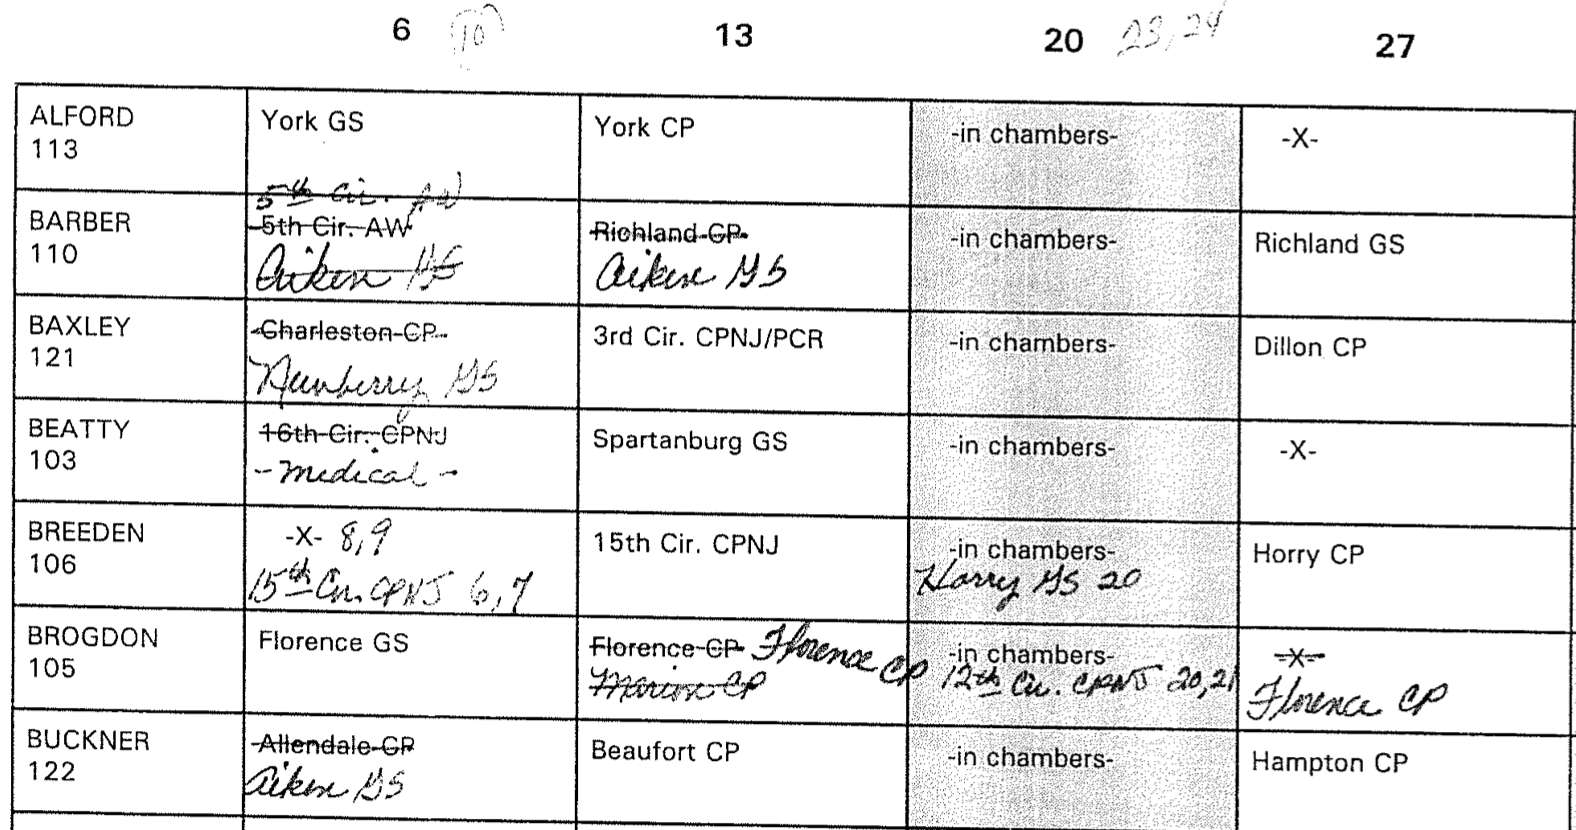
\includegraphics[scale=0.4]{Figures/Fig1}
	\caption{A snapshot of the November Calendar.}
	\label{Figure_Master_Calendar_0}
\end{figure} 

In what follows, we assume the master calendar is cleaned as described in Appendix \ref{Sec:Appendix:Data_Cleaning}. Figure \ref{Figure_Assignment_Histogram} provides a histogram of the different types of (judge) assignments on the master calendar. In other words, it depicts the number of judge-week combinations that have an assignment that belongs to one of the following ten categories: county, circuit court, in chamber, vacation, official leave, sick, medical, orientation school, family death, and military. For example, the first bar indicates that 1769 judge-week combinations have a county assignment. This need not be the only assignment of this judge-week combination. When there are multiple assignments for a judge-week combination, each of those is separately accounted for in Figure \ref{Figure_Assignment_Histogram}.

Most assignments on the master calendar end with an acronym, e.g., Horry GS. We refer to these acronyms as assignment types. Table \ref{Table_Assignment_Type_Meaning} provides a list of the acronyms and their meanings. Figure \ref{Figure_Assignment_Type_Histogram} provides a histogram of the acronyms. In other words, it depicts the number of judge-week combinations that have an assignment of a specific type. For example, the first bar indicates that 989 judge-week combinations have an assignment that ends with GS. 

Figure \ref{Figure_Assignment_Type_Sentencing_Event_Histogram} depicts the frequency of the assignment types based on the sentencing dataset. Figure \ref{Figure_Assignment_Type_Sentencing_Event_Histogram} is generated as follows: First, we create a list of the sentencing events undertaken by Judges $2,\ldots,51$ that have a date. Then, for each sentencing event on the list, we proceed as follows:
\begin{enumerate}
	\vspace{-3mm}
	\item We read the judge number, the week, and the county corresponding to each sentencing event (from the sentencing dataset). For example, Judge 2 on the Week of January 8 in Chester.\footnote{The subsequent analysis in this section shows that there are some inconsistencies between the master calendar and the sentencing dataset. If we use the sentence date (to generate Figure \ref{Figure_Assignment_Type_Sentencing_Event_Histogram}), we will run into a problem for some sentencing events, e.g., the sentencing events in Table \ref{Table_Mater_Calendar_Problematic_Cases_Detailed_Category_i}. Therefore, we make a weaker assumption and use the sentence week (as opposed to sentence date).}
	\vspace{-2mm}
	\item We look for the judge's assignment for this week on the master calendar and report the type of the assignment in the figure. We sometimes observe multiple assignments in a week. For example, Judge 2 had the following assignments in the week of January 8: 2nd Cir. CPNJ 8, Chester GS 9,10,11, and Lancaster 12. In this case, the assignment in Chester county is the one we are interested in, because that is where the sentencing event of interest occurred. Thus, we use this assignment (and its type, i.e., GS) to record the sentencing event in the figure. For 4.12\% of the sentencing events (without a date), we cannot find the county assignment we are interested in due to inconsistencies between the master calendar and the sentencing dataset; see Section \ref{Sec:Master_Calendar:Further_Analysis_of_Some_Assignments} for a detailed description of the judge-week combinations in which these sentencing events occurred. Nonetheless, the analysis summarized in Figure \ref{Figure_Assignment_Type_Sentencing_Event_Histogram} is still useful for our capacity calculations below.
\end{enumerate}
\vspace{-3mm}
We repeat this procedure for all sentencing events and count the number of assignment types. Finally, we plot the histogram in Figure \ref{Figure_Assignment_Type_Sentencing_Event_Histogram}. 

For each judge, the percentage of weeks with a GS (CP) assignment on the master calendar is depicted in Figure \ref{Figure_Judge_Schedule_GS_Percentage_Histogram} (\ref{Figure_Judge_Schedule_CP_Percentage_Histogram}). Figures \ref{Figure_Judge_Schedule_GS_Percentage_Histogram}-\ref{Figure_Judge_Schedule_CP_Percentage_Histogram} jointly show that GS and CP assignments are the most common assignments for the judges. Figure \ref{Figure_Judge_Schedule_GS_CP_Percentage_Histogram} shows the overlap, i.e., the percentage of weeks (with an assignment) in which the judge has at least one assignment of type GS and at least one assignment of type CP. It shows that it is not common for a judge to have both GS and CP assignments in a week.

\begin{figure}[H]
	\centering
	\hspace*{-8mm}
	\begin{minipage}{.45\textwidth}
		\centering
		\hspace*{-10mm}
		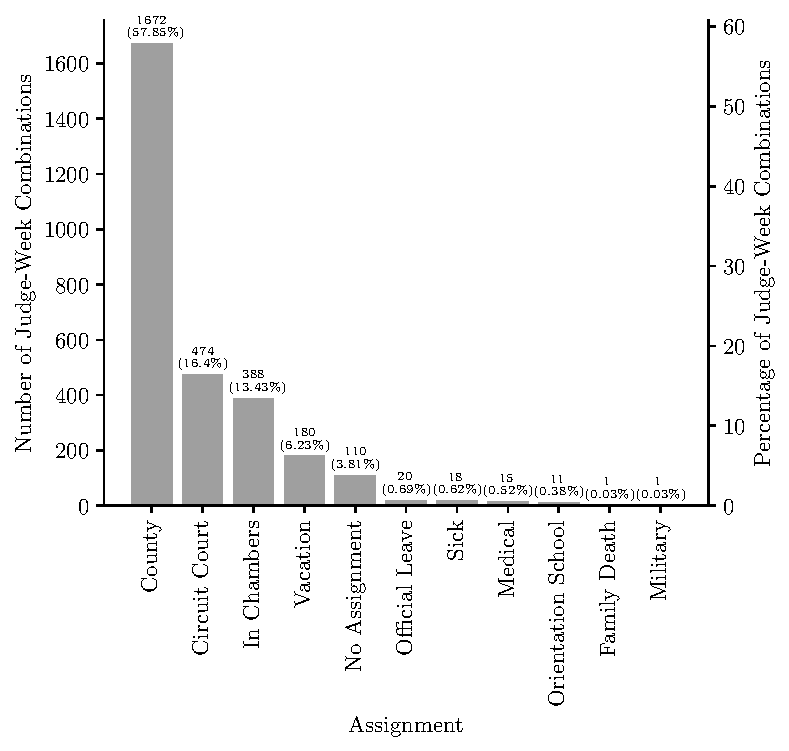
\includegraphics[scale=0.67]{Figures/Type_of_Assignment_Histogram}
		\vspace*{-7mm}
		\caption{A histogram of the assignments observed for a judge-week combination in the master calendar.}
		\label{Figure_Assignment_Histogram}
	\end{minipage}
	\hspace{5mm}
	\begin{minipage}{0.45\textwidth}
		\centering
		\vspace*{0mm}
		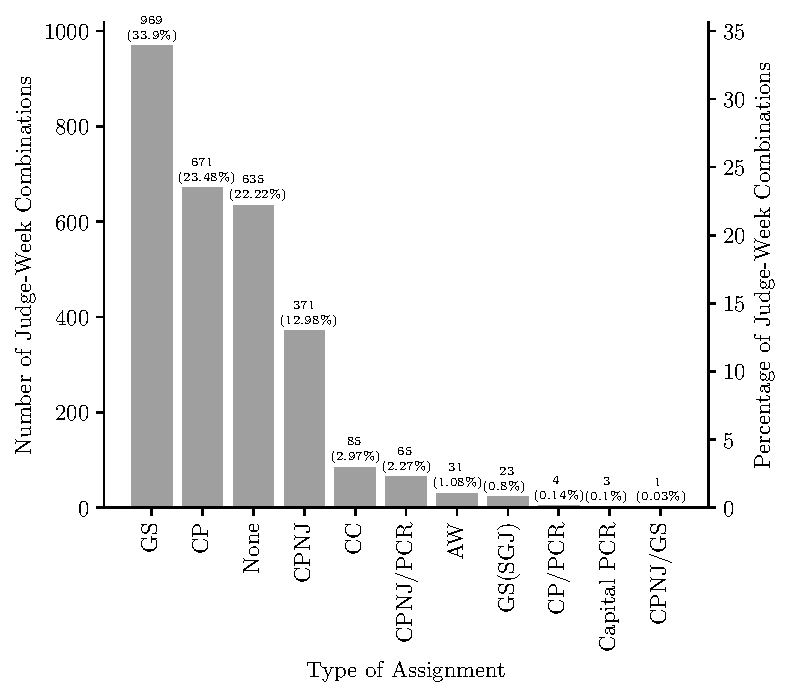
\includegraphics[scale=0.67]{Figures/Type_of_Court_Assignment_Histogram}
		\vspace*{-1mm}
		\caption{A histogram of the assignment types observed for a judge-week combination in the master calendar.}
		\label{Figure_Assignment_Type_Histogram}
	\end{minipage}
\end{figure}

\begin{table}[H]
	\centering
	\caption{Assignment Type Acronyms and their meanings.} 
	\vspace{0mm}
	\setlength\tabcolsep{8pt} % default value: 6pt
	{\footnotesize
		\begin{tabular}{L{20mm}L{50mm}}
			\toprule
			Acronym & Meaning  \\
			\midrule
			%\rowgroup{Consumer Surplus} \\
			GS & General Session \\
			CC & Circuit Court \\
			SGJ & State Grand Jury \\
			CP & Common Pleas \\
			CPNJ & Common Pleas Non-Jury \\
			PCR & Post Conviction Relief  \\
			Capital PCR & Capital Post Conviction Relief  \\
			AW & Administrative Week \\
			\bottomrule
		\end{tabular}
	}
	\label{Table_Assignment_Type_Meaning}
\end{table} 

\begin{figure}[H]
	\centering
	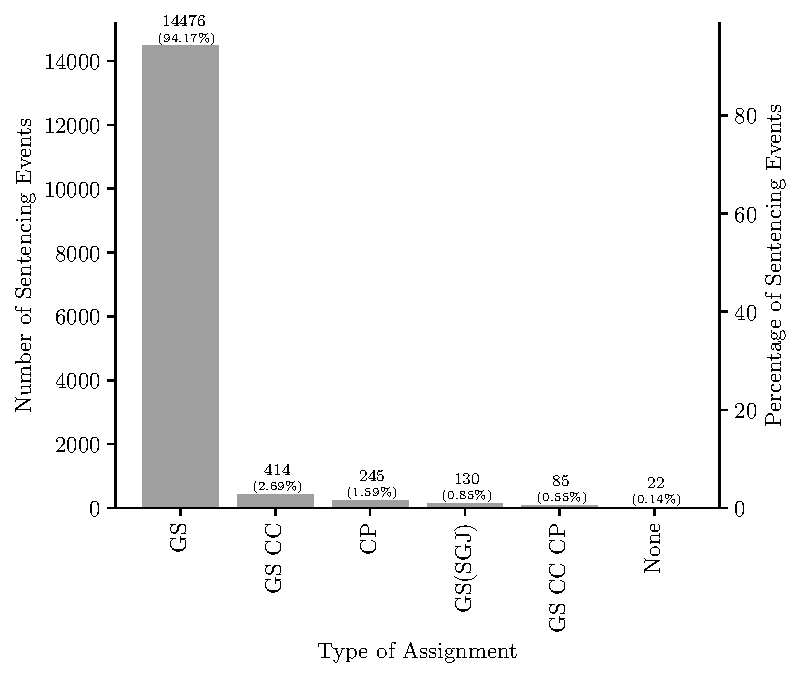
\includegraphics[scale=0.75]{Figures/Type_of_Court_Assignment_Sentencing_Event_Histogram}
	\caption{A histogram of the type of the assignment (on the master calendar) during which the sentencing events occurred.}
	\label{Figure_Assignment_Type_Sentencing_Event_Histogram}
\end{figure}

\begin{remark}
	We should probably only keep the following assignments (in the master calendar):
	\begin{enumerate}
		\vspace{-2mm}
		\item All county assignments of type GS 
		\item All county assignments of type GS CC, GS CC CP, and GS(SGJ) in which a sentencing event occurred; see Figure \ref{Figure_Assignment_Type_Sentencing_Event_Histogram}. Note, however, in these weeks the judge may be splitting his time between GS (criminal cases) and other assignment types (e.g., civil cases). Therefore, we do not include these assignments in the estimation of $\mu_p$, the plea service rate.
		\item The CP county assignments that account for the 245 sentencing events in the CP bar of Figure \ref{Figure_Assignment_Type_Sentencing_Event_Histogram}. Since the sentencing dataset only includes the criminal cases and a CP session is for civil cases, we believe in these CP county assignments, the GS acronym was omitted. Even then, because the judge may be splitting his capacity between GS and CP, we do not include these assignments in the estimation of $\mu_p$, the plea service rate.
		\item The one (hand-written) assignment without an acronym in front of it that accounts for the 22 sentencing events in the None bar of Figure \ref{Figure_Assignment_Type_Sentencing_Event_Histogram}. Since the sentencing dataset only includes the criminal cases, we believe in this assignment, the GS acronym was omitted. Nevertheless, we do not include this assignment in the estimation of $\mu_p$, the plea service rate.
	\end{enumerate}
\end{remark}

\begin{figure}[H]
	\centering
	\begin{minipage}{\textwidth}
		\vspace{-16mm}
		\centering
		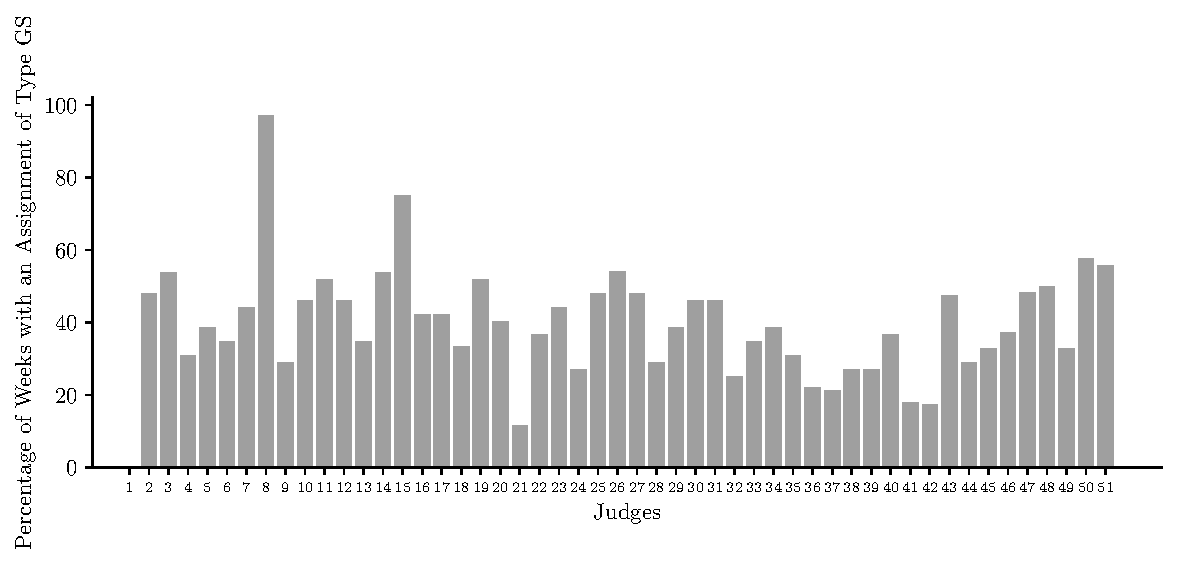
\includegraphics[scale=0.75]{Figures/Judge_Schedule_GS_Percentage_Histogram}
		\vspace{-3mm}
		\caption{The percentage of weeks (with an assignment) in which the judge has at least one assignment of type GS.}
		\label{Figure_Judge_Schedule_GS_Percentage_Histogram}
	\end{minipage}
	\begin{minipage}{\textwidth}
		\centering
		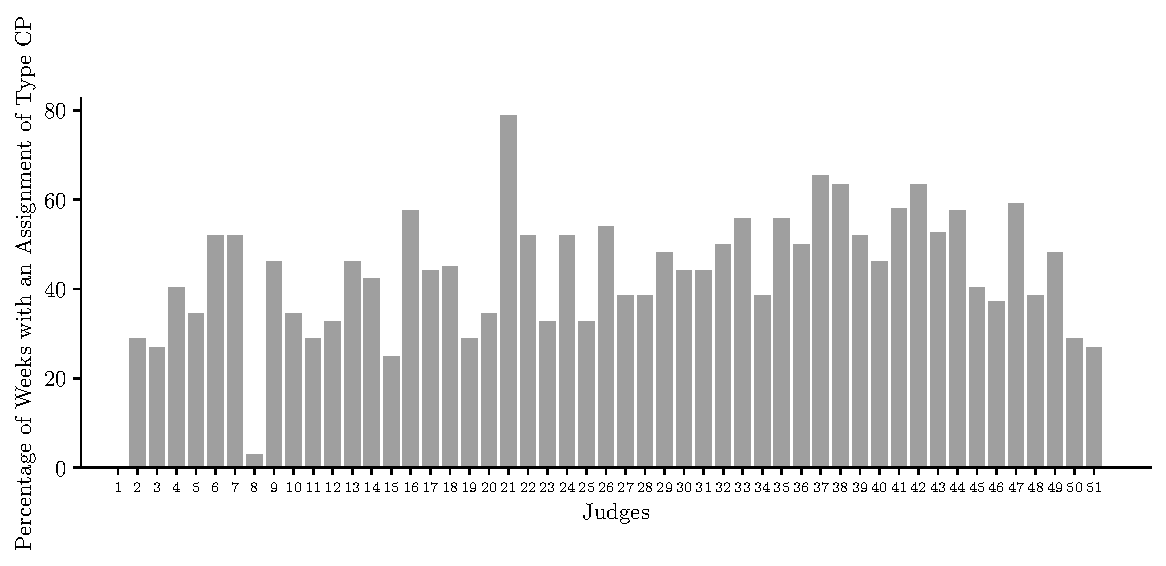
\includegraphics[scale=0.75]{Figures/Judge_Schedule_CP_Percentage_Histogram}
		\vspace{-3mm}
		\caption{The percentage of weeks (with an assignment) in which the judge has at least one assignment of type CP.}
		\label{Figure_Judge_Schedule_CP_Percentage_Histogram}
	\end{minipage}
	\begin{minipage}{\textwidth}
		\centering
		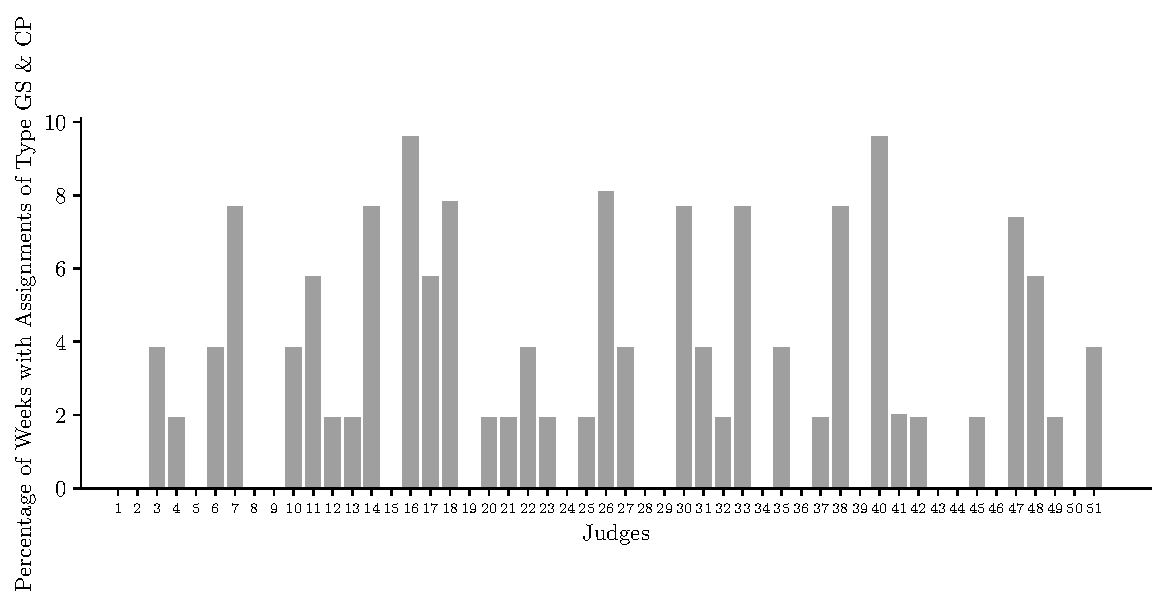
\includegraphics[scale=0.75]{Figures/Judge_Schedule_GS_CP_Percentage_Histogram}
		\vspace{-3mm}
		\caption{The percentage of weeks (with an assignment) in which the judge has at least one assignment of type GS and at least one assignment of type CP.}
		\label{Figure_Judge_Schedule_GS_CP_Percentage_Histogram}
	\end{minipage}
\end{figure}

\subsection{Interpreting the Master Calendar}
\label{Sec:Master_Calendar:Interpreting_Master_Calendar}

Consider a judge on a specific week. We group the judge-week combinations into four categories, depending on the number of assignment the judge has during that week, as follows: i) None (blank), ii) a single assignment, iii) two assignments, and (iv) more than two assignments.

\begin{figure}[h!]
	\centering
	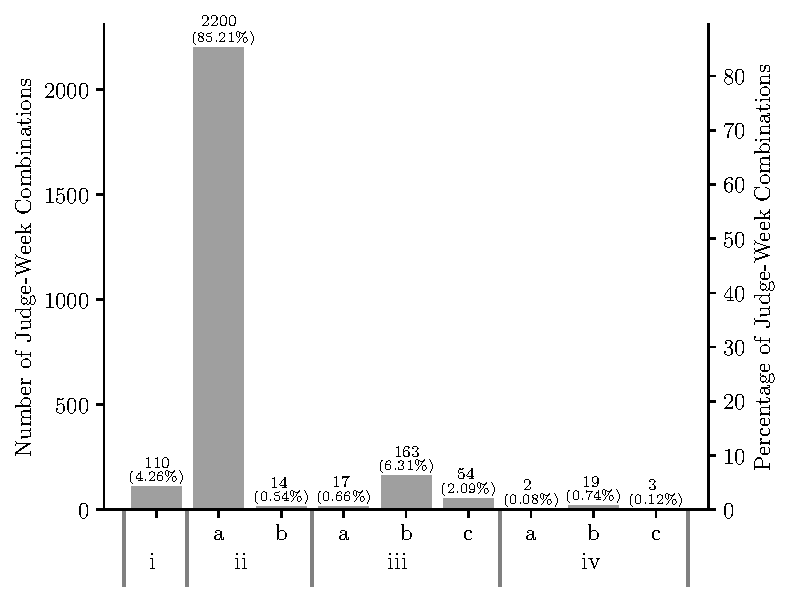
\includegraphics[scale=0.75]{Figures/Simultaneous_Assignment_Count_Histogram}
	\caption{A histogram of the assignment categories observed for a judge-week combination in the master calendar.}
	\label{Figure_Simultaneous_Assignment_Count_Histogram}
\end{figure}
	
Figure \ref{Figure_Simultaneous_Assignment_Count_Histogram} provides a histogram of the assignment categories observed for a judge-week combination in the master calendar. We compare these assignments in the master calendar with the sentencing events for the judge recorded in the sentencing dataset. Next, we discuss our interpretation  of each assignment category with examples. We have a total of 2556 judge-week combinations.

\vspace{-3mm}
\paragraph{i) No Assignments (110 judge-week combinations).}
\label{Category_i}
As will be discussed in Section \ref{Sec:Master_Calendar:Further_Analysis_of_Some_Assignments}, we do not observe any sentencing events for 101 of the 110 judge-week combinations in this category. The remaining 9 judge-week combinations are listed in Table \ref{Table_Mater_Calendar_Problematic_Cases_Detailed_Category_i} in Section \ref{Sec:Master_Calendar:Further_Analysis_of_Some_Assignments:Category_i}.

\begin{figure}[H]
	\centering
	\vspace{-0mm}
	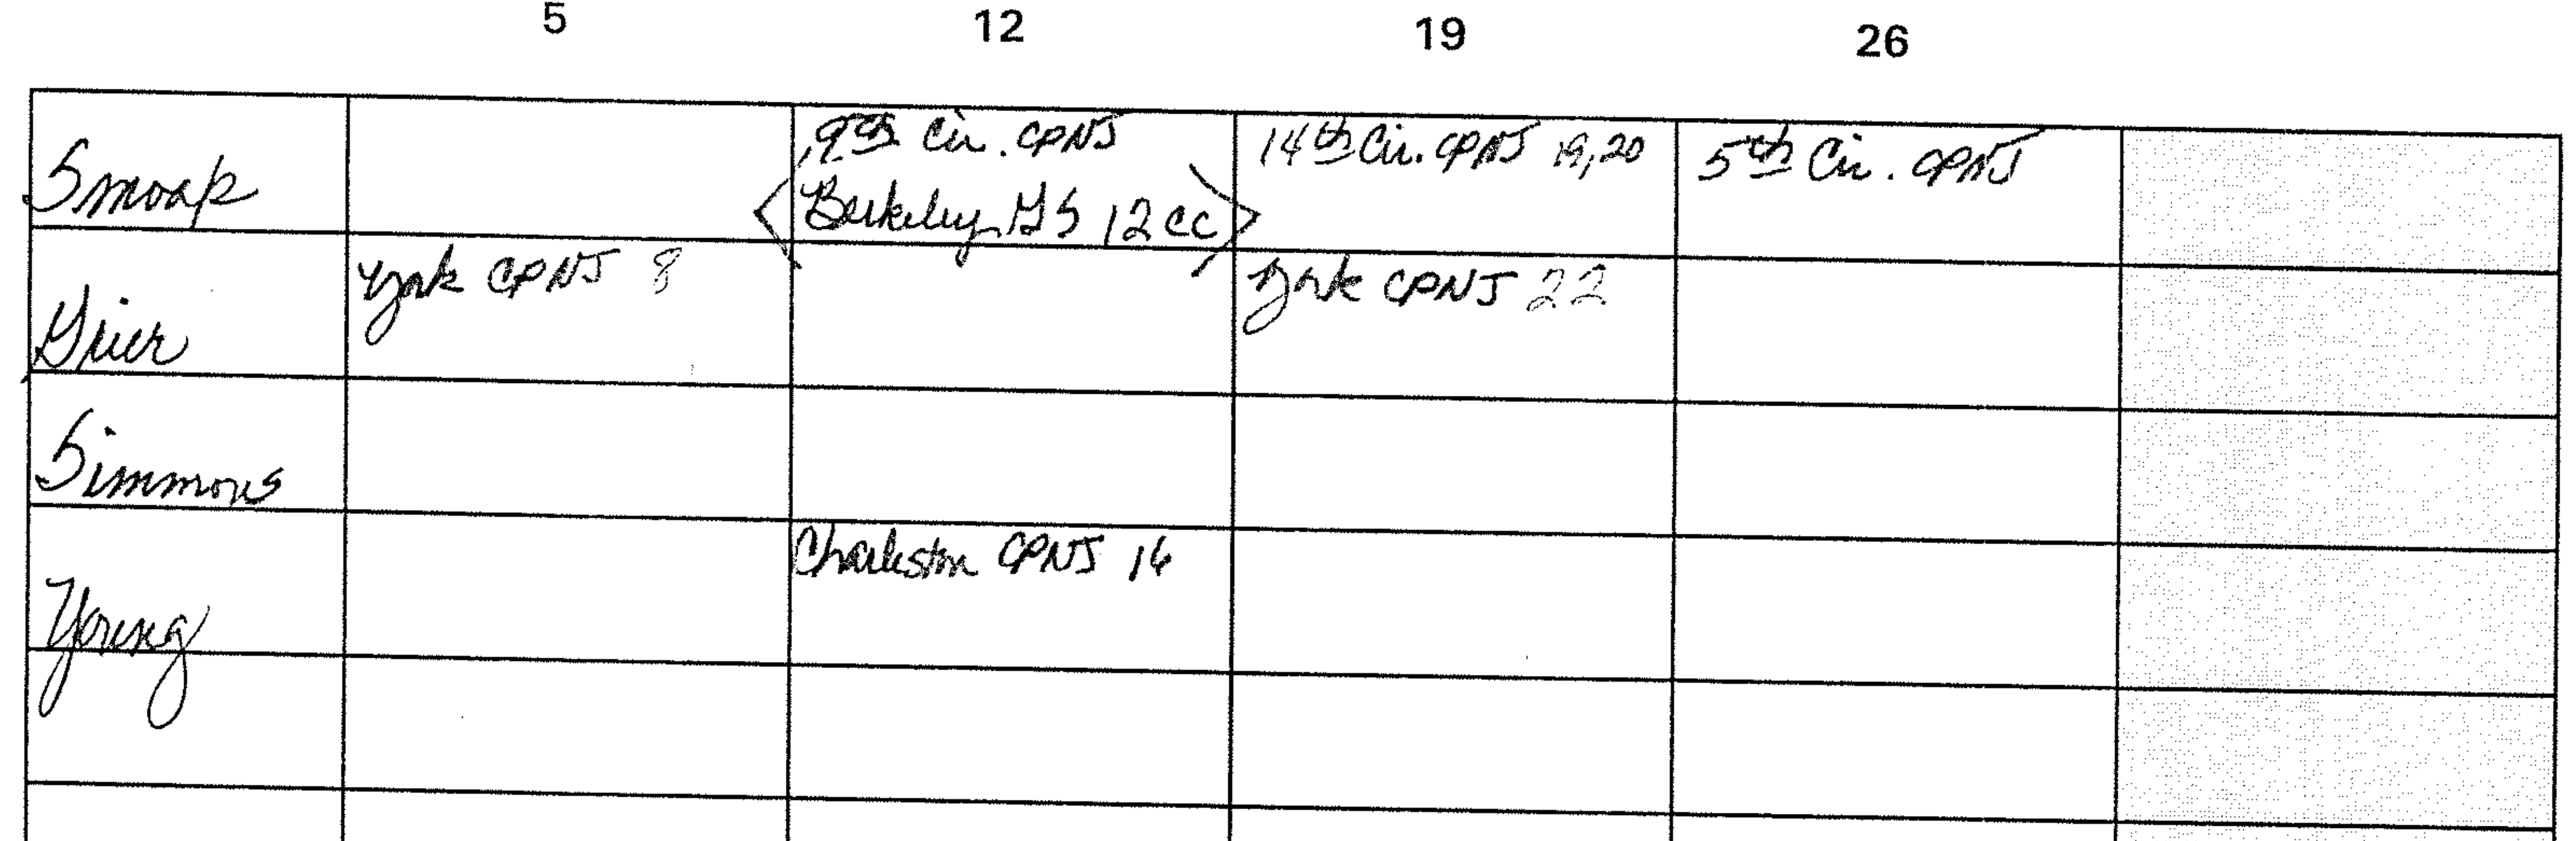
\includegraphics[scale=0.097]{Figures/Fig2}
	\caption{A snapshot of the March Calendar.}
	\label{Figure_Master_Calendar_1}
\end{figure}

\vspace{-3mm}
\paragraph{ii) A Single Assignment (2196 judge-week combinations).} 
\label{Category_ii}
A single assignment occurs in two ways as discussed next:
	\begin{itemize}
		\vspace{-2mm}
		\item[(a)] \emph{No date is indicated (2200 judge-week combinations).} For example, Judge Alford's assignment (on the master calendar) for the week of November 6th is York GS; see Figure \ref{Figure_Master_Calendar_0}. As will be discussed in Section \ref{Sec:Master_Calendar:Further_Analysis_of_Some_Assignments}, we only observe sentencing events in the county stated on the master calendar for 1872 of the 2200 ($85.1\%$) judge-week combinations in this category. In other words, there are no inconsistencies between the master calendar and the sentencing dataset for 1872 of the 2200 judge-week combinations. The remaining 328 judge-week combinations are listed in Table \ref{Table_Mater_Calendar_Problematic_Cases_Detailed_Category_iia} and involve contradictory sentencing locations based on the sentencing dataset.
		\vspace{-2mm}
		\item[(b)] \emph{Specific dates are indicated (14 judge-week combinations).} For example, Judge Smoak's assignment (on the master calendar) in the week of March 19th is 14th Cir. CPNJ 19,20; see Figure \ref{Figure_Master_Calendar_1}. As will be discussed in Section \ref{Sec:Master_Calendar:Further_Analysis_of_Some_Assignments}, we observe sentencing events only in the county stated on the master calendar and on the days stated on the master calendar for 10 of the 14 ($71.4\%$) judge-week combinations in this category. In other words, there are no inconsistencies between the master calendar and the sentencing dataset for 10 of these 14 judge-week combinations. The remaining 4 judge-week combinations are listed in Table \ref{Table_Mater_Calendar_Problematic_Cases_Detailed_Category_iib} and involve contradictory sentencing locations based on the sentencing dataset.
	\end{itemize}

\begin{figure}[ht]
	\centering
	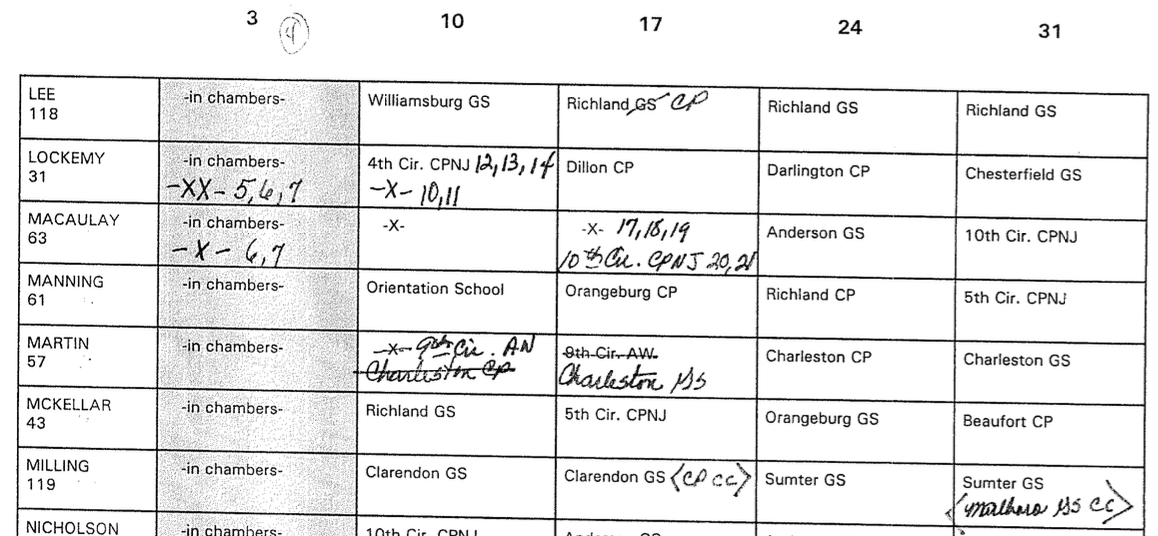
\includegraphics[scale=0.6]{Figures/Fig4}
	\caption{Another snapshot of the July Calendar.}
	\label{Figure_Master_Calendar_4}
\end{figure} 

\begin{figure}
	\centering
	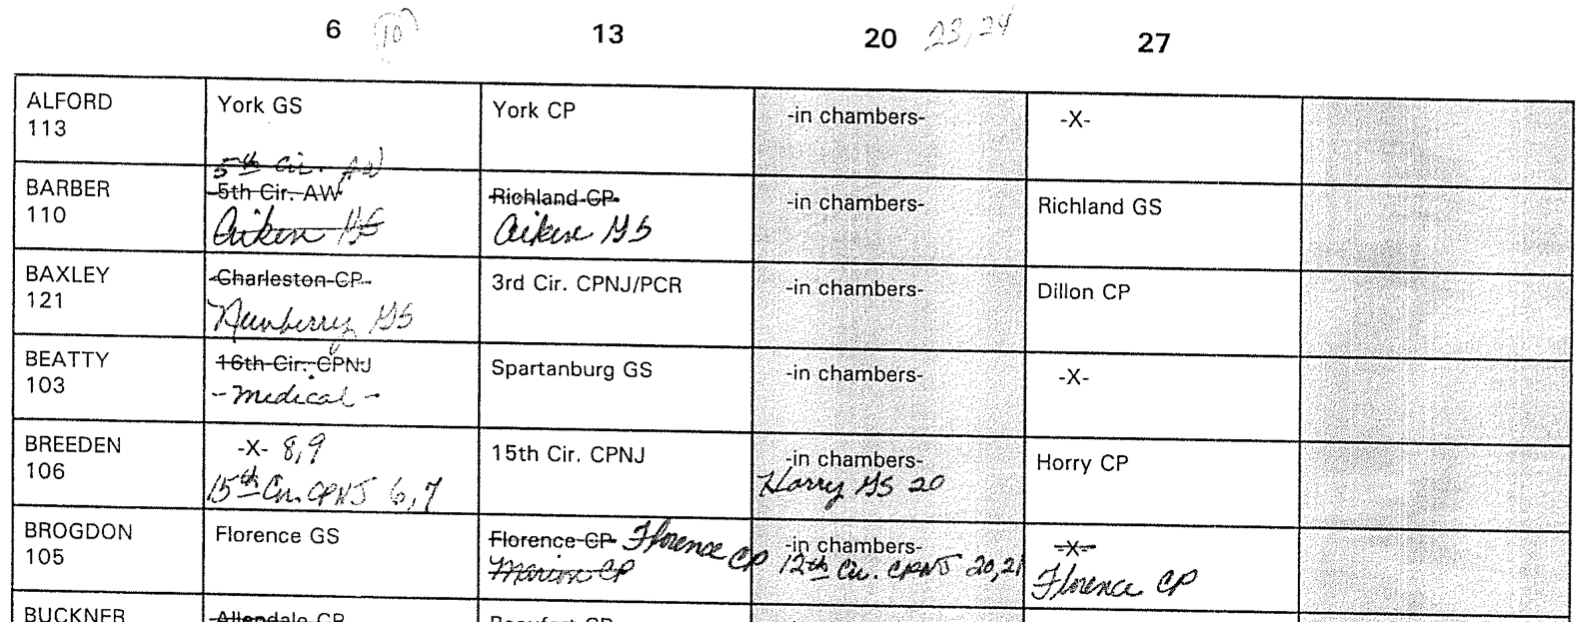
\includegraphics[scale=0.42]{Figures/Fig3A}
	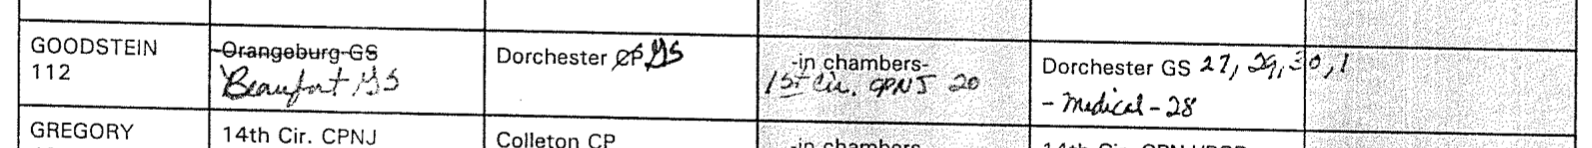
\includegraphics[scale=0.42]{Figures/Fig3B}
	\caption{Another snapshot of the November Calendar.}
	\label{Figure_Master_Calendar_3}
\end{figure}

\vspace{-3mm}
\paragraph{iii) Two Assignments (226 judge-week combinations).} 
\label{Category_iii}
This occurs in three ways. We discuss each case separately.
	\begin{itemize}
		\item[(a)] \emph{Neither assignment has a date (17 judge-week combinations).} For example, Judge Milling's assignment (on the master calendar) in the week of July 31st is Sumter GS and Malboro GS CC; see Figure \ref{Figure_Master_Calendar_4}. As will be discussed in Section \ref{Sec:Master_Calendar:Further_Analysis_of_Some_Assignments}, we only observe sentencing events in the counties stated on the master calendar for 15 of the 17 ($88.2\%$) judge-week combinations in this category. In other words, there are no inconsistencies between the master calendar and the sentencing dataset for 15 of these 17 judge-week combinations. The remaining 2 judge-week combinations are listed in Table \ref{Table_Mater_Calendar_Problematic_Cases_Detailed_Category_iii_a}.
		\item[(b)] \emph{One assignment has no dates while the other assignment has specific dates (163 judge-week combinations).} For example, Judge Breeden's assignment (on the master calendar) in the week on November 20th is Horry GS 20 and in chambers; see Figure \ref{Figure_Master_Calendar_0}. As will be discussed in Section \ref{Sec:Master_Calendar:Further_Analysis_of_Some_Assignments}, we only observe sentencing events in the counties stated on the master calendar and only on the days stated on the master calendar for 138 of the 163 ($84.7\%$) judge-week combinations in this category. In other words, there are no inconsistencies between the master calendar and the sentencing dataset for 138 of these 163 judge-week combinations. The remaining 25 judge-week combinations are listed in Table \ref{Table_Mater_Calendar_Problematic_Cases_Detailed_Category_iii_b}.
		\item[(c)] \emph{Both assignments have specific dates (54 judge-week combinations).} For example, Judge Goldstein's assignment (on the master calendar) in the week of July 27th is Dorchester GS 27,29,30,1, Medical 28; see Figure \ref{Figure_Master_Calendar_3}. As will be discussed in Section \ref{Sec:Master_Calendar:Further_Analysis_of_Some_Assignments}, we only observe sentencing events in the counties stated on the master calendar and only on the days stated on the master calendar for 45 of the 54 judge-week combinations of this category. In other words, there are no inconsistencies between the master calendar and the sentencing dataset for 45 of these 54 judge-week combinations. The remaining 9 judge-week combinations are listed in Table \ref{Table_Mater_Calendar_Problematic_Cases_Detailed_Category_iii_c}.
	\end{itemize}

\vspace{-3mm}
\paragraph{iv) Multiple Assignments (19 judge-week combinations).} 
\label{Category_iv}
This assignment category occurs in three ways.  
	\begin{itemize}
		\item[(a)] \emph{No assignment has a date (2 judge-week combinations).} In both judge-week combinations of this category, we only observe sentencing events in the counties stated on the master calendar. In other words, there are no inconsistencies between the master calendar and the sentencing dataset.
		\item[(b)] \emph{Some assignments have no dates while other assignments have specific dates (19 judge-week combinations).} We only observe sentencing events in the counties stated on the master calendar and only on the days stated on the master calendar for 18 of the 19 judge-week combinations of this category. In other words, there are no inconsistencies between the master calendar and the sentencing dataset for 18 of these 19 judge-week combinations. The remaining judge-week combination is depicted in Table \ref{Table_Mater_Calendar_Problematic_Cases_Detailed_Category_ivb}.
		\item[(c)] \emph{All assignments have specific dates (2 judge-week combinations).} We only observe sentencing events in the counties stated on the master calendar and only on the days stated on the master calendar for one of the two judge-week combinations of this category. In other words, there are no inconsistencies between the master calendar and the sentencing dataset for one of the two judge-week combinations. The other judge-week combination is depicted in Table \ref{Table_Mater_Calendar_Problematic_Cases_Detailed_Category_ivc}.
	\end{itemize}


\subsection{Further Analysis of the Master Calendar Assignments using the Sentencing Data Set}
\label{Sec:Master_Calendar:Further_Analysis_of_Some_Assignments}

This section studies the master calendar in further detail by comparing it to the sentencing dataset. In doing so, we take advantage of the mapping from judge numbers to judge names (to be discussed in Section \ref{Sec:Mapping_Judge_Numbers_To_Judge_Names}). Appendix \ref{Sec:Appendix:Master_Calendar_Interpretations} provides plausible assignments for the judges in the ambiguous cases based on the facts presented in this section.

\subsubsection{No Assignments Case}
\label{Sec:Master_Calendar:Further_Analysis_of_Some_Assignments:Category_i}
As illustrated in Figure \ref{Figure_Simultaneous_Assignment_Count_Histogram}, there are 110 judge-week combinations in Category i. We observe no sentencing events (in the sentencing dataset) for 101 out of these 110 ($91.8\%$) judge-week combinations. Recall that the judges in these combinations have no assignments on the master calendar. Therefore, there are no inconsistencies between the master calendar and the sentencing dataset for these 101 judge-week combinations. The remaining 9 judge-week combinations are listed in Table \ref{Table_Mater_Calendar_Problematic_Cases_Detailed_Category_i}. We observe at least one sentencing event (in the sentencing dataset) for these judge-week combinations. Each judge visits only one county (according to the sentencing dataset) in these 9 judge-week combinations.

\begin{table}[H]
	\centering
	\caption{Judge-week combinations in which the judge has sentencing events in a county to which he is not assigned - Category i. The first number in the parenthesis depicts the number of pleas and the second number depicts the number of trials.} 
	\vspace{-2mm}
	\hspace*{0mm}
	\setlength\tabcolsep{0pt} % default value: 6pt
	{\scriptsize
		\begin{tabular}{>{\quad}L{6mm}C{8mm}C{2mm}L{17mm}C{25mm}C{25mm}C{25mm}C{25mm}C{25mm}cccc}
			\toprule
			& & && \multicolumn{5}{c}{Sentencing Data Set} \\
			\cmidrule(ll){5-9} 
			& Judge && Week & Monday & Tuesday & Wednesday & Thursday & Friday \\
			\midrule
			%& \rowgroup{$\nquad$\textbf{No Sentences}} \\
			1  &  8  &&  January 29  & \textcolor{red}{Dorchester (1,0)}  &  &  &  &  \\
			2  &  8  &&  June 4 & \textcolor{red}{Orangeburg (5,0)}  &  & \textcolor{red}{Orangeburg (2,1)}  & \textcolor{red}{Orangeburg (4,0)}  &  \\
			3  &  8  &&  July 3  &  &  &  &  & \textcolor{red}{Dorchester (0,1)}  \\
			4  &  8  &&  July 24   & & \textcolor{red}{Orangeburg (1,0)}  & \textcolor{red}{Orangeburg (1,0)} &  & \textcolor{red}{Orangeburg (1,0)}  &  \\
			5  &  26  &&  April 23  & \textcolor{red}{Greenwood (1,0)}  &  &  &  &  \\
			6  &  26  &&  October 30  &  &  & \textcolor{red}{Greenwood (1,0)}  &  &  \\
			7  &  43  &&  March 12  &  &  & \textcolor{red}{Greenville (1,0)}  &  &  \\
			8  &  43  &&  April 16   &  & \textcolor{red}{Greenville (1,0)}  &  &  &  \\
			9  &  47  &&  October 23  & \textcolor{red}{Charleston (1,0)}  &  &  &  &  \\
			\bottomrule
		\end{tabular}
	}
	\label{Table_Mater_Calendar_Problematic_Cases_Detailed_Category_i}
\end{table}

\subsubsection{One Assignment Case} 
\label{Sec:Master_Calendar:Further_Analysis_of_Some_Assignments:Category_ii}
We start with Category ii (a), i.e., no dates are indicated. As illustrated in Figure \ref{Figure_Simultaneous_Assignment_Count_Histogram}, there are 2200 judge-week combinations in Category ii (a). Although in judge-week combinations of Category ii (a) (according to the master calendar) the judges have an assignment the entire week, they do not necessarily sentence every day of the week; see Figure \ref{Figure_Histogram_of_Number_of_Days_With_Sentences_Category_10} for a histogram of the number of days in the week with a sentencing event and Figure \ref{Figure_Histogram_of_Sentences_This_Week_Category_10} for a histogram of the number of sentencing events observed for the judge-week combinations of Category ii (a). For 1872 of the 2200 ($85.1\%$) judge-week combinations of Category ii (a), we only observe sentencing events in the county to which the judge is assigned, i.e., we do not observe sentencing events in a county other than the county to which the judge is assigned. In other words, there are no inconsistencies between the master calendar and the sentencing dataset for 1872 of these 2200 judge-week combinations. The remaining 328 judge-week combinations are listed in Table \ref{Table_Mater_Calendar_Problematic_Cases_Detailed_Category_i}. We observe at least one sentencing event (in the sentencing dataset) in a county to which the judge is not assigned in these judge-week combinations. %Figure \ref{Figure_Histogram_of_Number_of_Days_With_Sentences_Category_11Histogram_Maximum_Number_of_Counties_Visited_Category_10} provides a histogram of the highest number of counties visited on a day for the judge-week combinations in Category ii (a). 
%\begin{note}
%	As depicted in Figure \ref{Figure_Histogram_of_Number_of_Days_With_Sentences_Category_11Histogram_Maximum_Number_of_Counties_Visited_Category_10}, in about 200 of the judge-week combinations of Category ii (a), the judge visited more than one county on a day; e.g., see combination 7 of Table \ref{Table_Mater_Calendar_Problematic_Cases_Detailed_Category_iia}. We should decide what to do with these combiations. What type of information on these combinations do you think would help us?
%\end{note}

\begin{figure}[H]
	\centering
	\begin{minipage}{.45\textwidth}
		\centering
		\hspace*{-8mm}
		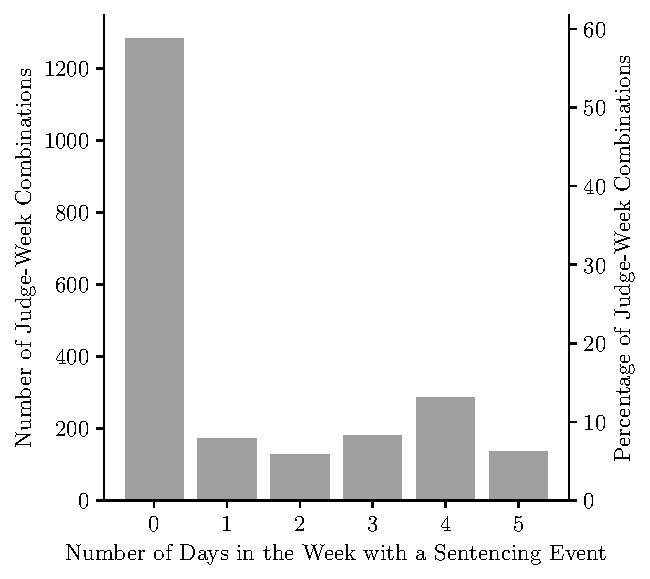
\includegraphics[scale=0.75]{Figures/Histogram_of_Number_of_Days_With_Sentences_Category_10}
		\hspace{4mm}
		\vspace{-6.0mm}
		\caption{A histogram of the number of days in the week with a sentencing event for judge-week combinations of Category ii (a).}
		\label{Figure_Histogram_of_Number_of_Days_With_Sentences_Category_10}
	\end{minipage}
	\hspace{5mm}
	\begin{minipage}{0.45\textwidth}
		\centering
		\hspace*{-3mm}
		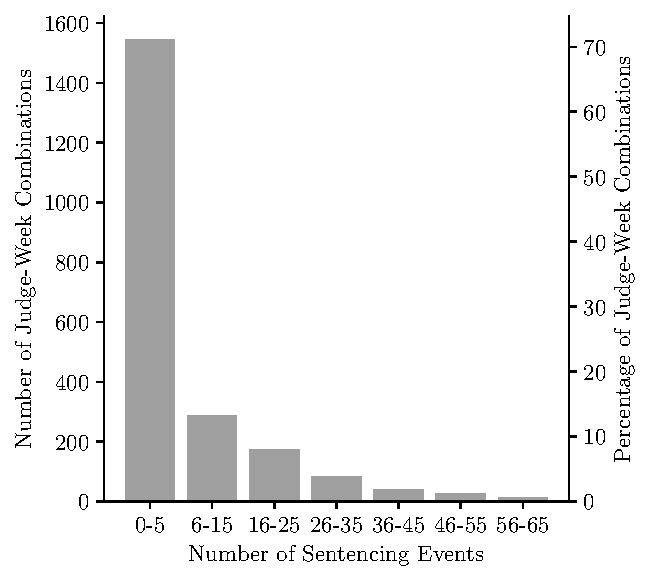
\includegraphics[scale=0.75]{Figures/Histogram_of_Sentences_This_Week_Category_10}
		\vspace{-6mm}
		\caption{A histogram of the number of sentencing events for judge-week combinations of Category ii (a).}
		\label{Figure_Histogram_of_Sentences_This_Week_Category_10}
	\end{minipage}
\end{figure}

%\begin{figure}[H]
%	\centering
%	\begin{minipage}{.45\textwidth}
%		\centering
%		\hspace*{-8mm}
%		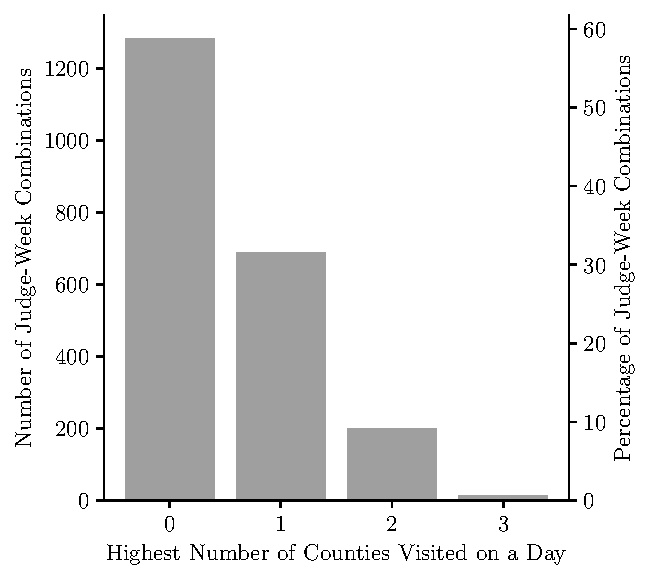
\includegraphics[scale=0.72]{Figures/Histogram_Maximum_Number_of_Counties_Visited_Category_10}
%		\hspace{4mm}
%		\vspace{-6.0mm}
%		\caption{A histogram of the highest number of counties visited on a day for judge-week combinations of Category ii (a).}
%		\label{Figure_Histogram_of_Number_of_Days_With_Sentences_Category_11Histogram_Maximum_Number_of_Counties_Visited_Category_10}
%	\end{minipage}
%	\hspace{5mm}
%	\begin{minipage}{0.45\textwidth}
%		\centering
%		\hspace*{-3mm}
%		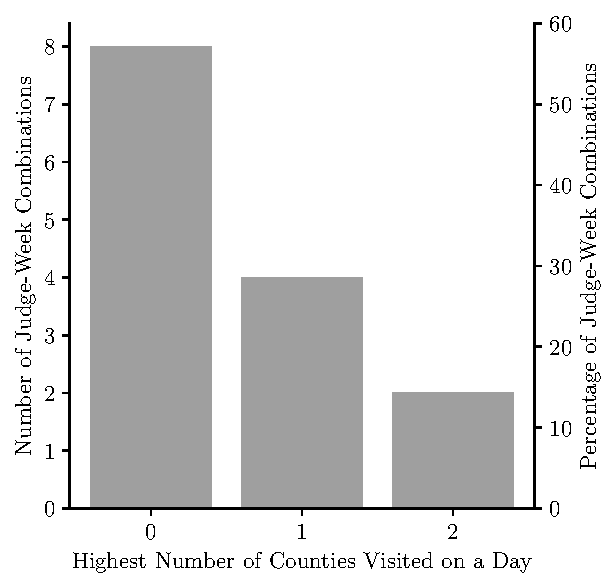
\includegraphics[scale=0.72]{Figures/Histogram_Maximum_Number_of_Counties_Visited_Category_11}
%		\vspace{-6mm}
%		\caption{A histogram of the highest number of counties visited on a day for judge-week combinations of Category ii (b).}
%		\label{Figure_Histogram_Maximum_Number_of_Counties_Visited_Category_11}
%	\end{minipage}
%\end{figure}

\begin{table}[H]
	\centering
	\caption{Judge-week combinations in which the judge has sentencing events in a county to which he is not assigned - Category ii (a). The counties written in green font are the counties to which the judge is assigned. The counties written in red font are the counties to which the judge is not assigned. The counties written in blue font are the counties to which the judge is not assigned, however, he is assigned to the circuit court containing these counties. So, the county assignment in the master calendar and this county belong to the same circuit court. The last column presents the percentage of the sentencing events (plea to trial, separately) that occurred in a county to which the judge is not assigned, i.e., it represents the fraction of sentencing events occurred in the counties written in red or blue fonts.} 
	\vspace{-2mm}
	\hspace*{-26.5mm}
	\setlength\tabcolsep{2pt} % default value: 6pt
	{\scriptsize
		\begin{tabular}{>{\quad}C{8mm}C{8mm}L{20mm}L{31mm}C{24mm}C{22mm}C{24mm}C{25mm}C{23mm}cc}
			\toprule
			& & & & \multicolumn{5}{c}{Sentencing Data Set} & \multicolumn{2}{c}{$\,\,\,$Percentage} \\
			\cmidrule(ll){5-9} \cmidrule(ll){10-11} 
			& Judge & Week & Master Calendar & Monday & Tuesday & Wednesday & Thursday & Friday & $\,\,\,$Plea & Trial \\
			\midrule
			1  &  2  &  January 8  & Chester GS  & \textcolor{green}{Chester (2,0)} & \textcolor{red}{York (1,0)} &  &  & \textcolor{green}{Chester (2,0)} & 20\% & 0\% 
			\\
			& & &  &  &  &  &  & & \\
			2  &  2  &  February 12  & Chester CP  &  &  &  & \textcolor{red}{Lancaster (1,0)} &  & 100\% & 0\% 
			\\
			& & &  &  &  &  &  & & \\
			3  &  2  &  June 4  & Chester GS  &  &  & \textcolor{green}{Chester (0,1)} & \textcolor{red}{Spartanburg (1,0)}, \textcolor{green}{Chester (2,0)} & \textcolor{green}{Chester (3,0)} & 14\% & 0\% 
			\\
			4  &  2  &  August 7  & York GS  &  & \textcolor{green}{York (2,0)} & \textcolor{green}{York (2,0)} & \textcolor{green}{York (4,0)} & \textcolor{red}{Kershaw (1,0)}, \textcolor{green}{York (7,0)} & 6\% & 0\% 
			\\
			5  &  2  &  August 21  & York GS  &  & \textcolor{green}{York (1,0)} &  &  & \textcolor{red}{Union (1,0)}, \textcolor{green}{York (2,0)} & 25\% & 0\% 
			\\
			6  &  2  &  September 11  & York GS  & \textcolor{green}{York (6,0)} & \textcolor{green}{York (2,0)} &  & \textcolor{green}{York (2,0)} & \textcolor{red}{Spartanburg (1,0)}, \textcolor{green}{York (5,0)} & 6\% & 0\% 
			\\
			7  &  2  &  October 9  & York GS  &  &  & \textcolor{red}{Fairfield (1,0)}, \textcolor{green}{York (1,0)} & \textcolor{green}{York (5,0)} & \textcolor{green}{York (4,0)} & 9\% & 0\% 
			\\
			8  &  2  &  October 23  & York GS  & \textcolor{green}{York (2,0)} & \textcolor{green}{York (3,0)} & \textcolor{green}{York (9,0)} & \textcolor{green}{York (1,0)} & \textcolor{red}{Kershaw (1,0)}, \textcolor{green}{York (6,0)} & 5\% & 0\% 
			\\
			9  &  3  &  January 8  & Bamberg GS  & \textcolor{green}{Bamberg (1,0)} & \textcolor{green}{Bamberg (3,0)} & \textcolor{green}{Bamberg (3,0)} &  & \textcolor{red}{Aiken (1,0)} & 12\% & 0\% 
			\\
			& & &  &  &  &  &  & & \\
			10  &  3  &  February 12  & Aiken GS  & \textcolor{green}{Aiken (9,0)} & \textcolor{green}{Aiken (3,0)} &  & \textcolor{red}{Edgefield (1,0)}, \textcolor{green}{Aiken (2,1)} & \textcolor{red}{Barnwell (1,0)}, \textcolor{green}{Aiken (2,0)} & 11\% & 0\% 
			\\
			\\
			. & . & . & . & . & . & . & . & . & . \\
			. & . & . & . & . & . & . & . & . & .  \\
			. & . & . & . & . & . & . & . & . & . \\
			& & &  &  &  &  &  & & \\
			318  &  50  &  October 16  & McCormick GS  &  & \textcolor{green}{McCormick (15,0)} & \textcolor{red}{Saluda (1,0)}, \textcolor{green}{McCormick (1,0)} &  &  & 6\% & 0\% 
			\\
			319  &  50  &  November 6  & 11th Cir. CPNJ  &  &  &  & \textcolor{blue}{Lexington (1,0)} &  & 100\% & 0\% 
			\\
			& & &  &  &  &  &  & & \\
			320  &  51  &  January 8  & Orangeburg GS  & \textcolor{red}{Calhoun (2,0)}, \textcolor{green}{Orangeburg (14,0)} & \textcolor{green}{Orangeburg (3,0)} & \textcolor{green}{Orangeburg (4,0)} & \textcolor{green}{Orangeburg (3,0)} & \textcolor{red}{Aiken (1,0)}, \textcolor{green}{Orangeburg (2,0)} & 10\% & 0\% 
			\\
			321  &  51  &  January 22  & Sumter GS  & \textcolor{red}{York (1,0)}, \textcolor{green}{Sumter (6,0)} & \textcolor{green}{Sumter (2,0)} & \textcolor{green}{Sumter (3,0)} & \textcolor{green}{Sumter (1,0)} & \textcolor{green}{Sumter (3,0)} & 6\% & 0\% 
			\\
			322  &  51  &  February 5  & Clarendon GS  & \textcolor{green}{Clarendon (3,0)} & \textcolor{green}{Clarendon (2,0)} & \textcolor{green}{Clarendon (1,0)} &  & \textcolor{red}{Sumter (1,0)}, \textcolor{green}{Clarendon (3,0)} & 10\% & 0\% 
			\\
			323  &  51  &  April 16  & Sumter GS  & \textcolor{red}{Clarendon (0,1)}, \textcolor{green}{Sumter (5,0)} & \textcolor{green}{Sumter (3,0)} & \textcolor{green}{Sumter (2,0)} & \textcolor{green}{Sumter (3,0)} & \textcolor{green}{Sumter (3,0)} & 0\% & 6\% 
			\\
			324  &  51  &  May 28  & 3rd Cir. CPNJ/PCR  &  &  &  & \textcolor{blue}{Sumter (1,0)} & \textcolor{blue}{Williamsburg (1,0)} & 100\% & 0\% 
			\\
			325  &  51  &  September 25  & Richland GS  & \textcolor{green}{Richland (7,0)} & \textcolor{red}{Lexington (1,0), Clarendon (1,0)} & \textcolor{green}{Richland (2,1)} & \textcolor{green}{Richland (3,0)} & \textcolor{green}{Richland (1,0)} & 12\% & 0\% 
			\\
			326  &  51  &  October 2  & in chambers  &  &  &  &  & \textcolor{red}{Richland (1,0)} & 100\% & 0\% 
			\\
			& & &  &  &  &  &  & & \\
			327  &  51  &  October 16  & Orangeburg GS  & \textcolor{green}{Orangeburg (14,0)} & \textcolor{green}{Orangeburg (2,0)} & \textcolor{green}{Orangeburg (5,0)} & \textcolor{red}{Charleston (1,0)}, \textcolor{green}{Orangeburg (3,0)} & \textcolor{green}{Orangeburg (1,0)} & 4\% & 0\% 
			\\
			328  &  51  &  December 18  & in chambers  & \textcolor{red}{Richland (1,0)} & \textcolor{red}{Richland (24,0)} &  &  &  & 100\% & 0\% 
			\\
			\bottomrule
		\end{tabular}
	}
	\label{Table_Mater_Calendar_Problematic_Cases_Detailed_Category_iia}
\end{table}

As illustrated in Figure \ref{Figure_Simultaneous_Assignment_Count_Histogram}, there are 14 judge-week combinations in Category ii (b), i.e., a single assignment with specific dates. Figure \ref{Figure_Histogram_of_Number_of_Days_With_Sentences_Category_11} provides a histogram of the number of days in the week with a sentencing event for the judge-week combinations of Category ii (b). Figure \ref{Figure_Histogram_of_Sentences_This_Week_Category_11} provides a histogram of the number of sentencing events observed for these 14 judge-week combinations. In 10 of the 14 judge-week combinations, we either observe no sentencing events (8 of them, as shown in Figure \ref{Figure_Histogram_of_Number_of_Days_With_Sentences_Category_11}) or sentencing events only in the same county as listed in the master calendar (2 of them). In other words, there are no inconsistencies between the master calendar and the sentencing dataset for 10 of these 14 ($71.4\%$) judge-week combinations. The remaining 4 judge-week combinations are listed in Table \ref{Table_Mater_Calendar_Problematic_Cases_Detailed_Category_i}. In these 4 judge-week combinations, exactly one of the following conditions holds:
\begin{enumerate}
	\vspace{-3mm}
	\item At least one sentencing event occurred in a county not stated on the master calendar (3 judge-week combinations); see the last three rows of Table \ref{Table_Mater_Calendar_Problematic_Cases_Detailed_Category_iib}.
	\vspace{-2mm}
	\item At least one sentencing event occurred in the county stated on the master calendar but on a date not stated on the master calendar (1 judge-week combination); see the first row of Table \ref{Table_Mater_Calendar_Problematic_Cases_Detailed_Category_iib}.
\end{enumerate}

\begin{table}[H]
	\centering
	\caption{Judge-week combinations in which the judge has sentencing events in a county to which he is not assigned - Category ii (b). The counties written in green font are the counties to which the judge is assigned. The counties written in red font are the counties to which the judge is not assigned. The last column presents the percentage of the sentencing events (plea or trial, separately) that occurred in a county to which the judge is not assigned, i.e., it represents the fraction of sentencing events occurred in the counties written in red font.} 
	\vspace{-2mm}
	\hspace*{-21mm}
	\setlength\tabcolsep{2pt} % default value: 6pt
	{\scriptsize
		\begin{tabular}{>{\quad}C{6mm}C{8mm}L{18mm}L{31mm}C{22mm}C{22mm}C{22mm}C{22mm}C{22mm}cc}
			\toprule
			& & & & \multicolumn{5}{c}{Sentencing Data Set} & \multicolumn{2}{c}{$\,\,\,$Percentage} \\
			\cmidrule(ll){5-9} \cmidrule(ll){10-11} 
			& Judge & Week & Master Calendar & Monday & Tuesday & Wednesday & Thursday & Friday & $\,\,\,$Plea & Trial \\
			\midrule
			1  &  7  &  March 19  & Horry GS CP CC 21,22,23  &  & \textcolor{red}{Horry (6,0)} &  & \textcolor{green}{Horry (5,0)} &  & 55\% & 0\% 
			\\
			2  &  28  &  September 25  & Bamberg GS 25,26,27,28,29  & \textcolor{red}{Lee (1,0)}, \textcolor{green}{Bamberg (10,0)} & \textcolor{green}{Bamberg (6,0)} &  &  &  & 6\% & 0\% 
			\\
			3  &  47  &  October 30  & Barnwell GS 1,2,3  &  &  & \textcolor{green}{Barnwell (1,0)} & \textcolor{red}{Allendale (1,0)}, \textcolor{green}{Barnwell (2,0)} &  & 25\% & 0\% 
			\\
			4  &  49  &  October 23  & 13th Cir. CPNJ 23,24,25,26  &  &  &  &  & \textcolor{red}{Clarendon (1,0)} & 100\% & 0\% 
			\\
			\bottomrule
		\end{tabular}
	}
	\label{Table_Mater_Calendar_Problematic_Cases_Detailed_Category_iib}
\end{table}

\begin{figure}[H]
	\centering
	\begin{minipage}{.45\textwidth}
		\centering
		\hspace*{-3mm}
		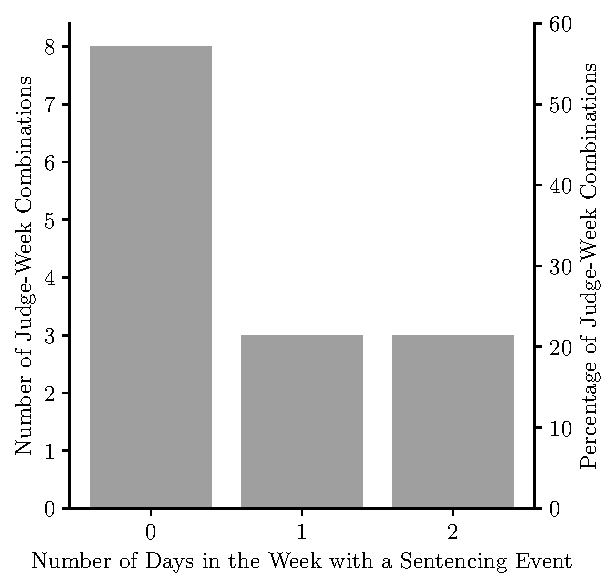
\includegraphics[scale=0.72]{Figures/Histogram_of_Number_of_Days_With_Sentences_Category_11}
		\hspace{4mm}
		\vspace{-6.0mm}
		\caption{A histogram of the number of days in the week with a sentencing event for judge-week combinations of Category ii (b).}
		\label{Figure_Histogram_of_Number_of_Days_With_Sentences_Category_11}
	\end{minipage}
	\hspace{5mm}
	\begin{minipage}{0.45\textwidth}
		\centering
		\hspace*{-3mm}
		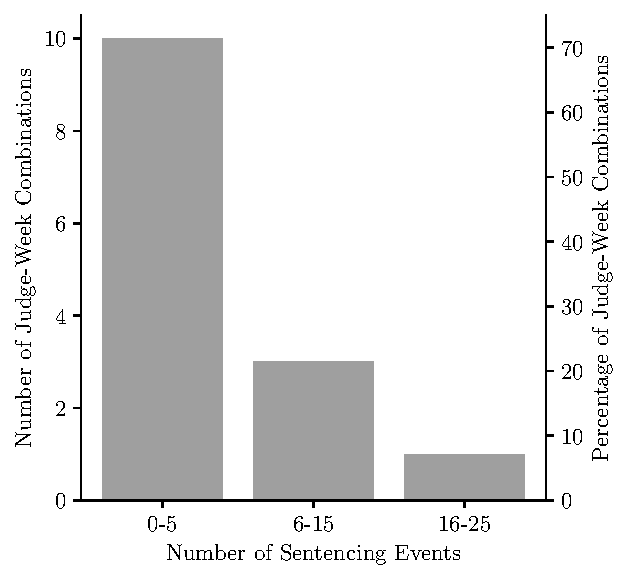
\includegraphics[scale=0.72]{Figures/Histogram_of_Sentences_This_Week_Category_11}
		\vspace{-6mm}
		\caption{A histogram of the number of sentencing events for judge-week combinations of Category ii (b).}
		\label{Figure_Histogram_of_Sentences_This_Week_Category_11}
	\end{minipage}
\end{figure}

\subsubsection{Two Assignments Case}
\label{Sec:Master_Calendar:Further_Analysis_of_Some_Assignments:Category_iii}
We start with Category iii (a), i.e., neither assignment has specific dates. As illustrated in Figure \ref{Figure_Simultaneous_Assignment_Count_Histogram}, there are 17 judge-week combinations in Category iii (a). For 15 of the 17 ($88.2\%$) judge-week combinations of Category iii (a), we only observe sentencing events in one of the two counties stated on the master calendar. In other words, there are no inconsistencies between the master calendar and the sentencing dataset for 15 of these 17 judge-week combinations. The remaining 2 judge-week combinations are listed in Table \ref{Table_Mater_Calendar_Problematic_Cases_Detailed_Category_iii_a}. The judge-week combinations of Category iii(a) that satisfy (at least) one of the following conditions are potentially problematic:
\begin{enumerate}
	\vspace{-3mm}
	\item At least one sentencing event occurred in a county not stated on the master calendar (Both rows of Table \ref{Table_Mater_Calendar_Problematic_Cases_Detailed_Category_iii_a}).
	\vspace{-2mm}
	\item The judge sentenced in more than one county on a day (First row of Table \ref{Table_Mater_Calendar_Problematic_Cases_Detailed_Category_iii_a}).
\end{enumerate}

\begin{table}[H]
	\centering
	\caption{Judge-week combinations in which the judge has sentencing events in a county to which he is not assigned - Category iii (a). The county written in green font is the county to which the judge is assigned. The counties written in red font are the counties to which the judge is not assigned. The county written in blue font is the county to which the judge is not assigned, however, he is assigned to the circuit court containing this county. So, the county assignment in the master calendar and this county belong to the same circuit court. The last column presents the percentage of the sentencing events (plea or trial, separately) that occurred in a county to which the judge is not assigned, i.e., it represents the fraction of sentencing events occurred in the counties written in red or blue fonts.} 
	\vspace{-2mm}
	\hspace*{-0mm}
	\setlength\tabcolsep{2pt} % default value: 6pt
	{\scriptsize
		\begin{tabular}{>{\quad}C{6mm}C{8mm}L{13mm}L{25mm}C{15mm}C{15mm}C{20mm}C{17mm}C{17mm}cc}
			\toprule
			& & & & \multicolumn{5}{c}{Sentencing Data Set} & \multicolumn{2}{c}{$\,\,\,$Percentage} \\
			\cmidrule(ll){5-9} \cmidrule(ll){10-11} 
			& Judge & Week & Master Calendar & Monday & Tuesday & Wednesday & Thursday & Friday & $\,\,\,$Plea & Trial \\
			\midrule
			1  &  3  &  April 30  & Aiken GS CC, 2nd Cir. CP/PCR  &  &  & \textcolor{blue}{Bamberg (1,0)}, \textcolor{green}{Aiken (5,0)} &  &  & 17\% & 0\% 
			\\
			2  &  10  &  January 8  & Florence GS, Lee GS  &  &  & \textcolor{red}{Marion (1,0)} & \textcolor{red}{Marion (1,0)} &  & 100\% & 0\% 
			\\
			\bottomrule
		\end{tabular}
	}
	\label{Table_Mater_Calendar_Problematic_Cases_Detailed_Category_iii_a}
\end{table}

For the judge-week combination in row 1 of Table \ref{Table_Mater_Calendar_Problematic_Cases_Detailed_Category_iii_a}, the judge (Judge 3) is assigned to Aiken and the 2nd circuit court (according to the master calendar). However, he has a sentencing event in Bamberg and Aiken on Wednesday. Bamberg belongs to the 2nd circuit court.

For the judge-week combination in row 2 of Table \ref{Table_Mater_Calendar_Problematic_Cases_Detailed_Category_iii_a}, the judge (Judge 10) is assigned to Florence and Lee (according to the master calendar). However, he has a sentencing event in Marion on Wednesday and another sentencing event in Marion on Thursday. 

As illustrated in Figure \ref{Figure_Simultaneous_Assignment_Count_Histogram}, there are 163 judge-week combinations in Category iii (b), i.e., one assignment has no dates whereas the other one has specific dates. For 138 of these 163 ($84.7\%$) judge-week combinations, we only observe sentencing events in one of the two counties stated on the master calendar and only on the days stated on the master calendar. In other words, there are no inconsistencies between the master calendar and the sentencing dataset for 138 of these 163 judge-week combinations. The remaining 25 judge-week combinations are listed in Table \ref{Table_Mater_Calendar_Problematic_Cases_Detailed_Category_iii_b}. 

\begin{table}[H]
	\centering
	\caption{Judge-week combinations in which the judge has sentencing events in a county to which he is not assigned - Category iii (b). The counties written in green font are the counties to which the judge is assigned. The counties written in red font are the counties to which the judge is not assigned. The counties written in blue font are the counties to which the judge is not assigned, however, he is assigned to the circuit court containing these counties. So, the county assignment in the master calendar and this county belong to the same circuit court. The last column presents the percentage of the sentencing events (plea or trial, separately) that occurred in a county to which the judge is not assigned, i.e., it represents the fraction of sentencing events occurred in the counties written in red or blue fonts.} 
	\vspace{-2mm}
	\hspace*{-21mm}
	\setlength\tabcolsep{2pt} % default value: 6pt
	{\scriptsize
		\begin{tabular}{>{\quad}C{6mm}C{8mm}L{17mm}L{30mm}C{22mm}C{22mm}C{24mm}C{23mm}C{22mm}cc}
			\toprule
			& & & & \multicolumn{5}{c}{Sentencing Data Set} & \multicolumn{2}{c}{$\,\,\,$Percentage} \\
			\cmidrule(ll){5-9} \cmidrule(ll){10-11} 
			& Judge & Week & Master Calendar & Monday & Tuesday & Wednesday & Thursday & Friday & $\,\,\,$Plea & Trial \\
			\midrule
			1  &  7  &  October 16  & Florence CP, Florence GS CC 20  &  &  &  & \textcolor{red}{Horry (1,0)} & \textcolor{green}{Florence (8,0)} & 11\% & 0\% 
			\\
			2  &  7  &  December 18  & in chambers, 12th Cir. CPNJ 18,19  & \textcolor{blue}{Marion (1,0)} &  &  &  &  & 100\% & 0\% 
			\\
			3  &  10  &  June 18  & Florence GS, Florence CP 21  & \textcolor{green}{Florence (5,0)} & \textcolor{green}{Florence (3,0)} & \textcolor{red}{Darlington (1,0)}, \textcolor{green}{Florence (17,0)} & \textcolor{green}{Florence (12,0)} & \textcolor{green}{Florence (5,0)} & 2\% & 0\% 
			\\
			4  &  11  &  June 4  & 8th Cir. CPNJ, Spartanburg GS CC 8  & \textcolor{blue}{Laurens (1,0)} &  &  &  &  & 100\% & 0\% 
			\\
			5  &  11  &  October 2  & in chambers, 7th Cir. CPNJ 2,3,5  &  &  &  & \textcolor{blue}{Spartanburg (3,0)} &  & 100\% & 0\% 
			\\
			6  &  13  &  March 5  & McCormick GS, Edgefield GS CC 8  & \textcolor{green}{McCormick (3,0)} &  &  & \textcolor{red}{Saluda (1,0)} &  & 25\% & 0\% 
			\\
			7  &  14  &  January 8  & Richland GS, Aiken GS CC 12  & \textcolor{green}{Richland (8,0)} & \textcolor{green}{Richland (3,0)} & \textcolor{green}{Richland (1,0)} &  & \textcolor{red}{Richland (0,1)} & 0\% & 8\% 
			\\
			8  &  14  &  August 28  & Williamsburg GS, Orangeburg GS CC 1  & \textcolor{green}{Williamsburg (3,0)} & \textcolor{green}{Williamsburg (4,0)} & \textcolor{red}{Sumter (1,0)}, \textcolor{green}{Williamsburg (2,0)} & \textcolor{green}{Williamsburg (6,0)} &  & 6\% & 0\% 
			\\
			9  &  14  &  December 11  & Lee GS, Aiken GS CC 15  & \textcolor{green}{Lee (1,0)} & \textcolor{green}{Lee (1,0)} &  &  & \textcolor{red}{Lee (0,2)} & 0\% & 50\% \\	
			\\
			10  &  18  &  March 12  & Spartanburg CP, Cherokee GS CC 15  &  &  & \textcolor{red}{Pickens (1,0)} & \textcolor{green}{Cherokee (1,0)} &  & 50\% & 0\% 
			\\
			11  &  26  &  February 26  & Greenwood GS, 8th Cir. CPNJ CC 26  & \textcolor{blue}{Greenwood (4,0)} & \textcolor{green}{Greenwood (10,0)} & \textcolor{green}{Greenwood (7,0)} & \textcolor{blue}{Abbeville (1,0), Laurens (1,0)} & \textcolor{blue}{Greenville (1,0)}, \textcolor{green}{Greenwood (5,0)} & 24\% & 0\% 
			\\
			12  &  27  &  November 13  & Greenwood GS, Medical 17  & \textcolor{red}{Anderson (1,0)} &  & \textcolor{green}{Greenwood (9,1)} & \textcolor{green}{Greenwood (5,0)} &  & 6\% & 0\% 
			\\
			13  &  29  &  March 19  & Darlington GS, Dillon GS CC 23  & \textcolor{green}{Darlington (1,0)} & \textcolor{green}{Darlington (8,0)} & \textcolor{red}{Chesterfield (1,0)}, \textcolor{green}{Darlington (9,0)} & \textcolor{green}{Darlington (3,0)} &  & 5\% & 0\% 
			\\
			14  &  29  &  July 31  & Richland GS, Lexington GS CC 3  & \textcolor{red}{Lexington (1,0)}, \textcolor{green}{Richland (13,0)} & \textcolor{red}{Marlboro (1,0), Kershaw (1,0)}, \textcolor{green}{Richland (10,0)} & \textcolor{green}{Richland (12,0)} & \textcolor{red}{Richland (4,0)} &  & 17\% & 0\% 
			\\
			15  &  30  &  June 4  & 16th Cir. CPNJ, Clarendon GS CC 8  &  & \textcolor{red}{Union (1,0)} &  &  & \textcolor{green}{Clarendon (1,0)} & 50\% & 0\% 
			\\
			16  &  31  &  October 2  & in chambers, Greenville GS 6  &  &  & \textcolor{red}{Anderson (1,0)} &  &  & 100\% & 0\% 
			\\
			17  &  33  &  April 9  & Charleston CP, Horry GS CC 9   & \textcolor{red}{Charleston (1,0)} &  &  &  &  & 100\% & 0\% 
			\\
			18  &  33  &  April 30  & Berkeley GS, Richland GS CC 2  & \textcolor{green}{Berkeley (6,0)} & \textcolor{green}{Berkeley (1,0)} & \textcolor{red}{Berkeley (2,0)} & \textcolor{green}{Berkeley (6,0)} &  & 13\% & 0\% 
			\\
			19  &  35  &  April 16  & Florence GS, 5th Cir. CPNJ CC 20  & \textcolor{green}{Florence (12,0)} & \textcolor{green}{Florence (8,0)} & \textcolor{green}{Florence (16,0)} & \textcolor{green}{Florence (5,0)} & \textcolor{red}{Florence (5,0)} & 11\% & 0\% 
			\\
			20  &  35  &  May 14  & Marion GS , 5th Cir. CPNJ CC 14  & \textcolor{red}{Marion (7,0)} &  & \textcolor{green}{Marion (1,0)} &  & \textcolor{green}{Marion (8,0)} & 44\% & 0\% 
			\\
			21  &  38  &  January 15  & Georgetown CP, Georgetown GS CC 19  &  &  &  & \textcolor{red}{Marion (0,2)} &  & 0\% & 100\% 
			\\
			22  &  40  &  August 28  & Anderson CP, Oconee GS CC 1  &  &  &  &  & \textcolor{red}{Anderson (1,0)} & 100\% & 0\% 
			\\
			23  &  40  &  November 6  & Anderson GS, 10th Cir. CPNJ CC 8  & \textcolor{red}{Greenville (1,0)}, \textcolor{green}{Anderson (3,0)} &  & \textcolor{red}{Anderson (8,0)} & \textcolor{green}{Anderson (10,0)} &  & 41\% & 0\% 
			\\
			24  &  44  &  May 7  & in chambers, 9th Cir. CPNJ 8  &  & \textcolor{red}{Colleton (0,1)} &  &  &  & 0\% & 100\% 
			\\
			25  &  48  &  December 4  & 15th Cir. CPNJ, Horry GS CP CC 5  & \textcolor{blue}{Horry (1,0)} &  &  &  &  & 100\% & 0\% 
			\\
			\bottomrule
		\end{tabular}
	}
	\label{Table_Mater_Calendar_Problematic_Cases_Detailed_Category_iii_b}
\end{table}

The judge-week combinations listed in Table \ref{Table_Mater_Calendar_Problematic_Cases_Detailed_Category_iii_b} satisfy (at least) one of the following conditions, which are problematic (some satisfy multiple conditions):\footnote{For example, judge-week combination 12 satisfies all four conditions. In judge-week combination 12, the assignment of Judge 29 in the week of July 31 is Richland GS and Lexington GS CC 3. Therefore, we would expect Judge 29 to be in Lexington on Thursday, and to be in Richland on Monday, Tuesday, Wednesday, and Friday. Since we observe sentencing events in Marlboro and Kershaw (alongside Richland) on Tuesday, judge-week combination 12 satisfies Conditions 1 and 4. Since we observe sentencing events in both Lexington and Richland on Monday, judge-week combination 12 satisfies Condition 3. Since we observe sentencing events in Richland on Thursday, judge-week combination 12 satisfies Condition 2, as well.}
	\begin{enumerate}
		\vspace{-3mm}
		\item At least one sentencing event occurred in a county not stated on the master calendar, e.g., judge-week combination 2 of Table \ref{Table_Mater_Calendar_Problematic_Cases_Detailed_Category_iii_b} (17 such judge-week combinations are listed in Table \ref{Table_Mater_Calendar_Problematic_Cases_Detailed_Category_iii_b}).
		\vspace{-9mm}
		\item At least one sentencing event occurred in the county stated on the master calendar with specific dates, but on a date other than the dates specified, e.g., judge-week combination 23 of Table \ref{Table_Mater_Calendar_Problematic_Cases_Detailed_Category_iii_b} (4 such judge-week combinations are listed in Table \ref{Table_Mater_Calendar_Problematic_Cases_Detailed_Category_iii_b}.).
		\vspace{-2mm}
		\item At least one sentencing event occurred in the county stated on the master calendar without specific dates. However, this sentencing event occurred on a date specified for the other county, e.g., judge-week combination 8 of Table \ref{Table_Mater_Calendar_Problematic_Cases_Detailed_Category_iii_b} (8 such judge-week combinations are listed in Table \ref{Table_Mater_Calendar_Problematic_Cases_Detailed_Category_iii_b}.).
		\vspace{-2mm}
		\item The judge sentenced in more than one county on a day, e.g., judge-week combination 3 of Table \ref{Table_Mater_Calendar_Problematic_Cases_Detailed_Category_iii_b} (5 such judge-week combinations are listed in Table \ref{Table_Mater_Calendar_Problematic_Cases_Detailed_Category_iii_b}.).
\end{enumerate}
\vspace{-3mm}

As illustrated in Figure \ref{Figure_Simultaneous_Assignment_Count_Histogram}, there are 54 judge-week combinations in Category iii (c), i.e., both assignments have specific dates. For 45 of these 54 ($83.3\%$) judge-week combinations, we only observe sentencing events in one of the two counties stated on the master calendar and only on the days stated on the master calendar. In other words, there are no inconsistencies between the master calendar and the sentencing dataset for 45 of these 54 judge-week combinations. The remaining 9 judge-week combinations are listed in Table \ref{Table_Mater_Calendar_Problematic_Cases_Detailed_Category_iii_c}.

\begin{table}[H]
	\centering
	\caption{Judge-week combinations in which the judge has sentencing events in a county to which he is not assigned - Category iii (c). The counties written in green font are the counties to which the judge is assigned. The counties written in red font are the counties to which the judge is not assigned. The counties written in blue font are the counties to which the judge is not assigned, however, he is assigned to the circuit court containing these counties. So, the county assignment in the master calendar and this county belong to the same circuit court. The last column presents the percentage of the sentencing events (plea or trial, separately) that occurred in a county to which the judge is not assigned, i.e., it represents the fraction of sentencing events occurred in the counties written in red or blue fonts.} 
	\vspace{-2mm}
	\hspace*{-20mm}
	\setlength\tabcolsep{2pt} % default value: 6pt
	{\scriptsize
		\begin{tabular}{>{\quad}C{6mm}C{8mm}L{17mm}L{29mm}C{22mm}C{22mm}C{22mm}C{23mm}C{22mm}cc}
			\toprule
			& & & & \multicolumn{5}{c}{Sentencing Data Set} & \multicolumn{2}{c}{$\,\,\,$Percentage} \\
			\cmidrule(ll){5-9} \cmidrule(ll){10-11} 
			& Judge & Week & Master Calendar & Monday & Tuesday & Wednesday & Thursday & Friday & $\,\,\,$Plea & Trial \\
			\midrule
			&&\rowgroup{$\nquad\nquad\nquad\nquad$\textbf{Subcategory (c)}} \\
			1  &  6  &  October 16  & 15th Cir. AW 16,19,20, Aiken 17,18  &  & \textcolor{green}{Aiken (11,0)} & \textcolor{green}{Aiken (11,0)} & \textcolor{blue}{Horry (6,0), Williamsburg (1,0)} & \textcolor{blue}{Horry (1,0)} & 27\% & 0\% 
			\\
			2  &  10  &  July 10  & Darlington GS 11,12,13,14, XX 10  &  & \textcolor{green}{Darlington (2,0)} & \textcolor{green}{Darlington (5,0)} & \textcolor{red}{Chesterfield (1,0)}, \textcolor{green}{Darlington (9,0)} &  & 6\% & 0\% 
			\\
			3  &  17  &  November 27  & XX 1, Aiken GS 27,28,29,30  & \textcolor{green}{Aiken (3,0)} &  & \textcolor{green}{Aiken (1,1)} & \textcolor{red}{Spartanburg (1,0)}, \textcolor{green}{Aiken (7,0)} &  & 8\% & 0\% 
			\\
			4  &  18  &  April 16  & 13th Cir. CPNJ 16, Lexington GS 17,18,19,20  &  &  & \textcolor{green}{Lexington (12,0)} & \textcolor{red}{Richland (1,0)}, \textcolor{green}{Lexington (11,0)} &  & 4\% & 0\% 
			\\
			5  &  27  &  May 28  & 10th Cir. CPNJ/PCR 28,29,30, Lexington GS 31,1  &  &  & \textcolor{blue}{Anderson (1,0)} & \textcolor{green}{Lexington (15,0)} & \textcolor{green}{Lexington (1,0)} & 6\% & 0\% 
			\\
			6  &  35  &  January 8  & 12th Cir. CPNJ 8,9,11,12, X 10  & \textcolor{red}{Richland (1,0)} &  &  &  &  & 100\% & 0\% 
			\\
			7  &  40  &  October 30  & Anderson CP 1,2,3, Barnwell GS 30,31  & \textcolor{green}{Barnwell (3,0)} & \textcolor{red}{Newberry (1,0), Aiken (1,0)}, \textcolor{green}{Barnwell (13,0)} &  &  &  & 11\% & 0\% 
			\\
			8  &  44  &  May 14  & Colleton GS 14,15,16, X 17,18  & \textcolor{green}{Colleton (4,0)} & \textcolor{green}{Colleton (2,0)} & \textcolor{green}{Colleton (3,0)} &  & \textcolor{red}{Beaufort (1,0)} & 10\% & 0\% 
			\\
			9  &  50  &  July 17  & Lexington GS 17,18,19,20, X 21  &  &  & \textcolor{green}{Lexington (14,0)} & \textcolor{green}{Lexington (10,0)} & \textcolor{red}{Lexington (2,0)} & 8\% & 0\% 
			\\
			\bottomrule
		\end{tabular}
	}
	\label{Table_Mater_Calendar_Problematic_Cases_Detailed_Category_iii_c}
\end{table}

The judge-week combinations listed in Table \ref{Table_Mater_Calendar_Problematic_Cases_Detailed_Category_iii_c} satisfy (at least) one of the following conditions, which are problematic (some satisfy multiple conditions):\footnote{For example, judge-week combination 1 satisfies Conditions 1 and 3. In judge-week combination 1, the assignment of Judge 6 in the week of October 16 is 15th circuit court AW 16,19,20 and Aiken 17,18. Therefore, we would expect Judge 6 to be in the 15th circuit court on Monday, Thursday, and Friday, and to be in Aiken on Tuesday and Wednesday. Since we observe sentencing events in Horry and Williamsburg on Thursday, judge-week combination 1 satisfies both Conditions 1 and 3.}
\begin{enumerate}
	\vspace{-3mm}
	\item At least one sentencing event occurred in a county not stated on the master calendar, e.g., judge-week combination 1 of Table \ref{Table_Mater_Calendar_Problematic_Cases_Detailed_Category_iii_c} (8 such judge-week combinations are listed in Table \ref{Table_Mater_Calendar_Problematic_Cases_Detailed_Category_iii_c}).
	\vspace{-2mm}
	\item At least one sentencing event occurred in the county stated on the master calendar with specific dates, but on a date other than the dates specified (only one such judge-week combination is listed in Table \ref{Table_Mater_Calendar_Problematic_Cases_Detailed_Category_iii_c}; see the last row of the table).
	\vspace{-2mm}
	\item The judge sentenced in more than one county on a day, e.g., judge-week combination 1 of Table \ref{Table_Mater_Calendar_Problematic_Cases_Detailed_Category_iii_c} (5 such judge-week combinations are listed in Table \ref{Table_Mater_Calendar_Problematic_Cases_Detailed_Category_iii_c}).
\end{enumerate}
\vspace{-3mm}

\subsubsection{Multiple Assignments Case}
\label{Sec:Master_Calendar:Further_Analysis_of_Some_Assignments:Category_iv}

As illustrated in Figure \ref{Figure_Simultaneous_Assignment_Count_Histogram}, there are 2 judge-week combinations in Category iv (a), i.e., no assignments have dates. For both of these judge-week combinations, we only observe sentencing events in the counties stated on the master calendar and only on the days stated on the master calendar. In other words, there are no inconsistencies between the master calendar and the sentencing dataset. However, in one of the judge-week combinations, we observe sentencing events in two counties on a day. This judge-week combination is depicted in Table \ref{Table_Mater_Calendar_Problematic_Cases_Detailed_Category_iva}. There were judge-week combinations in Categories ii and iii, in which the judge had sentencing events in multiple counties on a day. However, in those judge-week combinations, the judge was not assigned to at least one of the counties on that date. Those judge-week combinations were covered in Tables \ref{Table_Mater_Calendar_Problematic_Cases_Detailed_Category_iia}-\ref{Table_Mater_Calendar_Problematic_Cases_Detailed_Category_iii_c}.

\begin{table}[H]
	\centering
	\caption{Judge-week combinations in which the judge has multiple sentencing events in two different counties on a day - Category iv (a).} 
	\vspace{-2mm}
	\hspace*{-10mm}
	\setlength\tabcolsep{2pt} % default value: 6pt
	{\scriptsize
		\begin{tabular}{>{\quad}C{6mm}C{8mm}L{20mm}L{27mm}C{17mm}C{17mm}C{17mm}C{17mm}C{20mm}cc}
			\toprule
			& & & & \multicolumn{5}{c}{Sentencing Data Set} & \multicolumn{2}{c}{$\,\,\,$Percentage} \\
			\cmidrule(ll){5-9} \cmidrule(ll){10-11} 
			& Judge & Week & Master Calendar & Monday & Tuesday & Wednesday & Thursday & Friday & $\,\,\,$Plea & Trial \\
			\midrule
			1 & 3 & April 30 & Aiken, Bamberg, Barnwell & & Bam. (11), Barn. (1) & Bam. (2), Barn. (5)& & Aiken (21) & 0\% & 0\% \\
			\bottomrule
		\end{tabular}
	}
	\label{Table_Mater_Calendar_Problematic_Cases_Detailed_Category_iva}
\end{table}

As illustrated in Figure \ref{Figure_Simultaneous_Assignment_Count_Histogram}, there are 19 judge-week combinations in Category iv (b), i.e., some assignments have specific dates, while others do not. For 18 of these 19 judge-week combinations, we only observe sentencing events in the counties stated on the master calendar and only on the days stated on the master calendar. In other words, there are no inconsistencies between the master calendar and the sentencing dataset. The remaining 1 judge-week combination is depicted in Table \ref{Table_Mater_Calendar_Problematic_Cases_Detailed_Category_ivb}, where a sentencing event occurred in a county not stated on the master calendar.

\begin{table}[H]
	\centering
	\caption{Judge-week combinations in which the judge has sentencing events in a county to which he is not assigned - Category iv (b). The county written in red font is the county to which the judge is not assigned. The last column presents the percentage of the sentencing events (plea or trial, separately) that occurred in a county to which the judge is not assigned, i.e., it represents the fraction of sentencing events written in red font.} 
	\vspace{-2mm}
	\hspace*{-10mm}
	\setlength\tabcolsep{2pt} % default value: 6pt
	{\scriptsize
		\begin{tabular}{>{\quad}C{6mm}C{8mm}L{20mm}L{27mm}C{17mm}C{17mm}C{17mm}C{17mm}C{20mm}cc}
			\toprule
			& & & & \multicolumn{5}{c}{Sentencing Data Set} & \multicolumn{2}{c}{$\,\,\,$Percentage} \\
			\cmidrule(ll){5-9} \cmidrule(ll){10-11} 
			& Judge & Week & Master Calendar & Monday & Tuesday & Wednesday & Thursday & Friday & $\,\,\,$Plea & Trial \\
			\midrule
			1  &  41  &  May 7  & in chambers, Greenville GS(SGJ) 7, 13th Cir. CPNJ 8  & \textcolor{red}{Spartanburg (1,0)} &  &  &  &  & 100\% & 0\% \\
			\bottomrule
		\end{tabular}
	}
	\label{Table_Mater_Calendar_Problematic_Cases_Detailed_Category_ivb}
\end{table}

As illustrated in Figure \ref{Figure_Simultaneous_Assignment_Count_Histogram}, there are 3 judge-week combinations in Category iv (c), i.e., all assignments have specific dates. For two of these three judge-week combinations, we only observe sentencing events in the counties stated on the master calendar and only on the days stated on the master calendar. In other words, there are no inconsistencies between the master calendar and the sentencing dataset in two of these three judge-week combinations. The other judge-week combination is depicted in Table \ref{Table_Mater_Calendar_Problematic_Cases_Detailed_Category_ivc}, where a sentencing event occurred in a county not stated on the master calendar.

\begin{table}[H]
	\centering
	\caption{Judge-week combinations in which the judge has sentencing events in a county to which he is not assigned - Category iv (c). The county written in blue font is the county to which the judge is not assigned, however, he is assigned to the circuit court containing these counties. So, the county assignment in the master calendar and this county belong to the same circuit court. The last column presents the percentage of the sentencing events (plea or trial, separately) that occurred in a county to which the judge is not assigned, i.e., it represents the fraction of sentencing events occurred in the county written in blue font.} 
	\vspace{-2mm}
	\hspace*{-18mm}
	\setlength\tabcolsep{2pt} % default value: 6pt
	{\scriptsize
		\begin{tabular}{>{\quad}C{6mm}C{8mm}L{20mm}L{36mm}C{20mm}C{20mm}C{20mm}C{20mm}C{20mm}cc}
			\toprule
			& & & & \multicolumn{5}{c}{Sentencing Data Set} & \multicolumn{2}{c}{$\,\,\,$Percentage} \\
			\cmidrule(ll){5-9} \cmidrule(ll){10-11} 
			& Judge & Week & Master Calendar & Monday & Tuesday & Wednesday & Thursday & Friday & $\,\,\,$Plea & Trial \\
			\midrule
			1  &  31  &  February 26  & Anderson CP 26,27,28,1, Cherokee GS 2, 10th Cir. CPNJ/GS 2  &  &  &  &  & \textcolor{blue}{Oconee (6,0)} & 100\% & 0\% 
			\\
			\bottomrule
		\end{tabular}
	}
	\label{Table_Mater_Calendar_Problematic_Cases_Detailed_Category_ivc}
\end{table}

\section{Mapping Judge Numbers to Judge Names}
\label{Sec:Mapping_Judge_Numbers_To_Judge_Names}

Recall that the master calendar lists the judge names and the counties they are assigned to each week. Also, recall that the judge names are not recorded in the sentencing dataset. Instead, the judges are numbered. This section maps the judge numbers in the sentencing dataset to the judge names in the master calendar. To do so, for each judge, we create a sequence of weekly county assignments. We do so using both the sentencing dataset (using the sentencing events and their dates) and the master calendar, resulting in two sequences of weekly county assignments for each judge. We compare these two sequences to find the mapping from the judge numbers to the judge names under the following assumptions. The justification for this assumption is discussed below after presenting the matching algorithm and the resulting mapping.
%
\begin{assumption}
	We restrict attention to the county name in the assignments listed on the master calendar when constructing the mapping from the judge numbers in the sentencing dataset to the judge names in the master calendar.
	\label{Assumption_Mapping_Only_County_Assignment_Matter} 
\end{assumption}
%
For each judge, in order to measure how close the aforementioned two sequences of weekly county assignments are, we start off by comparing these sequences week by week, i.e., componentwise. To do so, fix a judge and a week, and consider the list of counties for that week in each sequence. In particular, we consider the following two notions of match:
%
\vspace{-3mm}
\paragraph{Perfect Componentwise Match.} If the set of counties visited by the judge number (obtained from the sentencing dataset) is a subset of the set of counties assigned to the judge name (obtained from the master calendar), the two sets constitute a perfect componentwise match. Otherwise, they do not constitute a perfect componentwise match. They constitute a mismatch (under the perfect componentwise matching criterion). For example, let us consider Judge 25 and Judge Hayes in the week of July 10th. In the week of July 10th, Judge 25 had sentencing events in \{York\} and Judge Hayes was assigned to \{York\}. These two sets (of counties) constitute a perfect componentwise match. 
%
\vspace{-3mm}
\paragraph{Overlapping Componentwise Match.} If the intersection of the two sets is non-empty, they constitute an overlapping componentwise match. Otherwise, they constitute a mismatch (under the overlapping componentwise matching criterion). For example, let us consider Judge 25 and Judge Hayes in the week of July 17th. In the week of July 17th, Judge 25 had sentencing events in \{Union,Spartanburg\} and Judge Hayes was assigned to \{Union\}. These two sets (of counties) constitute an overlapping componentwise match. Note that this would be a mismatch under the perfect componentwise matching criterion.

Then, we use the following algorithm to map the judge numbers (in the sentencing dataset) to the judge names (in the master calendar). The algorithm seeks to map each judge number to the judge name for which the number of matching weeks is maximal.
%
\vspace{-3mm}
\paragraph{Algorithm.} Choose the matching criterion.
%
\vspace{-5mm}
\paragraph{Step 0.} Fix a judge number. Find the set of judge names that have zero weeks of mismatch with the judge number under consideration. Then, map each judge number to the judge name with which it has zero weeks of mismatch. Repeat this process for all judge numbers. Next, drop the mapped judge numbers and judge names from the consideration list and proceed to the next step. 
%
\vspace{-5mm}
\paragraph{Step 1.} Fix an unmapped judge number. Find the set of unmapped judge names that have $1$ week of mismatch with the judge number under consideration. Then, map each unmapped judge number to the judge name with which it has $1$ week of mismatch. Repeat this process for all unmapped judge numbers. Next, drop the mapped judge numbers and judge names from the consideration list. If any of the (non-fictitious) judge numbers are not yet mapped, proceed to the next step.
%
\vspace{-5mm}
\paragraph{Step $n>1$.} Fix an unmapped judge number. Find the set of unmapped judge names that have $n$ weeks of mismatch with the judge number under consideration. Then, map each unmapped judge number to the judge name with which it has $n$ weeks of mismatch. Repeat this process for all unmapped judge numbers. Next, drop the mapped judge numbers and judge names from the consideration list. If any judge numbers are not yet mapped, proceed to the next step. Continue this process until all judge numbers are mapped to a judge name.

We obtain the same alphabetical mapping under both matching criterion; see Table \ref{Table_Mapping_Judge_Numbers_To_Judge_Names} (in Appendix \ref{Sec:Appendix:Supplementary_Tables}). Figure \ref{Figure_Mapping_Mismatches} (in Appendix \ref{Sec:Appendix:Supplementary_Figures}) depicts the number of weeks of mismatch between the judge numbers and the judge names. In particular, it shows that for all judge numbers, the mapped judge name has considerably fewer weeks of mismatch than any other judge name. In particular, there were no ties.

Next, we assess the performance of the (derived) mapping (from the judge numbers to the judge names). Under this mapping, we observe that only in $4.1\%$ of the sentencing events with a date, the judge was sentencing in a county to which he was not assigned. These $4.1\%$ problematic sentencing events belong to one of two categories: About $0.9\%$ belong to judge-week combinations in which the judge did not have any county assignments on the master calendar. The remaining $3.2\%$ belong to judge-week combinations in which the judge had county assignments on the master calendar. However, he was not assigned to the county in which the sentencing event occurred. Figure \ref{Figure_Mapping_Problematic_Sentencing_Events_Judge_Distribution} (in Appendix \ref{Sec:Appendix:Supplementary_Figures}) depicts the number of problematic sentencing events for each judge number. Figure \ref{Figure_Mapping_Problematic_Sentencing_Events_Week_Distribution} (in Appendix \ref{Sec:Appendix:Supplementary_Figures}) depicts the number of problematic sentencing events for each week. Figures \ref{Figure_Mapping_Problematic_Sentencing_Events_Judge_Distribution}-\ref{Figure_Mapping_Problematic_Sentencing_Events_Week_Distribution} show that the problematic sentencing events are not concentrated in just some judges or some weeks. These problematic sentencing events are discussed in detail in Section \ref{Sec:Master_Calendar:Further_Analysis_of_Some_Assignments}.

Assumption \ref{Assumption_Mapping_Only_County_Assignment_Matter} ignores the "circuit" assignments on the master calendar. Each circuit contains multiple counties. Instead, our matching algorithm works with the most granular geographic unit of interest, the county. As mentioned above, 3.2\% of the sentencing events with dates are at odds with the master calendar under the alphabetical mapping depicted in Table \ref{Table_Mapping_Judge_Numbers_To_Judge_Names}. Including "circuit" assignments and matching them on the basis of circuit courts as opposed to counties addresses only 12\% of the problematic sentencing events (corresponding to $0.4\%$ of the total number of sentencing events). As such, we stick with the choice of county for the matching purposes because it is more granular, and likely more accurate. Other assignments we ignore should be harmless because judges would not be involved in sentencing events or trials in those cases; see Figure  \ref{Figure_Assignment_Histogram}.

In addition, we focus only on the county names as opposed to the county name and the type of the assignment, which may also be listed; see Figure \ref{Figure_Assignment_Type_Histogram}. For example, Georgetown GS and Georgetown CP are both taken as Georgetown. There are several reasons for this: First, the type of the assignment is not always available. More importantly, all sentencing events should happen only in the general sessions (GS); and the common plea (CP) designation could be an error if a sentencing event appears in the sentencing dataset for the corresponding judge-week-county triple. Moreover, if no sentencing event occurs, then it is harmless to omit the CP designation. Consequently, focusing on the county name only makes the match easier.

Table \ref{Table_Schedule_Of_Unmapped_Judge_Names} (in Appendix \ref{Sec:Appendix:Supplementary_Figures}) depicts the list of counties visited by the fictitious judge (Juge 1) alongside the list of counties to which the unmapped judge names were assigned. Table \ref{Table_Schedule_Of_Unmapped_Judge_Names} shows that judge 1 is not a combination of the unmapped judge names.

\section{An Outline of the Model and its Calibration}
In order to facilitate the discussion in this section, recall the following notation used in the 3-agent model described in \citet[Chapter 3]{Can_Disseration}: Given a defendant, a judge, and a prosecutor, we let
\begin{itemize}
	\item[] $\theta$: the probability of conviction at trial (independent of the judge)
	\item[] $\tau$: the (expected) sentence length upon conviction at trial (independent of the judge)
	\item[] $c_d$: trial cost of the defendant
	\item[] $c_p$: trial cost of the prosecutor
	\item[] $u$: upper limit on a plea offer to which the judge would agree
	\item[] $l$: lower limit on a plea offer to which the judge would agree
	\item[] $v$: the defendant's visibility into judge schedules
	\item[] $r$: the maximum number of weeks the defendant can delay
	his/her sentence
	\item[] $d$: cost of waiting
\end{itemize}
The analysis below relies on the following results on the 3-agent model: Assuming $u\geq \theta\tau - c_p$ for simplicity, the prosecutor makes the plea offer $s=\max(\min(\theta \tau+c_d,u),l)$ and the defendant accepts it if $\theta \tau +c_d \geq l$. Otherwise, i.e., $\theta \tau + c_d < l$, then the case goes to trial. Moreover, the defendant's cost is $\min(\theta \tau+c_d,u)$ regardless of whether the case goes to trial or not.

Also, currently, South Carolina posts judge schedules well into the future on its website.\footnote{\url{https://www.sccourts.org/calendar/dspCCJudgeAsgMenu.cfm}.} As such, we will set $v=\infty$ for simplicity. Thus, a defendant can choose among the next $r$ weeks for his/her sentencing.

\subsection{Estimation of the Probability of Conviction at Trial $\theta$ and the Expected Sentence length $\tau$ upon Conviction at Trial as a Function of the Defendant Covariates}
\label{Sec:Estimation:Probability_Of_Conviction_And_Sentence_Length}
A defendant is characterized by $(\theta,\tau,c_d)$. Focusing on the cases which went to trial, we can estimate $\theta$ and $\tau$ using the logistic-negative Binomial regression model of \citet{Hester_Hartman_2017}; see Equations (1)-(2) of \citet{Hester_Hartman_2017}.
\begin{remark}
	Is it plausible that $\tau$ depends on the judge, i.e., $\tau(h)$? It appears that Can's analysis of the 3-agent game carries over to that case. However, this may require more data than we have. Nonetheless, if we group judges according to their harshness levels, we can probably handle this with the data we have.
\end{remark}

\subsection{Judge Harshness Analysis}
\label{Sec:Judge_Harshness_Analysis}

\vspace{-3mm}
\paragraph{A Simple Approach To Rank Judges with Respect to Their Harshness.} Focusing only on the plea bargains, we consider the logistic-negative Binomial model of \citet{Hester_Hartman_2017}. But, we also add a judge fixed effect dummy as a covariate. Then, we can rank judges according to the values of the judge fixed effects and group the judges accordingly if needed.
%
\vspace{-3mm}
\paragraph{Imputing $l$ and $u$ for Each Judge as a Function of $\theta\tau$.} Recall that a key quantity for us is $\theta\tau$. Fix a judge, say judge $j$, and focus only on the plea-bargains he ruled on. For each such case, we can calculate $\hat{\theta}\hat{\tau}$ using the estimates from the logistic-negative Binomial regression analysis of Section \ref{Sec:Estimation:Probability_Of_Conviction_And_Sentence_Length}. Suppose judge $j$ handled $I_j$ such cases, indexed by $i=1,\ldots,I_j$. We create a scatter plot $(\hat{\theta}_i\hat{\tau}_i,s_i)$ as shown in Figure \ref{Figure_Estimation_Graph}.
\begin{figure}
	\centering
	\begin{overpic}[scale=0.2,tics=10]{Figures/Estimation_Graph_2} % Use [scale=1,tics=10] to see the grid!
		\put (93,-3) {$\theta\tau$}
		\put (2,63) {$s$}
		\put (60,55) {$\mathcal{A}_j$}
	\end{overpic}
	\vspace{2mm}
	\caption{A scatter plot of the plea-bargains handled by judge $j$. This figure is for illustration purposes and is not based on the data.}
	\label{Figure_Estimation_Graph}
\end{figure}
Let $\mathcal{A}_j$ denote the convex hull of the origin $(0,0)$ and the points $(\hat{\theta}_i\hat{\tau}_i,s_i)$ for $i=1,\ldots,I_j$ as shown in Figure \ref{Figure_Estimation_Graph}. Given the set $\mathcal{A}_j$, we impute $\mathpzc{l}_j(\cdot)$ and $\mathpzc{u}_j(\cdot)$ as functions of $\theta\tau$ as follows: 
\begin{align*}
	&\mathpzc{l}_j(\theta\tau) \,=\, \min\{y:(\theta\tau,y)\in\mathcal{A}_j \} \\
	&\mathpzc{u}_j(\theta\tau) \,=\, \max\{y:(\theta\tau,y)\in\mathcal{A}_j \} 
\end{align*}
\begin{remark}
	We might consider removing outliers before creating the scatter plot that defines the set $\mathcal{A}_j$. 
\end{remark}

\subsection{Estimation of Trial Cost $c_d$ and Probability of Going to Trial $p_t(h)$}
Recall that $i=1,\ldots,I_j$ are the plea bargains judge $j$ oversaw, and that their sentence is given by $s_i=\min(\theta_i\tau_i+c_d(i),u_i)$, where $u_i = \mathpzc{u}_j(\theta_i\tau_i)$ and $\mathpzc{u}_j(\cdot)$ is defined in Section \ref{Sec:Judge_Harshness_Analysis}. We define the sets $\mathcal{I}_j^1$ and $\mathcal{I}_j^2$ as follows:
	\begin{align*}
		\mathcal{I}_j^1 &\,=\, \{i=1,\ldots,I_j: s < u_i\}, \\
		\mathcal{I}_j^2 &\,=\, \{1,\ldots,I_j\} \,\backslash\, \mathcal{I}_j^1 \,=\, \{i=1,\ldots,I_j:s_i=u_i\}.
	\end{align*}
	Then, we can infer $c_d(i) = s_i - \hat{\theta}_i\hat{\tau}_i$ for $i\in\mathcal{I}_j^1$. On the other hand, we can only infer that $c_d(i) \geq u_i = \hat{\theta}_i\hat{\tau}_i$ for $i\in\mathcal{I}^2_j$.

Next, we let $K_j$ denote the number of trials judge $j$ oversaw, which are indexed by $k \in \mathcal{K}_j = \{1,\ldots,K_j\}$. Recall that a case goes to trial if $\theta_i\tau_i+c_d(i)<l_i$, where $l_i=\mathpzc{l}_j(\theta_i\tau_i)$ and $\mathpzc{l}_j(\cdot)$ is defined in Section \ref{Sec:Judge_Harshness_Analysis}. Thus, for $i=1,\ldots,K_j$, we infer that $c_d(i) < l_i-\hat{\theta}_i\hat{\tau}_i$.

In summary, although we can impute $c_d(i)$ exactly for $i\in\mathcal{I}_j^1$, we can only infer that $c_d(i)$ falls into an interval for $i\in\mathcal{I}^2_j\cup \mathcal{K}_j$. However, assuming a parametric distribution for $c_d$, e.g., $c_d \sim N(\mu,\sigma^2)$, we can estimate its parameters using maximum likelihood. To this end, we let $F$ and $f$ denote the cdf and pdf of the distribution of $c_d$, and define the likelihood function $\mathscr{L}_j$ as follows:
\begin{align*}
	\mathscr{L}_j \,=\, \prod_{i\in\mathcal{I}_j^1} f(s_i-\hat{\theta}_i\hat{\tau}_i) \prod_{i\in\mathcal{I}_j^2} \bar{F}(u_i-\hat{\theta}_i\hat{\tau}_i) \prod_{i\in \mathcal{K}_j} F(l_i-\hat{\theta}_i\hat{\tau}_i). 
\end{align*}
Then, we let $\mathscr{L} = \prod_{j=1}^J \mathscr{L}_j$ and $\argmax \mathscr{L}$ helps us choose the parameters of the distribution $F$.
\begin{remark}
	Note that the approach proposed immediately above allows $c_d$ to be negative. We can attribute this to $c_d(i)$ being the cost of trial plus an idiosyncratic shock specific to defendant $i$, which encompasses all factors that are not captured explicitly in the model.
\end{remark}
\begin{remark}
	We envision drawing defendant profiles (along with their cases) with replacement from the dataset at a particular weekly rate in our simulation study. As we do so, we can set $c_d = c_d(i)$ whenever we draw a defendant who falls into the set $\mathcal{I}_j^1$ for some judge $j$. Otherwise, we can consider the following two cases:
	\begin{itemize}
		\vspace{-2mm}
		\item[] \hspace{-10mm}\textbf{Case i)} Defendant $i$ is in the set $\mathcal{I}_j^2$ for some judge $j$. Then, we draw $c_d(i)$ from the conditional distribution $F(x|x\geq u_j-\hat{\theta}_i\hat{\tau}_i)$.
		\vspace{-2mm}
		\item[] \hspace{-10mm}\textbf{Case ii)} Defendant $i$ is in the set $K_j$ for some judge $j$. Then, we draw $c_d(i)$ from the conditional distribution $F(x|x\leq l_j-\hat{\theta}_i\hat{\tau}_i)$.
	\end{itemize}
\end{remark}
%
\vspace{-3mm}
\paragraph{Estimating the Probability of Going to Trial.} Given the preceding approach, defendant $i$'s case (when facing judge $j$) would go to trial if $\mathpzc{l}_j(\theta_i\tau_i) > \theta_i\tau_i + c_d(i)$. Thus, we can decide this in the simulation, given the imputed $l_i,u_i,c_d(i)$ (or the value of $c_d$ drawn from $F$ when appropriate - see above) and the estimates $\hat{\theta}_i\hat{\tau}_i$.
%
\begin{remark}
	As a fallback option, we can also consider running a logistic regression (or any other classification algorithm) that takes as covariates the defendant demographics, criminal history, charge related variables, the judge, etc. Though the previous approach is more consistent with the overall approach.
\end{remark}

\subsection{Capacity Estimation}
\label{Sec:Capacity_Estimation}

As a preliminary to discussing the estimation of $\mu_p$, the plea service rate for the judges, we define the notion of "clean" days. Consider judge $j$. We call a day on judge $j$'s schedule "clean" if the following conditions hold: 
\begin{enumerate}[label=(\roman*)]
	\vspace{-2mm}
	\item The judge has at least one sentencing event on this day. 
	\item The judge has only one assignment (according to the master calendar) on this day.
	\item The judge visited only one county on this day (according to the sentencing dataset). 
	\item The judge is assigned (according to the master calendar) to the county he visited (according to the sentencing dataset).
	\item We do not observe any trials for the judge in this county in the \emph{entire} sentencing dataset. 
\end{enumerate}
\vspace{-1mm}
To estimate the plea service rate of the judges, we focus on the "clean" days. Because, on these days, it is reasonable to assume the judge spent his entire capacity hearing only plea cases. There are a total of $838$ "clean" days across all judges; see Figure \ref{Figure_Judge_Clean_Days_Histogram} for a histogram of the number of "clean" days. We consider the judge-day combinations in which the judge undertook more than 35 sentencing events on the day as outliers and discard them from the analysis to follow. Moreover, to avoid bias in the estimation of the pleas service rates, we focus on the judges who have at least 10 "clean" days. There are 35 such judges. We denote the set of these 35 judges by $\mathcal{J}_p$. These judges account for 772 out of the 838 "clean" days (92\% of the total number of clean days); see the Judge\_Sentences.xlsx spreadsheet for the sentencing schedule of these judges.
%
\begin{figure}[H]
	\centering
	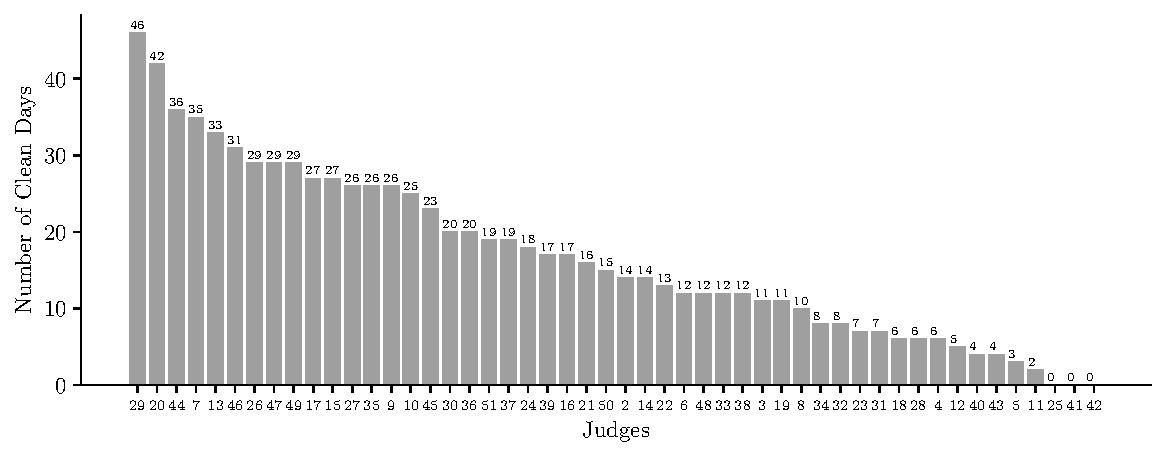
\includegraphics[scale=0.75]{Figures/Judge_Clean_Days_Histogram}
	\vspace{-3mm}
	\caption{The number of "clean" days for each judge.}
	\label{Figure_Judge_Clean_Days_Histogram}
\end{figure}

\subsubsection{Estimation of $\mu_p$}
\label{Sec:Estimation:Capacity_Estimation:Plea_Capacity}
Let $\mathcal{C}_j$ denote the set of "clean" days on judge $j$'s schedule for $j\in\mathcal{J}_p$. Let $S^j_t$ denote the number of pleas observed for judge $j$ on day $t\in\mathcal{C}_j$. Moreover, let $D^j_t$ denote the number of plea cases on judge $j$'s docket on day $t\in\mathcal{C}_j$. Furthermore, let $P^j_t$ denote the number of cases judge $j$ can hear on day $t\in\mathcal{C}_j$. Then, we have $S^j_t = \min(D^j_t,P^j_t)$ for judge $j\in\mathcal{J}_p$ and day $t\in\mathcal{C}_j$. Moreover, we assume $P^j_t \sim \text{Poisson}(\mu_p)$ for judge $j\in\mathcal{J}_p$ and day $t\in\mathcal{C}_j$.\footnote{This assumption holds when the judges spends a fixed number of hours on each working day hearing cases and the time it takes to hear a plea case is exponentially distributed with mean $1/\mu_p$.}

Whenever the number of cases $D^j_t$ is sufficiently large, we have $S^j_t = P^j_t \sim \text{Poisson}(\mu_p)$ for judge $j\in\mathcal{J}_p$ and day $t\in\mathcal{C}_j$. Motivated by this, we choose a cut off value $x$ and focus on the "clean" days during which the judge heard $x$ or more (plea-bargain) cases. The underlying assumption is that $D^j_t$ must have been large enough that on these days, the judge's output is purely determined by his processing rate, i.e., it is not censored by $D^j_t$.

Letting $F$($f$)  denote the cdf (pmf) of a Poisson random variable with mean $\mu_p$, we define the conditional cdf, denoted by $F_x$, as follows:
\begin{align*}
	F_x(k) \,=\, \mathbb{P}\big( P \leq k | P \geq x \big), \quad\quad k\geq x.
\end{align*}
That is,
\begin{align*}
	F_x(k) \,=\, \frac{F(k)-F(x-1)}{1-F(x-1)}, \quad\quad k\geq x.
\end{align*}
We let $f_x$ denote the pmf corresponding to $F_x$, i.e., 
\begin{align*}
	f_x(k) \,=\, \frac{f(k)}{1-F(x-1)}, \quad\quad k \geq x.
\end{align*}
We let $n(x)$ denote the number of "clean" days with $x$ or more sentencing events and define the set 
\begin{align*}
	\mathcal{S}_x \,=\, \{ S^j_t \geq x: j\in\mathcal{J}_p,t\in\mathcal{C}_j \}.
\end{align*}
Note that $\mathcal{S}_x$ has $n(x)$ elements. Then, we define the likelihood of observing the elements in $\mathcal{S}_x$ as follows:
\begin{align*}
	\mathcal{L}_x(\mu_p) \,=\, \prod_{s\in\mathcal{S}_x} f_x(s) \,=\, \prod_{s\in\mathcal{S}_x} \frac{f(s)}{1-F(x-1)}.
\end{align*}
Thus, the log-likelihood is $\log \mathcal{L}_x(\mu_p) \,=\, \sum_{s\in\mathcal{S}_x} \log f(s) - n(x) \log (1-F(x-1))$. We define $\mu^\star_p(x) = \argmax_{\mu_p} \log \mathcal{L}_x(\mu_p)$. Figure \ref{Figure_Plea_Service_Rate_MLE_Estimate} depicts $\mu^\star_p(x)$ as a function of $x$. 
%
\begin{figure}[H]
	\centering
	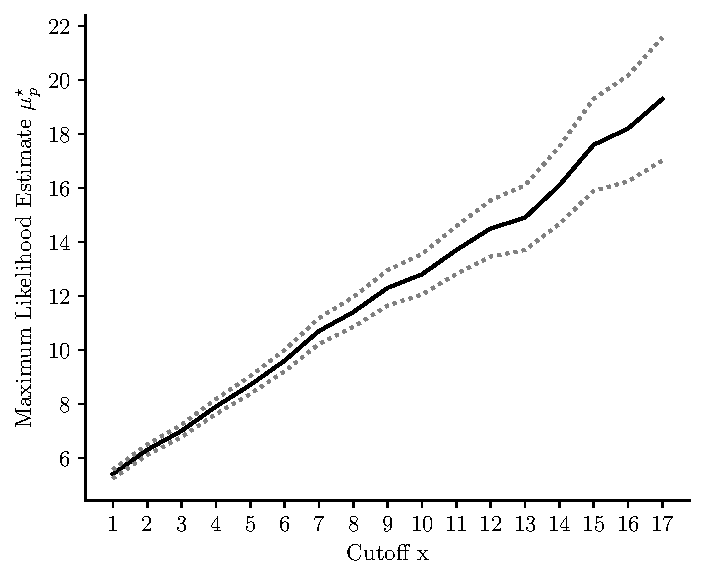
\includegraphics[scale=0.75]{Figures/Likelihood_Estiamtes_Top}
	\vspace{-2mm}
	\caption{The maximum likelihood estimate for the plea service rate as a function of the cutoff value $x$. The solid line depicts the MLE estimate and the dashed lines depict the 95\% confidence interval.}
	\label{Figure_Plea_Service_Rate_MLE_Estimate}
\end{figure}
%
Figure \ref{Figure_Plea_Service_Rate_Log_Likelihood_Per_Observation} depicts the log-likelihood per observation, i.e., $\max_{\mu_p} \log \mathcal{L}_x(\mu_p)/n(x)$ as a function of $x$. We can choose the cutoff value $x$ in a number of ways. Two plausible approaches are as follows:
\begin{itemize}
	\vspace{-1mm}
	\item[(i)] We choose $x = 7$, which corresponds to the 75\% percentile of the number of sentences per day in the sentencing dataset; see Figure \ref{Figure_Sentences_Per_Day_Histogram}. This choice gives us a plea service rate estimate of $\hat{\mu}_p = 10.7$ pleas per day with a standard error of $0.3$ pleas per day.
	\vspace{-1mm}
	%
	\begin{figure}[H]
		\centering
		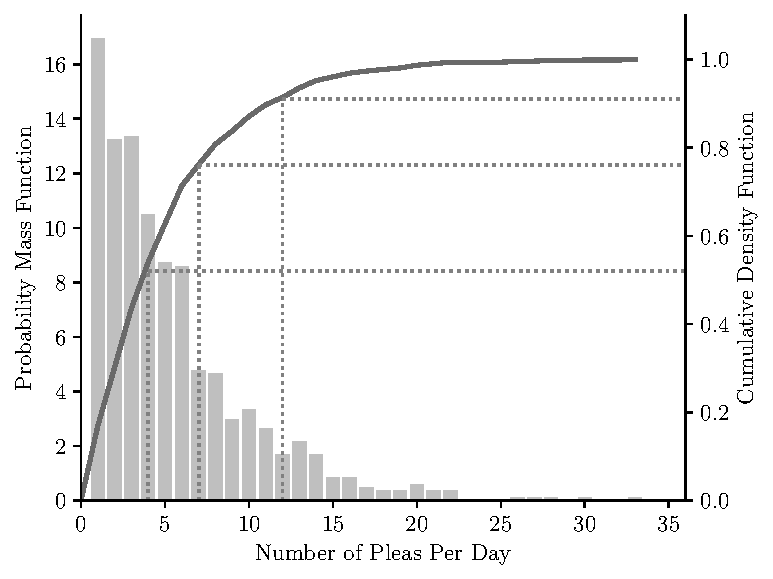
\includegraphics[scale=0.75]{Figures/Histogram_Pleas_Per_Day}
		\vspace{-2mm}
		\caption{The cdf and pmf of the number of sentences per day. The dashed lines depict the 50\%, 75\%, and 95\% percentiles.}
		\label{Figure_Sentences_Per_Day_Histogram}
	\end{figure}
	%
	\item[(ii)] We choose $x = 13$, which is the value of $x$ that achieves the highest $\max_{\mu_p} \log \mathcal{L}_x(\mu_p)/n(x)$, log-likelihood per observation. This choice gives us a plea service rate estimate of $\hat{\mu}_p = 14.9$ plea per day with a standard error of $0.6$ pleas per day.
\end{itemize}
%
\begin{figure}[H]
	\centering
	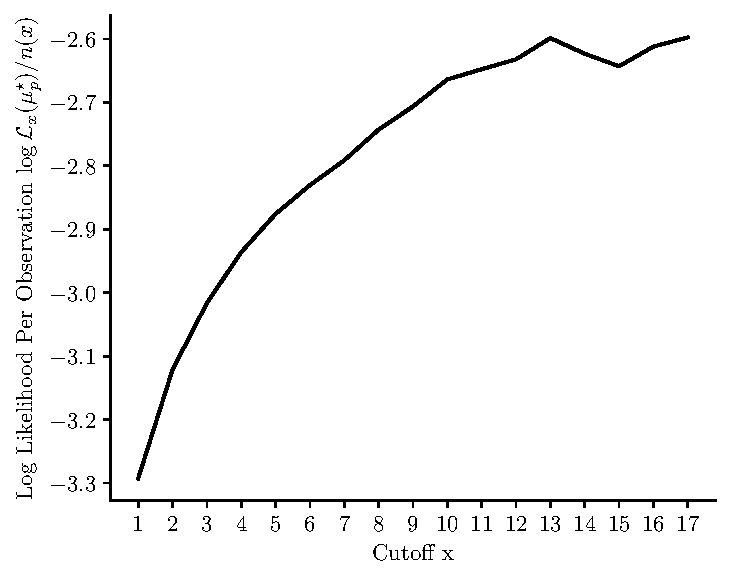
\includegraphics[scale=0.75]{Figures/Log_Likelihood_Per_Observation_Top}
	\caption{The log-likelihood per observation for the plea service rate as a function of the cutoff value $x$.}
	\vspace{-2mm}
	\label{Figure_Plea_Service_Rate_Log_Likelihood_Per_Observation}
\end{figure}
%
In the remainder of this section, for concreteness, we use the first approach, i.e., we assume $\hat{\mu}_p = 10.7$ pleas per day.

\subsubsection{Estimation of $\mu_t$}
To estimate the trial service rate, we focus on the judge-county combinations that satisfy the following conditions:
\begin{enumerate}[label=(\roman*)]
	\vspace{-2mm}
	\item The judge does not undertake more than 35 sentencing events on any day in this county.
	\item The judge has at least one trial in this county. 
\end{enumerate}
\vspace{-1mm}
By focusing on these judge-county combinations, we avoid the outliers (as done in the estimation of the plea service rate) and ensure that the judge spent some of his time processing trials. Let $K$ denote the number judge-county combinations satisfying these two conditions. We number these judge-county combinations $1,\ldots,K$ and define $\mathcal{K} = \{1,\ldots,K\}$. For judge-county $k \in \mathcal{K}$, we let $n_p(k)$ and $n_t(k)$ denote the total number of pleas and the total number of trials undertaken by this judge in this county. Similarly, for judge-county $k \in \mathcal{K}$, we let $T(k)$ denote the number of days this judge was assigned to this county.\footnote{In calculating $T(k)$ for $k\in\mathcal{K}$, we assume the judge divides his time equally among the county assignments to which he is assigned if he is assigned to multiple counties on a day.}

First, we assume the judges in judge-county combinations $k\in\mathcal{K}$ never idle. We will revisit this assumption later. If this assumption was correct, the trial service rate of judge-county $k\in\mathcal{K}$ would be
\begin{align*}
	\hat{\mu}_t(k) \,=\, \frac{n_t(k)}{T(k) - n_p(k) / \hat{\mu}_p}.
\end{align*}
The tuples $(n_t(k),{\hat{\mu}_t(k)})$ for $k\in\mathcal{K}$ are depicted in Figure \ref{Figure_Trial_Sercice_Rate_Vs_Trial_Per_County}.
%
\begin{figure}[H]
	\centering
	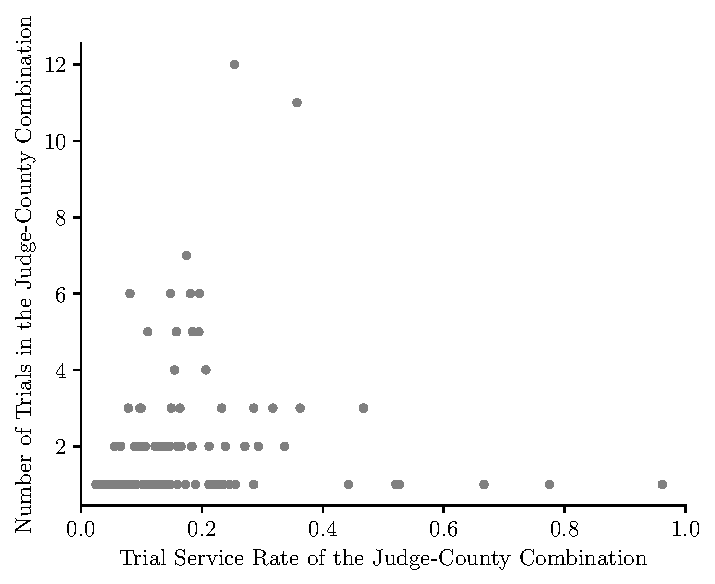
\includegraphics[scale=0.75]{Figures/Judge_Capacity_Vs_Number_of_Trials}
	\vspace{-2mm}
	\caption{A graphical representation of the tuples $(n_t(k),{\hat{\mu}_t(k)})$ for $k\in\mathcal{K}$.}
	\label{Figure_Trial_Sercice_Rate_Vs_Trial_Per_County}
\end{figure}
%
We observe that as the number of trials in a judge-county combination decreases, the variance of the $\hat{\mu}_t(k)$ estimates increase. Moreover, the $\hat{\mu}_t(k)$ estimates skew to the left as the number of trials decreases. This suggests that the judges in judge-county combinations with few trials spent some time idling. Therefore, to estimate the trail service rate, we focus on judge-county combinations for which we observe at least two trials, i.e., $k \in \tilde{\mathcal{K}} = \{k:k\in\mathcal{K},n_t(k)\geq 2\}$. These judge-county combinations account for $72\%$ of the trials in the dataset. The trial service rate estimate is 
%
\begin{align*} 
	\hat{\mu}_t \,=\, \frac{ \sum\limits_{k\in\tilde{\mathcal{K}}} n_t(k) }{\sum\limits_{k\in\tilde{\mathcal{K}}} T(k) - \sum\limits_{k\in\tilde{\mathcal{K}}} n_p(k) / \hat{\mu}_p }.
\end{align*}
%
We obtain a trial service rate estimate of $\hat{\mu}_t = 0.15$ trials per day, i.e., an average trial processing time of $6.6$ days.\footnote{If we focus on judge-county combinations with at least 3 or 4 trials, we obtain a trial processing rates of $0.17$ trials per day. These judge-county combinations account for $49\%$ and $37\%$ of the trials in the dataset, respectively.} Figure \ref{Figure_Trial_Service_Rate_Utilization_Estimate} depicts the utilization estimate, i.e., $\big(n_t(k)/\hat{\mu}_t+n_p(k)/\hat{\mu}_p\big)/T(k)$ for $k\in\hat{\mathcal{K}}$. About $78.84\%$ of the judge-county combinations have a utilization estimate of at least 80\%. Some judge-county combinations have, however, a utilization estimate of 1.5 or higher, which seems suspicious. If we do not include these judge-county combinations in the estimation of the trial service rate, we obtain a service rate estimate of $0.14$ trials per day (an average trial processing time of $7.4$ days).
%
\begin{figure}[H]
	\centering
	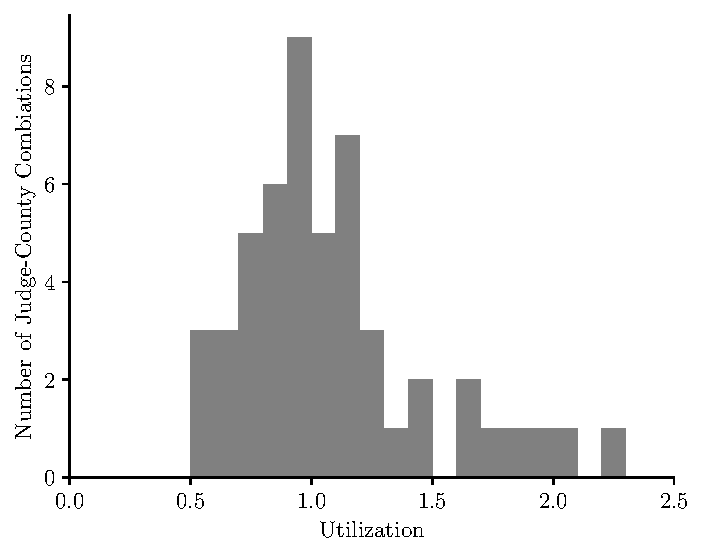
\includegraphics[scale=0.75]{Figures/Utilization_Of_Judge_County_Combiations_Included_Histogram}
	\vspace{-2mm}
	\caption{The utilization estimate of the judge-county combinations $k\in\hat{\mathcal{K}}$.}
	\label{Figure_Trial_Service_Rate_Utilization_Estimate}
\end{figure}

%We focus on the top trial judges (and the busiest judges overall) and the assignments \Blue{during} which he does not split his time across different counties and is only assigned to general session (GS). Let $\mathcal{J}_t$ denote the set of judges we focus on. Focusing on \Blue{the assignments mentioned immediately above,} we estimate $\mu_t$, the service rate of trials per week, as follows: Let $n_p(j)$ denote the total number of pleas judge $j\in\mathcal{J}_t$ handles during the assignments considered and $\tau_j$ denote the number of weeks judge $j$ works for the chosen assignments. Similarly, let $n_t(j)$ denote the number of trials judge $j$ handles. Assuming judges in set $\mathcal{J}_t$ are 100\% busy (with handling plea bargains and trials), we write 
%\begin{align*}
%	\frac{n_p(j)}{\mu_p} + \frac{n_t(j)}{\mu_t} \,=\, \tau_j,\quad\quad j\in\mathcal{J}_t.
%\end{align*}
%Summing over $j$ gives 
%\begin{align*}
%		\frac{\sum\limits_{j\in\mathcal{J}_t}n_p(j)}{\mu_p} + \frac{\sum\limits_{j\in\mathcal{J}_t}n_t(j)}{\mu_t} \,=\, \sum_{j\in\mathcal{J}_t}\tau_j,
%\end{align*}
%which constitutes the key equation for the estimation of $\mu_p$. Substituting $\hat{\mu}_p$ from the estimation procedure described in Section \ref{Sec:Estimation:Capacity_Estimation:Plea_Capacity}, we get 
%\begin{align*}
%	 \hat{\mu}_t \,=\, \frac{ \hat{\mu}_p\sum\limits_{j\in\mathcal{J}_t} n_t(j) }{ \hat{\mu}_p\sum\limits_{j\in\mathcal{J}_t} \tau_j - \sum\limits_{j\in\mathcal{J}_t} n_p(j) }. 
%\end{align*}

\begin{remark}[An alternative $\mu_t$ estimate.]
	Consider judge $j\in\mathcal{J}_t$, who sentenced $n_p(j)$ pleas and $n_t(j)$ trials. The total time pleas take, denoted by $X_p(j)$, is an $\text{Erlang}(n_p(j),\mu_p)$ random variable. Then, the number of trials sentenced by judge $j$ is a Poisson random variable with mean $\mu_t(\tau_j-X_p(j))$. In particular, the likelihood of observing $n_t(j)$ trials is 
	\begin{align*}
		\mathscr{L}_j \,=\, \int_0^{\tau_j} e^{-\mu_t(1-x)} \frac{(\mu_t(1-x))^{n_t(j)}}{n_t(j)!} g_j(x) dx,
	\end{align*} 
	where $g_j$ is the pdf for the $\text{Erlang}(n_p(j),\mu_p)$ random variable. Then, letting $\mathscr{L}=\prod_{j\in\mathcal{J}_t} \mathscr{L}_j$ gives $\hat{\mu}_t=\argmax_{\mu_t} \mathscr{L}$ via MLE.
\end{remark}

\subsubsection{Judge Schedules in the Data}
We plan to use the master calendar whenever there are no conflicts with the sentencing dataset. However, there are some conflicts between the two data sources as reviewed in Section \ref{Sec:Master_Calendar_Description}. In those cases, we propose to proceed as follows: If the number of conflicts is "small", then we stick with the schedule on the master calendar because the conflicts appear negligible. Otherwise, we propose reallocating the judge's capacity according to the sentencing dataset. To be more specific, one type of conflict is that a judge may be sentencing in multiple counties on a day, both in the one that appears on the master calendar as well as in another that does not appear on the master calendar. If the number of sentencing events in both counties is "significant", then we propose to split the judge's capacity across those two locations proportionally (to the number of sentencing events in each location).

Another type of noteworthy conflict between the two data sources is that a judge may have no assignments according to the master calendar, but sentencing events are recorded for him in a county (according to the sentencing dataset). If the number of those sentencing events is significant, we propose to modify the master calendar accordingly, i.e., the judge is assigned to that county. Otherwise, we propose keeping the schedule on the master calendar as is.


\subsection{Choice Model for Judge Shopping}
We propose three closely related candidates for the defendant's choice model for judge shopping that incorporates the capacity constraints. When a defendant with $(\theta\tau,c_d)$ arrives, he looks at the sequence of the available judges along with the likelihoods of getting them. To be specific, we let $\rho_j$ denote the probability of getting judge $j$ upon requesting him.

As discussed earlier, we assume $v=\infty$ so the defendant can choose among the next $r$ judges, but his case may not be heard by the judge he chooses. In that case, the defendant's case is assigned to one of the judges scheduled after his choice. We propose the following three candidates for the choice model:
%
\vspace{-3mm}
\paragraph{Proposal 1.} If the defendant's case cannot be heard by the judge he chose due to capacity constraints, then it is heard by the next judge on the schedule. Suppose the defendant chooses the judge scheduled for the $i$-th week, denoted by judge $j(i)$, who will hear the case with probability $\rho_{j(i)}$. If she does not hear the case, then the next judge, judge $j(i+1)$, hears it. Letting $\mathpzc{U}_j$ denote the defendant's expected utility from the judge scheduled for the $i$-th week, we have that
\begin{align*}
	\mathpzc{U}_i \,=\, \rho_{j(i)} \min \big( \theta\tau+c_d , \mathpzc{u}_{j(i)}(\theta\tau) \big) \,+\, (1-\rho_{j(i)}) \big( \min \big( \theta\tau+c_d , \mathscr{u}_{j(i+1)}(\theta\tau) \big) + d \big).
\end{align*}
Then, the defendant seeks to $\max_{i=1,\ldots,r} \{\mathpzc{U}_i+i d + \epsilon_i\}$, where $\epsilon_i$ is an extreme-value idiosyncratic shock.
%
\vspace{-3mm}
\paragraph{Proposal 2.} If the defendant is rationed, then judge $j(r+1)$ hears the case. This is similar to the previous case. The only difference is that the expected utility of the defendant from choosing the $i$-th judge is 
\begin{align*}
	\mathpzc{U}_i \,=\, \rho_{j(i)} \min \big( \theta\tau+c_d , \mathpzc{u}_{j(r)}(\theta\tau) \big) \,+\, (1-\rho_{j(i)}) \big( \min \big( \theta\tau+c_d , \mathpzc{u}_{j(r+1)}(\theta\tau) \big) + (r-i+1)d \big).
\end{align*}
%
\vspace{-10mm}
\paragraph{Proposal 3.} A more complex alternative which combines the preceding two proposal is to assume that the defendant is sequentially considered for judges $i,i+1,\ldots,r$. If he is rationed out in all steps, then jduge $r+1$ hears the case. In this case, we have that 
\begin{align*}
	\mathpzc{U}_i \,=\, &\rho_{j(i)} \min \big( \theta\tau+c_d , \mathpzc{u}_{j(i)}(\theta\tau) \big) \,+\, (1-\rho_{j(i)}) \rho_{j(i+1)} \big( \min \big( \theta\tau+c_d , \mathpzc{u}_{j(i+1)}(\theta\tau) \big) + d \big) \\
	&\,+\, (1-\rho_{j(i)})(1-\rho_{j(i+1)})\rho_{j(i+2)} \big( \min \big( \theta\tau+c_d , \mathpzc{u}_{j(i+2)}(\theta\tau) \big) + 2d \big) \\
	&\,+\,\ldots\,+\,(1-\rho_{j(i)})(1-\rho_{j(i+1)})\ldots(1-\rho_{j(r)}) \big( \min \big( \theta\tau+c_d , \mathpzc{u}_{j(r+1)}(\theta\tau) \big) + (r-i+1)d \big).
\end{align*}
%
\vspace{-7mm}
\paragraph{Estimation of rationing probabilities $\rho_1,\ldots,\rho_J$.} The easiest approach to estimating the rationing probability appears to be the iterative simulation approach. We start with an initial guess $\rho^0$. Then, we simulate the allocations and compute $\rho^1$. We iterate until $\rho^n = (\rho_1^n,\ldots,\rho_J^n)$ converges.
\begin{remark}
	We can probably write down equilibrium flow equations. They will likely be too complex. 
\end{remark}
\begin{remark}
	On the one hand, one may consider having the rationing probabilities depend on both the judge and the county, but that may lead to too many parameters. On the other hand, if we find that even $\rho_1,\ldots,\rho_J$ are too many parameters to tune, we may consider grouping the judges with respect to their harshness and estimating a parameter for each group.
\end{remark}

The rest of this section is intended solely to facilitate discussion.
%
\subsection{Simulation Study Outline} 
%
\vspace{-1mm}
\paragraph{Defendant Arrival Process.} For each county, assuming a stationary arrival process (which can be relaxed), we can calculate a (weekly) arrival rate and generate arrivals from a Poisson process with that rate. When an arrival occurs, we pick a defendant from the dataset at random (with replacement) who is sentenced in that county.
%
\vspace{-3mm}
\paragraph{State Variable for the Simulation.} The state variable is the judge's dockets, i.e., the cases assigned to each judge (in each county) currently, as well as their remaining capacity for each of the following weeks. We may want to keep track of it continuously. We also assume the judge schedules are given so we can determine where they are each week and which cases they can hear.

\begin{remark}
	Perhaps, we can get away with just the remaining capacity of the judges over the next $r+1$ weeks, depending on whether plea/trial processing times are deterministic and how we model trials.
\end{remark}

\begin{question}
	Should we model the number of cases a judge can handle per day deterministically or randomly?
\end{question}
This interacts with the way the case assignments are made. Perhaps, we can assume the plea-bargain processing is deterministic, because they likely take a simple interaction with the judge. Also, having it deterministic will simplify the way we assign the cases to judges and the way we keep track of the judges' remaining capacity in the future. However, trials may take multiple (and longer) court visits.
%
\vspace{-3mm}
\paragraph{How Should We Model Trials in the Simulation?} Could we decide the duration and the number of court visits
upon arrival and book those on the judge's schedule?
%
\begin{note}
	Larry's guidance will be most helpful here.
\end{note}
%
\vspace{-3mm}
\paragraph{Calibration.} Once the details of the simulation are decided, we can simulate the above model to calibrate the values of $d$ (the cost of delaying by a week) and $r$ (the maximum delay a defendant can choose) so as to match some key performance metrics in the data. We can then use it for the counterfactual analysis.
%
\subsection{Counterfactual Study}
This section will study the effects of $r$, $d$, and most importantly, the judge rotations. To that end, we can consider alternative judge schedules, and perhaps look for the "optimal" judge rotation. What are some reasonable benchmarks?
\begin{itemize}
	\vspace{-3mm}
	\item[a)] All judges are available every week (perhaps virtually)
	\item[b)] Judges are assigned uniformly (perhaps at random).
	\item[c)] What else?
	\vspace{-3mm}
\end{itemize}
Given $d$, $r$, and a new judge sequence, we can iteratively simulate the system to get the equilibrium judge availabilities, i.e., $\rho_1,\ldots,\rho_J$. Once the simulation converges, we can compute/report the counterfactual results.
%
\vspace{-3mm}
\paragraph{What Should We Report?} Here are some possibilities: Sentence length distributions conditional
on $\hat{\theta}\hat{\tau}$, e.g., $\mathbb{E}\big[ \text{Sentence Length}\big| \hat{\theta}\hat{\tau} \big]$ and $\text{Var}\big[ \text{Sentence Length}\big| \hat{\theta}\hat{\tau} \big]$. It may also be interesting to document before-after comparisons across different counties, under a new judge rotation. In addition, we can report the changes in the number of pleas vs. trials each judge handles.
%
\begin{question}
	What else would be helpful to report?
\end{question}


\section{Additional Questions}
\label{Sec:Questions}

This section presents the questions we have on the datasets (and their interpretations) discussed in the previous section.

\begin{question}
	What do the counts, sgc\_offcode, ccpnts, and ppoints data fields of the CSV file correspond to?
\end{question}

\begin{question}
	The mapping from offser numbers to felony classes is not monotone in felony classes. Is this correct?
\end{question}

\begin{question}
	Are the judges only engaged in the assignments stated on the master calendar or they have other duties (that may take a considerable amount of their time), as well?
\end{question}

\bibliographystyle{plainnat}
\bibliography{bibfile}

\clearpage
\appendix

\section{Data Cleaning}
\label{Sec:Appendix:Data_Cleaning}
This section describes the steps taken to clean our datasets, i.e., the sentencing dataset (the CSV file) and the master calendar:
\begin{enumerate}
	\item We discard all sentencing events in the sentencing dataset associated with Judge 1 because Judge 1 is a fictitious judge.\footnote{See the email from Rhys to Can and Larry on 05/14/2018 (Page 3 of the document Email3.pdf). In this email, Rhys states that "Judge 1 is actually a fictitious aggregate of the 155 cases that were missing a judge ID".}
	\item We discard all judge names that are not mapped to a judge number from the master calendar. Because, we do not observe any sentencing events for these judges in the sentencing dataset. These judge names are as follows: Bergdorf, Couch, Drew, Gier, Peeples, Simmons, Watts, and Young. It appears that since \citet{Hester_Hartman_2017} uses a similar sentencing dataset, it does not include these judges in its analysis, either.
	\item We combine (the schedules of) Judges Cooper and Cooper, TW in the master calendar. There are three judges on the master calendar with last name Cooper: (i) Cooper, (ii) Cooper, TW, and (iii) Cooper, GT. If we run the algorithm proposed in Section \ref{Sec:Mapping_Judge_Numbers_To_Judge_Names} using the master calendar with three distinct judges with last name Cooper, Judge 14 is mapped to either Judge Cooper (under the perfect match criterion) or Judge Cooper, TW (under the overlapping match criterion). Table \ref{Table_Coopers_Schedules} depicts the schedules of the three judges with last name Cooper (according to the master calendar) as well as the counties visited by Judge 14 (according to the sentencing dataset). The counties to which either Judge Cooper or Judge Cooper, TW are assigned are depicted in blue. The counties to which Judge Cooper, GT is assigned are depicted in green. The counties to which neither Judge Cooper, nor Judge Cooper, TW or Cooper, GT are assigned are depicted in red. Table \ref{Table_Coopers_Schedules} shows that the schedules of Judges Cooper and Cooper, TW do not overlap. Moreover, their combined schedules resemble the schedule of Judge 14 (the list of counties visited by Judge 14) the most. This suggests that Judge Cooper and Judge Cooper, TW are (most likely) the same person. Therefore, we combine the schedules of Judges Cooper and Cooper, TW.\footnote{Incidentally, only two judges with last name Cooper are listed on the South Carolina Judicial branch's website. These judges are Thomas W. Cooper, Jr. and G. Thomas Cooper, Jr.; please see \url{https://www.sccourts.org/circuitCourt/displaycirjudge.cfm?judgeid=2054} and \url{https://www.sccourts.org/circuitCourt/displaycirjudge.cfm?judgeid=2126} (accessed on December 14th, 2020) for their bios.}
\end{enumerate}
%\begin{note}
%	Baris postulated that the sentencing events undertaken by these seven judges were deleted from the sentencing dataset by Rhys. However, I could not find a reference to this hypothesis in Rhy's emails. In fact, on page 3 of the document Email3.pdf, Rhys states that "Judge 1 is actually a fictitious aggregate of the 155 cases that were missing a judge ID". This seems to suggest that Rhy did not delete any judge numbers/names. In fact, this statement suggests that the dataset Rhys obtained was already missing this information. Moreover, Table \ref{Table_Schedule_Of_Unmapped_Judge_Names} shows that there is very little overlap between the set of counties visited by Judge 1 and the set of counties visited by the remaining seven judge names. Therefore, we can not claim that Judge 1 is a combination of the remaining seven judges.
%\end{note}}

\begin{table}[H]
	\centering
	\vspace{-11mm}
	\hspace*{-16mm}
	\setlength\tabcolsep{0pt} % default value: 6pt
	{\footnotesize
		\begin{tabular}{L{23mm}C{55mm}C{38mm}C{38mm}C{38mm}}
			\toprule
			\rule{0pt}{2.3ex} Week & Judge 14 & Cooper & Cooper, TW & Cooper, GT \\
			\midrule
			%\rowgroup{Consumer Surplus} \\
			%\rule{0pt}{2.3ex} July 3 & & & &\\
			\rule{0pt}{2.3ex} July 10 & & \textcolor{black}{Aiken} & &\\
			\rule{0pt}{2.3ex} July 17 & & & &  \textcolor{black}{Berkeley}\\\rule{0pt}{2.3ex} July 24 & & & &  \textcolor{black}{Richland}\\
			\rule{0pt}{2.3ex} July 31 & & \textcolor{black}{Sumter} & &  \textcolor{black}{Greenville}\\\rule{0pt}{2.3ex} August 7 &  \textcolor{green}{Sumter} & \textcolor{green}{Sumter} & &  \textcolor{black}{Greenwood}\\
			\rule{0pt}{2.3ex} August 21 &  \textcolor{blue}{Greenville} & \textcolor{black}{Sumter} & &  \textcolor{blue}{Greenville}\\
			\rule{0pt}{2.3ex} August 28 &  \textcolor{green}{Williamsburg}, \textcolor{red}{Sumter} & \textcolor{green}{Williamsburg}, \textcolor{black}{Orangeburg} & &  \textcolor{black}{Richland}, \textcolor{black}{Greenville}\\
			\rule{0pt}{2.3ex} September 4 &  \textcolor{green}{Williamsburg}, \textcolor{blue}{Greenville} & \textcolor{green}{Williamsburg} & &  \textcolor{blue}{Greenville}\\
			\rule{0pt}{2.3ex} September 11 &  \textcolor{green}{Sumter}, \textcolor{red}{Clarendon}, \textcolor{blue}{Greenville} & \textcolor{green}{Sumter} & &  \textcolor{blue}{Greenville}\\
			\rule{0pt}{2.3ex} September 18 & & & &  \textcolor{black}{Spartanburg}\\
			\rule{0pt}{2.3ex} September 25 &  \textcolor{blue}{Greenville} & \textcolor{black}{Williamsburg} & &  \textcolor{blue}{Greenville}\\
			\rule{0pt}{2.3ex} October 9 &  \textcolor{green}{Lee}, \textcolor{red}{Sumter} & \textcolor{green}{Lee} & &  \textcolor{black}{Richland}\\
			\rule{0pt}{2.3ex} October 16 &  \textcolor{green}{Williamsburg} & \textcolor{green}{Williamsburg}, \textcolor{black}{Aiken} & &  \textcolor{black}{Richland}\\
			\rule{0pt}{2.3ex} October 23 &  \textcolor{green}{Williamsburg}, \textcolor{red}{Horry}, \textcolor{red}{Georgetown} & \textcolor{green}{Williamsburg} & &\\
			\rule{0pt}{2.3ex} October 30 &  \textcolor{green}{Sumter} & \textcolor{green}{Sumter} & &  \textcolor{black}{Richland}\\
			\rule{0pt}{2.3ex} November 6 & & \textcolor{black}{Williamsburg} & &  \textcolor{black}{Richland}\\\rule{0pt}{2.3ex} November 13 &  \textcolor{green}{Sumter} & \textcolor{green}{Sumter} & &\\
			\rule{0pt}{2.3ex} November 27 & & \textcolor{black}{Clarendon} & &  \textcolor{black}{Newberry}\\
			\rule{0pt}{2.3ex} December 4 &  \textcolor{green}{Lee}, \textcolor{red}{Sumter} & \textcolor{green}{Lee} & &\\
			\rule{0pt}{2.3ex} December 11 &  \textcolor{green}{Lee} & \textcolor{green}{Lee}, \textcolor{black}{Aiken} & &\\
			\rule{0pt}{2.3ex} January 1 & & & \textcolor{black}{Aiken} &\\
			\rule{0pt}{2.3ex} January 8 &  \textcolor{green}{Richland} & & \textcolor{green}{Richland}, \textcolor{black}{Aiken} &  \textcolor{black}{McCormick}\\
			\rule{0pt}{2.3ex} January 15 & & & \textcolor{black}{Kershaw} &\\
			\rule{0pt}{2.3ex} January 22 & & & \textcolor{black}{Aiken} &\\
			\rule{0pt}{2.3ex} January 29 &  \textcolor{green}{Aiken} & & \textcolor{black}{Beaufort}, \textcolor{green}{Aiken} &  \textcolor{black}{Lexington}\\
			\rule{0pt}{2.3ex} February 5 & & & \textcolor{black}{Orangeburg} &  \textcolor{black}{Laurens}\\
			\rule{0pt}{2.3ex} February 12 & & & &  \textcolor{black}{Newberry}\\
			\rule{0pt}{2.3ex} February 26 &  \textcolor{green}{Richland} & & \textcolor{green}{Richland}, \textcolor{black}{Orangeburg} &  \textcolor{black}{Greenville}\\
			\rule{0pt}{2.3ex} March 5 &  \textcolor{red}{Richland}, \textcolor{blue}{Edgefield} & & &  \textcolor{black}{McCormick}, \textcolor{blue}{Edgefield}\\
			\rule{0pt}{2.3ex} March 12 & & & \textcolor{black}{Orangeburg} &\\
			\rule{0pt}{2.3ex} March 19 &  \textcolor{green}{Orangeburg} & & \textcolor{green}{Orangeburg} &\\
			\rule{0pt}{2.3ex} March 26 &  \textcolor{green}{Richland} & & \textcolor{green}{Richland} &  \textcolor{black}{Edgefield}\\
			\rule{0pt}{2.3ex} April 9 &  \textcolor{green}{Richland} & & \textcolor{green}{Richland} &  \textcolor{black}{Lexington}\\
			\rule{0pt}{2.3ex} April 16 &  \textcolor{red}{Richland} & & &\\
			\rule{0pt}{2.3ex} April 23 & & & \textcolor{black}{Richland} &  \textcolor{black}{Lexington}\\
			\rule{0pt}{2.3ex} April 30 &  \textcolor{green}{Kershaw} & & \textcolor{green}{Kershaw} &  \textcolor{black}{Lexington}\\
			\rule{0pt}{2.3ex} May 14 & & & &  \textcolor{black}{Lexington}\\\rule{0pt}{2.3ex} May 21 &  \textcolor{green}{Richland} & & \textcolor{green}{Richland} &  \textcolor{black}{Edgefield}\\
			\rule{0pt}{2.3ex} May 28 &  \textcolor{green}{Richland} & & \textcolor{green}{Richland} &\\
			\rule{0pt}{2.3ex} June 4 &  \textcolor{green}{Richland} & & \textcolor{green}{Richland} &  \textcolor{black}{Edgefield}\\
			\rule{0pt}{2.3ex} June 11 & & & &  \textcolor{black}{Edgefield}\\\rule{0pt}{2.3ex} June 18 &  \textcolor{green}{Kershaw} & & \textcolor{green}{Kershaw} &  \textcolor{black}{Lexington}\\
			\rule{0pt}{2.3ex} June 25 & & & \textcolor{black}{Richland} &  \textcolor{black}{McCormick}\\
			\bottomrule
		\end{tabular}
	}
	\vspace{-1mm}
	\caption{The list of counties visited by Judge 14 (according to the sentencing dataset) and the counties visited by Judges Cooper, Cooper, TW, and Cooper, GT (according to the master calendar). The counties visited by Judge 14 to which either Judge Cooper or Judge Cooper, TW were assigned are written in green font. The counties visited by Judge 14 to which Judge Cooper, GT was assigned are written in blue font. The counties visited by Judge 14 to which neither Judge Cooper, nor Judge Cooper, TW or Cooper, GT were assigned are written in red font. For visual clarity, only the weeks in which at least one judge has an assignment or sentencing event are depicted.}
	\label{Table_Coopers_Schedules}
	\vspace{-2mm}
\end{table}

\section{Supplementary Material}
\label{Sec:Appendix:Supplementary_Material}
This section provides supplementary tables in Appendix \ref{Sec:Appendix:Supplementary_Tables} and supplementary figures in Appendix \ref{Sec:Appendix:Supplementary_Figures}.

\subsection{Tables}
\label{Sec:Appendix:Supplementary_Tables}
\vspace{5mm}

\begin{table}[H]
	\centering
	\caption{Some examples of the non-identical statute entries in the CSV and STATA files.} 
	\vspace{-2mm}
	\setlength\tabcolsep{8pt} % default value: 6pt
	{\footnotesize
		\begin{tabular}{L{70mm}L{70mm}}
			\toprule
			CSV File &  STATA File \\
			\midrule
			%\rowgroup{Consumer Surplus} \\
			Grand Larceny, Value \$5,000 or More &
			Grand Larceny, Value \$5,000 or MoreLarceny/Grand, \$5,000/more \\
			& \\
			Breaking into Motor Vehicle or Tanks, Pumps, where Fuel, Lubricants Stored &
			Breaking into Motor Vehicle or Tanks, Pumps, where Fuel, Lubricants StoredLarceny/Break into vehicle/fuel tanks, etc \\
			& \\
			Property Offense, 3rd or Subsequent Conviction, Enhancement to Felony E &
			Property Offense, 3rd or Subsequent Conviction, Enhancement to Felony EEnhancement/Prop off, 3rd/sb conv, Fel E\\
			\bottomrule
		\end{tabular}
	}
	\label{Table_Sentencing_Data_Fields_Statute}
\end{table}

\begin{table}[H]
	\centering
	\caption{Some examples of the non-identical offdescr entries in the CSV and STATA files.} 
	\vspace{-2mm}
	\setlength\tabcolsep{8pt} % default value: 6pt
	{\footnotesize
		\begin{tabular}{L{70mm}L{70mm}}
			\toprule
			CSV File &  STATA File \\
			\midrule
			%\rowgroup{Consumer Surplus} \\
			Assault and Battery of a High and Aggravated Nature (ABHAN) &
			Assault and Battery of a High and Aggravated Nature (ABHAN)Malicious/Inj to animal, >\$1000 < \$5000 \\
			& \\
			Burglary (Non - Violent)  (After June 20, 1985) - 2nd DegreeBurglary/(Non-V)(After 1/20/85)-2nd degree
			& Burglary (Non - Violent)  (After June 20, 1985) - 2nd Degree \\
			& \\
			Possession of Narcotic in Schedule I(b),(c),LSD \& Schedule II (Cocaine)- 1st Offense*Drugs/Poss < 1 gm of ice crank c/c-1st & Possession of Narcotic in Schedule I(b),(c),LSD \& Schedule II (Cocaine)- 1st Offense \\
			& \\
			\bottomrule
		\end{tabular}
	}
	\label{Table_Sentencing_Data_Fields_Offdescr}
\end{table}	

\begin{table}[H]
	\centering
	\caption{County composition of circuit courts.} 
	\vspace{0mm}
	\setlength\tabcolsep{8pt} % default value: 6pt
	{\footnotesize
		\begin{tabular}{C{10mm}L{70mm}}
			\toprule
			Circuit & Counties  \\
			\midrule
			%\rowgroup{Consumer Surplus} \\
			1 & Calhoun, Dorchester, Orangeburg \\
			2 & Aiken, Bamberg, Barnwell \\
			3 & Clarendon, Lee, Sumter, Williamsburg \\
			4 & Chesterfield, Darlington, Dillon, Marlboro,  \\
			5 & Kershaw, Richland \\
			6 & Chester, Fairfield, Lancaster \\
			7 & Cherokee, Spartanburg \\
			8 & Abbeville, Greenwood, Laurens, Newberry  \\
			9 & Berkeley, Charleston \\
			10 & Anderson, Oconee \\
			11 & Edgefield, Lexington, McCormick, Saluda  \\
			12 & Florence, Marion \\
			13 & Greenville, Pickens \\
			14 & Allendale, Beaufort, Colleton, Hampton, Jasper \\
			15 & Horry, Georgetown \\
			16 & Union, York \\
			\bottomrule
		\end{tabular}
	}
	\label{Table_Circuit_Court_Counties}
\end{table}

\begin{table}[H]
	\centering
	\caption{The mapping from the judge numbers to the judge names.} 
	\vspace{-2mm}
	\setlength\tabcolsep{0pt} % default value: 6pt
	{\footnotesize
		\begin{tabular}{>{\quad}C{25mm}C{35mm}|C{28mm}C{30mm}}
			\toprule
			Judge Number & Judge Name & Judge Number & Judge Name \\
			\midrule
			2 & ALFORD & 27 & JOHNSON \\
			3 & BARBER & 28 & KEESLEY \\
			4 & BAXLEY & 29 & KINARD \\
			5 & BEATTY & 30 & KING \\
			6 & BREEDEN & 31 & KITTREDGE \\
			7 & BROGDON & 32 & LEE \\
			8 & BROWN & 33 & LOCKEMY \\
			9 & BUCKNER & 34 & MACAULAY \\
			10 & BURCH & 35 & MANNING \\
			11 & CLARY & 36 & MARTIN \\
			12 & COLE & 37 & MCKELLAR \\
			13 & COOPER, GT & 38 & MILLING \\
			14 & COOPER, TW & 39 & NEWMAN \\
			15 & COTTINGHAM & 40 & NICHOLSON \\
			16 & DENNIS & 41 & PATTERSON \\
			17 & FEW & 42 & PIEPER \\
			18 & FLOYD, H. & 43 & PYLE \\
			19 & FLOYD, S. & 44 & RAWL \\
			20 & GOODE & 45 & SAUNDERS \\
			21 & GOODSTEIN & 46 & SHORT \\
			22 & GREGORY & 47 & SMOAK \\
			23 & HALL & 48 & THOMAS \\
			24 & HARWELL & 49 & WATSON \\
			25 & HAYES & 50 & WESTBROOK \\
			26 & HUGHSTON & 51 & WILLIAMS \\
			\bottomrule
		\end{tabular}
	}
	\label{Table_Mapping_Judge_Numbers_To_Judge_Names}
\end{table}

\begin{table}[H]
	\centering
	\vspace{-5mm}
	\hspace*{-15mm}
	\setlength\tabcolsep{0pt} % default value: 6pt
	{\scriptsize
		\begin{tabular}{L{23mm}C{55mm}C{16mm}C{20mm}C{16mm}C{15mm}C{15mm}C{26mm}C{8mm}}
			\toprule 
			\rule{0pt}{2.3ex} Week & Judge 1 & PEEPLES & BERGDORF & WATTS & YOUNG & COUCH & SIMMONS & GIER \\
			\midrule
			%\rowgroup{Consumer Surplus} \\
			July 3 & & & & & & & &\\
			July 10 &  Greenville, Horry, Richland & \textcolor{red}{Barnwell} & & & & &  \textcolor{blue}{Greenville} &\\
			July 17 &  Anderson, Richland & & & & & & &\\
			July 24 &  York, Richland & & &  \textcolor{red}{Dorchester} & & &  \textcolor{red}{Greenville} &  \textcolor{blue}{York} \\
			July 31 & & \textcolor{red}{Aiken} & & & & &  \textcolor{red}{Greenville} &\\
			August 7 &  York & & & & & & &  \textcolor{blue}{York} \\
			August 14 & & & \textcolor{red}{Orangeburg} & & & & &\\
			August 21 &  Richland, Anderson, York & & & & & & &  \textcolor{blue}{York} \\
			August 28 &  Richland, Kershaw & \textcolor{red}{Aiken} & & & &  \textcolor{red}{Cherokee} &  \textcolor{red}{Greenville} &\\
			September 4 &  Richland & & & & & & &\\
			September 11 &  Greenville & & \textcolor{red}{Orangeburg} &  \textcolor{red}{Dorchester} & & & &  \textcolor{red}{York} \\
			September 18 & & \textcolor{red}{Barnwell} & &  \textcolor{red}{Dorchester} & & & &\\
			September 25 & & & & & & &  \textcolor{red}{Pickens} &  \textcolor{red}{York} \\
			October 2 &  Pickens & & &  \textcolor{red}{Dorchester} & & &  \textcolor{blue}{Pickens}, \textcolor{red}{Greenville} &\\
			October 9 &  York, Richland & \textcolor{red}{Bamberg} & & & & & &  \textcolor{blue}{York} \\
			October 16 &  Richland, Cherokee, Greenville & & &  \textcolor{red}{Dorchester} & &  \textcolor{blue}{Cherokee} & &\\
			October 23 &  Greenville, Spartanburg, Horry & & & & & & &  \textcolor{red}{York} \\
			October 30 &  Richland & \textcolor{red}{Aiken} & & & & &  \textcolor{red}{Greenville} &\\
			November 6 &  Horry & \textcolor{red}{Aiken} & & & & &  \textcolor{red}{Greenville} &  \textcolor{red}{York} \\
			November 13 & & & & & & & &\\
			November 20 & & & & & & &  \textcolor{red}{Greenville} &\\
			November 27 &  Darlington, Spartanburg & & &  \textcolor{red}{Dorchester} & &  \textcolor{red}{Cherokee} &  \textcolor{red}{Greenville} &\\
			December 4 &  Greenville, Richland, Horry & & \textcolor{red}{Orangeburg} & & & & &\\
			December 11 & & & & & & &  \textcolor{red}{Greenville} &  \textcolor{red}{York} \\
			December 18 & & & & & & &  \textcolor{red}{Greenville} &\\
			December 25 & & & & & & & &\\
			January 1 & & & & & & &  \textcolor{red}{Greenville} &\\
			January 8 &  York, Charleston & & & & & & &  \textcolor{blue}{York} \\
			January 15 &  Richland & \textcolor{red}{Aiken} & & &  \textcolor{red}{Chester} & & &\\
			January 22 & & \textcolor{red}{Aiken} & & & & &  \textcolor{red}{Greenville} &  \textcolor{red}{York} \\
			January 29 &  Richland & \textcolor{red}{Aiken} & & &  \textcolor{red}{Chester} &  \textcolor{red}{Cherokee} &  \textcolor{red}{Greenville} &\\
			February 5 &  York, Greenville & & & & & & &  \textcolor{blue}{York} \\
			February 12 &  Greenville, Richland & \textcolor{red}{Bamberg} & & &  \textcolor{red}{Charleston} & & &\\
			February 19 & & & & &  \textcolor{red}{Charleston} & & &  \textcolor{red}{York} \\
			February 26 & & \textcolor{red}{Barnwell} & &  \textcolor{red}{Dorchester} &  \textcolor{red}{Charleston} & &  \textcolor{red}{Greenville} &\\
			March 5 &  Greenville & & & & & & &  \textcolor{red}{York} \\
			March 12 &  Greenville & & & &  \textcolor{red}{Charleston} & & &\\
			March 19 &  Charleston & \textcolor{red}{Aiken} & & & & & &  \textcolor{red}{York} \\
			March 26 &  Charleston & \textcolor{red}{Aiken} & & & & & &\\
			April 2 & & & & &  \textcolor{red}{Charleston} & &  \textcolor{red}{Greenville} &\\
			April 9 &  Spartanburg, Richland & & & &  \textcolor{red}{Charleston} & & &\\
			April 16 &  Spartanburg, Charleston, Greenville, Lee & \textcolor{red}{Aiken} & & &  \textcolor{blue}{Charleston} & & &\\
			April 23 &  Florence, Richland & \textcolor{red}{Aiken} & & & & &  \textcolor{red}{Greenville} &  \textcolor{red}{York} \\
			April 30 &  Richland, Charleston & \textcolor{red}{Aiken} & &  \textcolor{red}{Dorchester} &  \textcolor{blue}{Charleston} & &  \textcolor{red}{Greenville} &\\
			May 7 & & \textcolor{red}{Lancaster} & & &  \textcolor{red}{Charleston} & &  \textcolor{red}{Greenville} &  \textcolor{red}{York} \\
			May 14 &  Florence & & & & & & &\\
			May 21 &  Greenville & \textcolor{red}{Bamberg} & & &  \textcolor{red}{Charleston} & & &  \textcolor{red}{York} \\
			May 28 &  Charleston & \textcolor{red}{Orangeburg} & & & & & &\\
			June 4 &  Richland, Sumter & & & &  \textcolor{red}{Charleston} & & &\\
			June 11 &  Spartanburg, Horry, Greenville, Richland & \textcolor{red}{Aiken} & & &  \textcolor{red}{Charleston} & & &  \textcolor{red}{York} \\
			June 18 &  Richland, Greenville, Charleston & \textcolor{red}{Aiken} & & & & & &\\
			June 25 &  Charleston & \textcolor{red}{Aiken} & &  \textcolor{red}{Dorchester} & &  \textcolor{red}{Cherokee} &  \textcolor{red}{Greenville} &  \textcolor{red}{York} \\
			\bottomrule
		\end{tabular}
	}
	\caption{The schedule of the unmapped judge names. The assignments that coincide with judge 1's schedule are written in blue font. The remaining assignments are written in red font.}
	\label{Table_Schedule_Of_Unmapped_Judge_Names}
\end{table}

\clearpage

\subsection{Figures}
\label{Sec:Appendix:Supplementary_Figures}
This section provides supplementary figures for the main body. In the histograms provides below, the left axis corresponds to the number of sentencing events corresponding to each bar. The right axis corresponds to the percentage of sentencing events correspond to each bar. The counts, ccpnts, ppoints, sentence/realsent, and expmin data fields have a wide range of values. For visual clarity, the figures provided in this section focus on a smaller range of values that encompass 99\% of the sentencing events.
	
\begin{figure}[H]
	\centering
	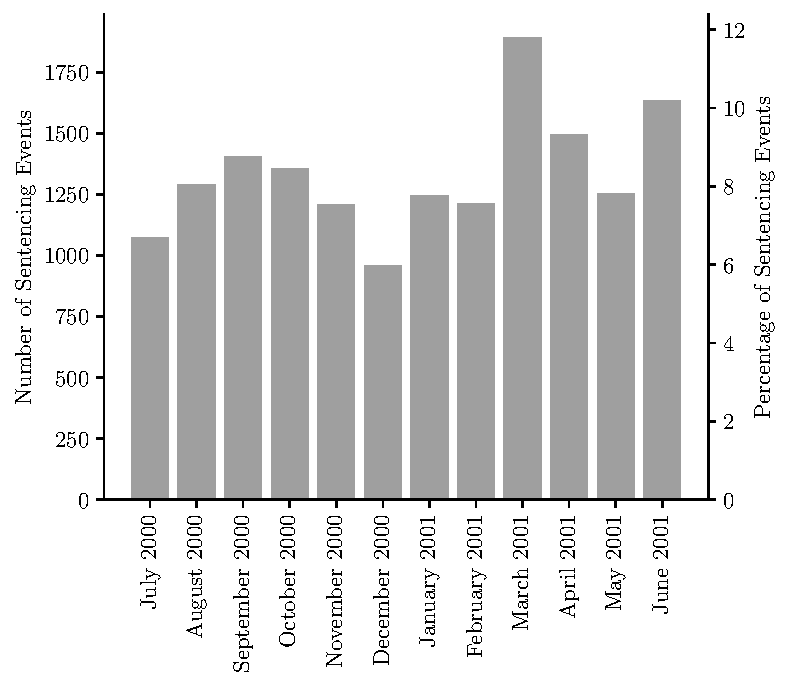
\includegraphics[scale=0.75]{Figures/Month_Histogram}
	\vspace{-2mm}
	\caption{A histogram of the sentencing months.}
	\label{Figure_Hester_Data_Month_Histogram}
\end{figure}
%
\begin{figure}[!]
	\centering
	\begin{minipage}{\textwidth}
		\vspace{-12mm}
		\centering
		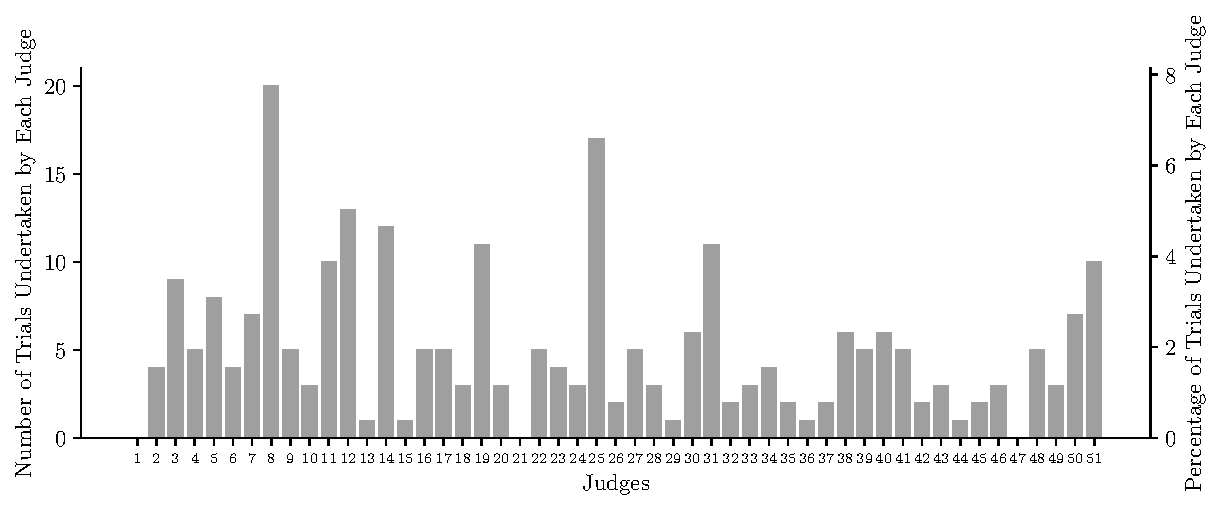
\includegraphics[scale=0.75]{Figures/Trial_Judge_Histogram}
		\vspace{-3mm}
		\caption{A histogram of the trials undertaken by each judge.}
		\label{Figure_Hester_Data_Trial_Judge_Histogram}
	\end{minipage}
	\begin{minipage}{\textwidth}
		\centering
		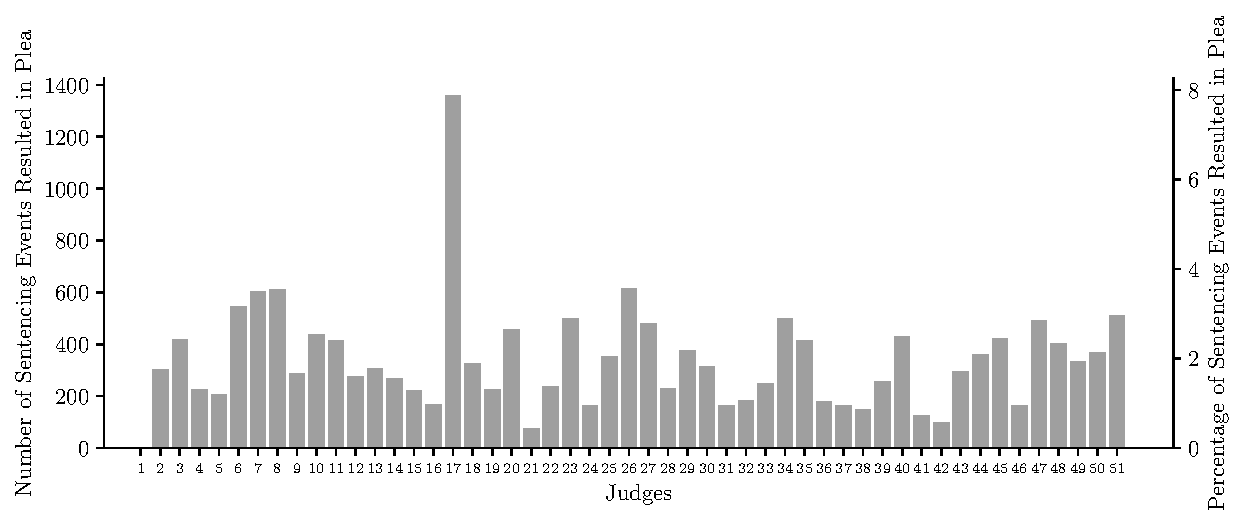
\includegraphics[scale=0.75]{Figures/Judge_Plea_Histogram}
		\vspace{-3mm}
		\caption{A histogram of the pleas for each judge.}
		\label{Figure_Hester_Data_Judge_Plea_Histogram}
	\end{minipage}
	\begin{minipage}{\textwidth}
		\centering
		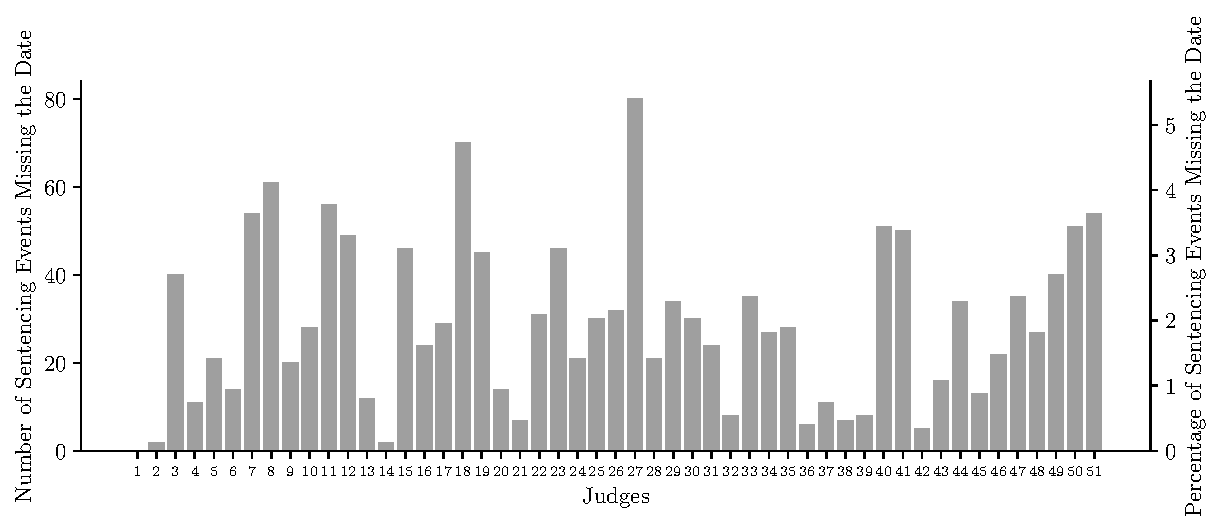
\includegraphics[scale=0.75]{Figures/Missing_Date_Judge_Histogram}
		\vspace{-3mm}
		\caption{A histogram of the sentencing events missing the date data field for each judge.}
		\label{Figure_Hester_Data_Judge_Missing_Date_Histogram}
	\end{minipage}
\end{figure}
%
\begin{figure}[h!]
	\centering
	\hspace*{-18mm}
	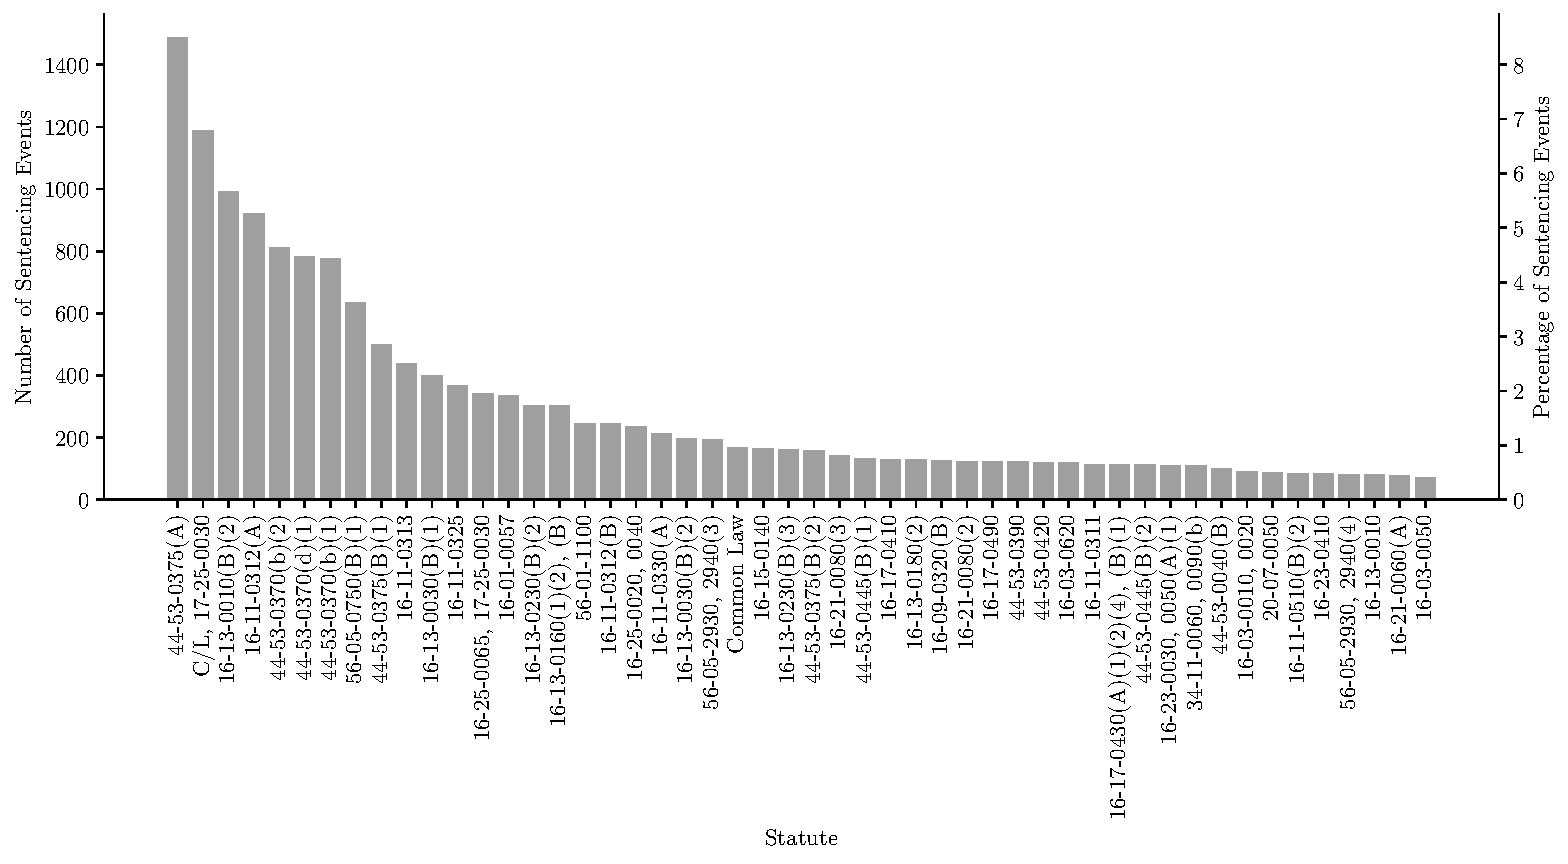
\includegraphics[scale=0.75]{Figures/statute_first_Histogram}
	\vspace{-2mm}
	\caption{A histogram of the statute entries. There are 253 distinct entries. For visual clarify, this figure focuses on the 30 most commons statutes.}
	\label{Figure_Statute_Histogram}
\end{figure}
%
\begin{figure}[h!]
	\centering
	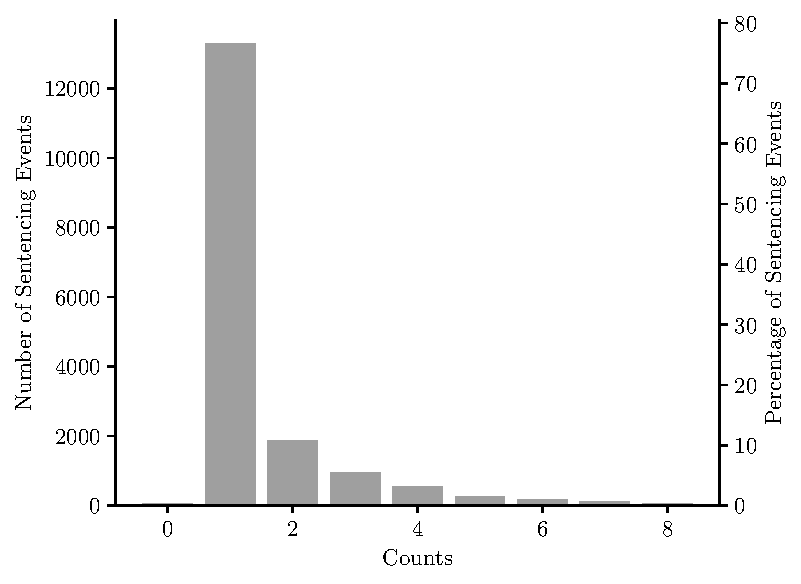
\includegraphics[scale=0.75]{Figures/Count_Histogram}
	\caption{A histogram of the counts.}
	\label{Figure_Hester_Data_Counts_Histogram}
\end{figure}
%
\begin{figure}[h!]
	\centering
	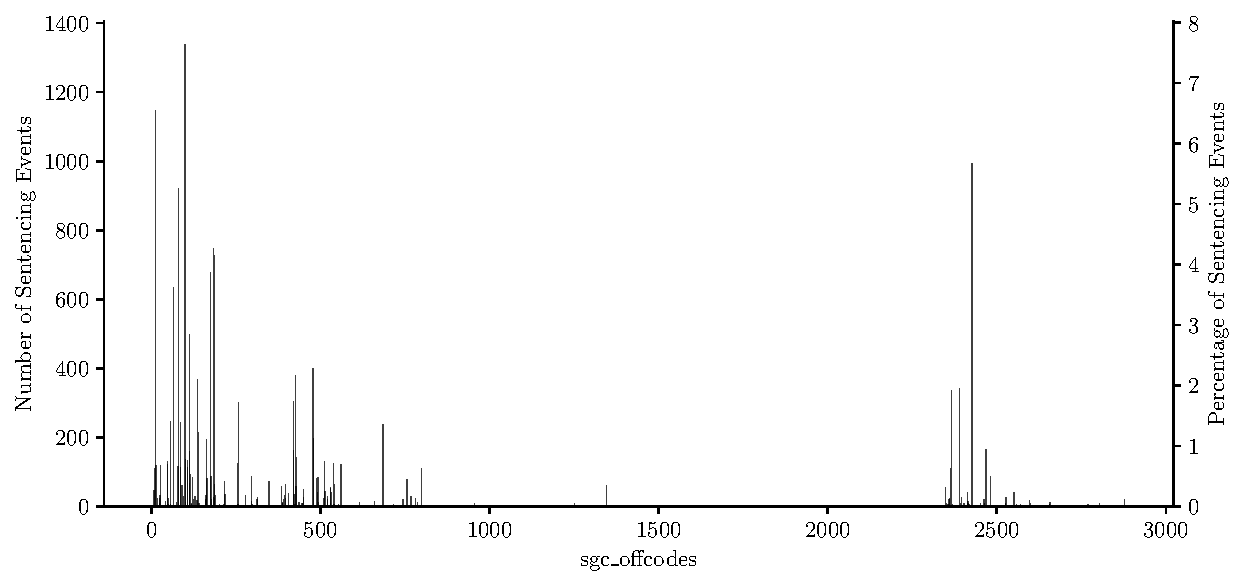
\includegraphics[scale=0.75]{Figures/sgc_offcodes_Histogram}
	\vspace{-2mm}
	\caption{A histogram of sgc\_offcode.}
	\label{Figure_Hester_Data_sgc_offcode_Histogram}
\end{figure}
%
\begin{figure}[h!]
	\centering
	\begin{minipage}{.45\textwidth}
		\centering
		\hspace{-4mm}
		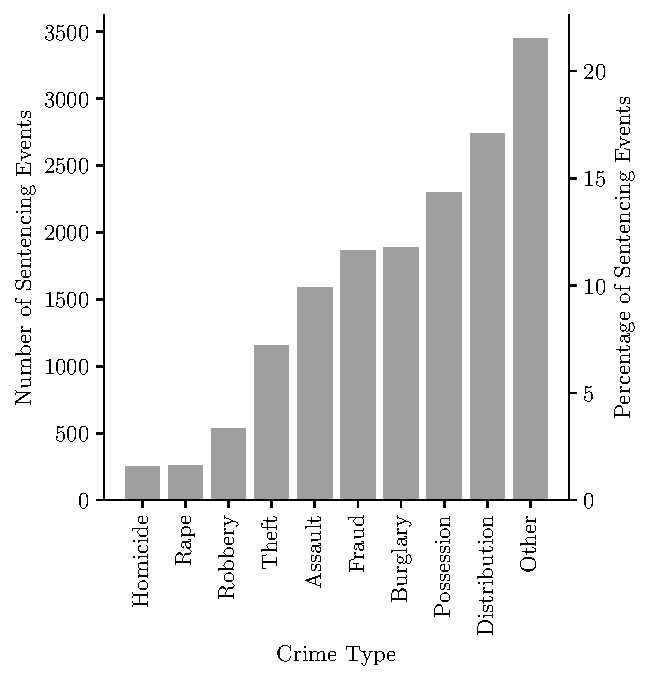
\includegraphics[scale=0.75]{Figures/Crime_Type_Histogram}
		\hspace{4mm}
		\vspace{-6.6mm}
		\caption{A histogram of the crime types.}
		\label{Figure_Hester_Data_Crime_Type_Histogram}
	\end{minipage}
	\hspace{5mm}
	\begin{minipage}{0.45\textwidth}
		\centering
		\hspace{-3mm}
		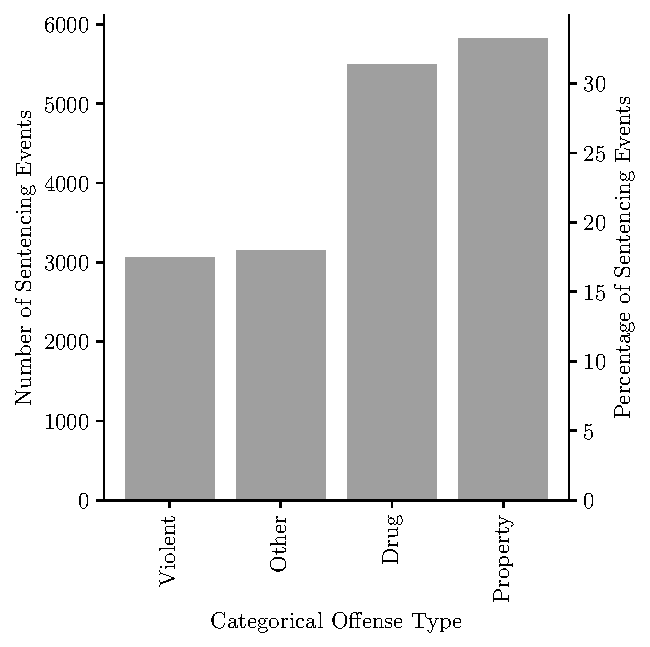
\includegraphics[scale=0.75]{Figures/Categorical_Offense_Type_Histogram}
		\hspace{3mm}
		\vspace{-2mm}
		\caption{A histogram of the offense types.}
		\label{Figure_Hester_Data_Categorical_Offense_Type_Histogram}
	\end{minipage}
\end{figure}
%
\begin{figure}[h!]
	\centering\captionsetup[subfloat]{labelfont=up,font=small}
	\centering
	\hspace*{-8mm}
	\begin{tabular}{cc}
		\subfloat[{\small Drug.}]{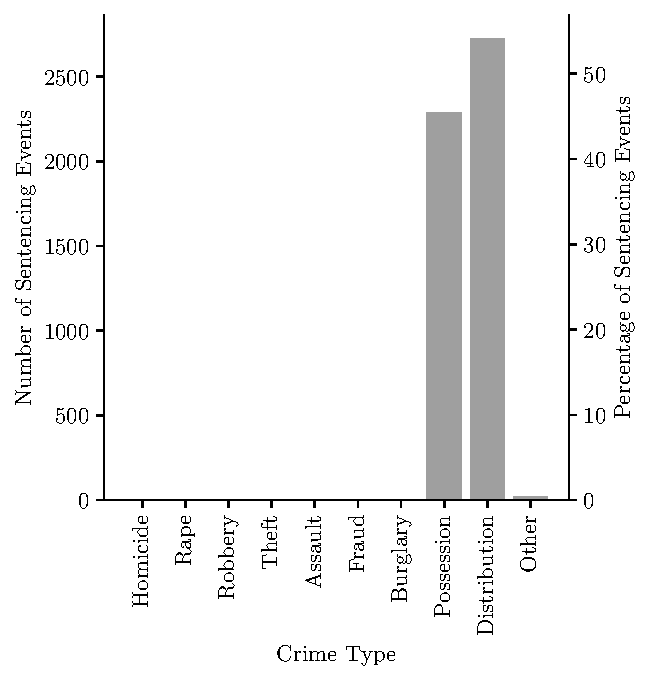
\includegraphics[scale=0.75]{Figures/Drug_Crime_Type_Histogram}}
		&
		\subfloat[{\small Property.}]{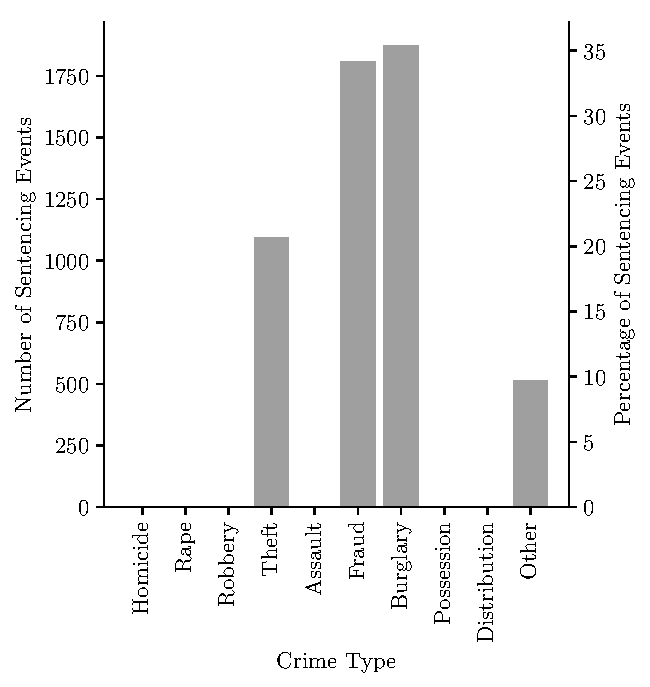
\includegraphics[scale=0.75]{Figures/Property_Crime_Type_Histogram}}
		\\
		\subfloat[{\small Violent.}]{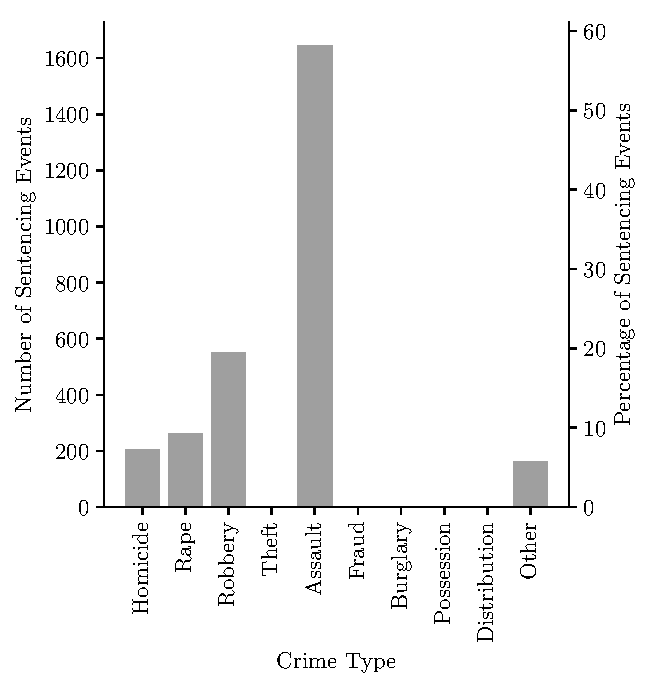
\includegraphics[scale=0.75]{Figures/Violent_Crime_Type_Histogram}}
		&
		\subfloat[{\small Other.}]{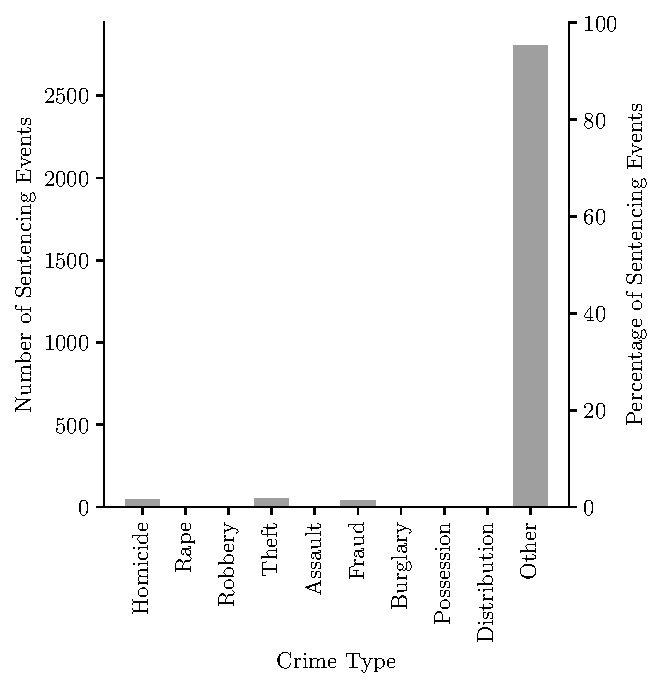
\includegraphics[scale=0.75]{Figures/Other_Crime_Type_Histogram}}
	\end{tabular}
	\caption{A histogram of the crime types for each categorical offense type. This figure is created as follows: Recall that there are four categorical offense types in the offtypeLibHyp data field; see Figure \ref{Figure_Hester_Data_Crime_Type_Histogram}. For each one, we first look for sentencing events that have this categorical offense type. Then, we count how many of these sentencing events fall under each of the 10 crime types depicted in Figure \ref{Figure_Hester_Data_Categorical_Offense_Type_Histogram}, and also see Table \ref{Table_Sentencing_Crime_Type_Data_Fields} for the data fields that provide the crime type information. Repeating this for each of the four offense types Drug, Property, Violent, and Other yields panels (a) through (d) of the figure, respectively.}
	\label{Figure_Hester_Data_offtypeLibHyp}
\end{figure}
%
\begin{figure}[h!]
	\centering
	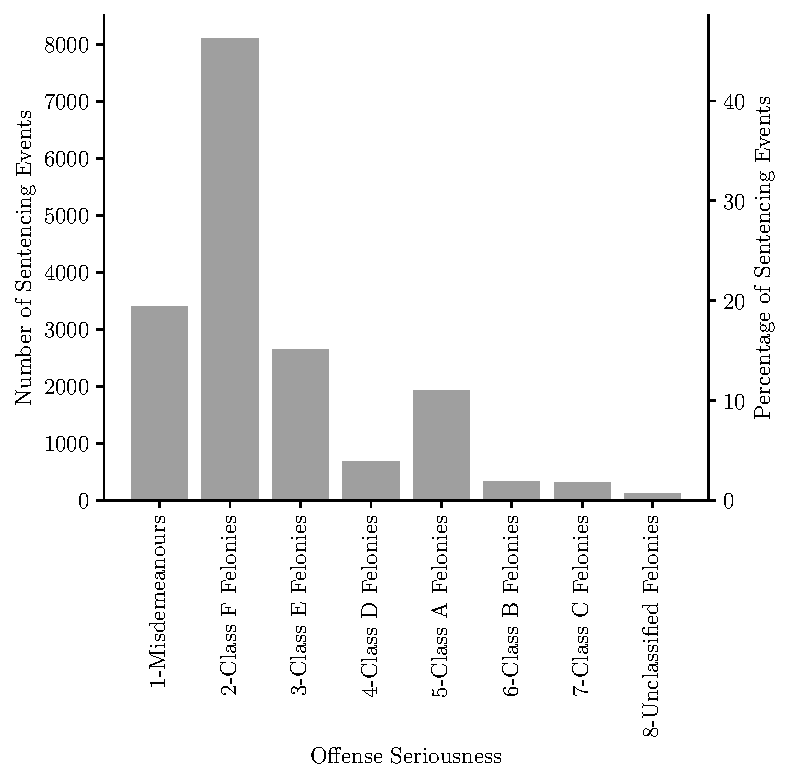
\includegraphics[scale=0.75]{Figures/Offense_Seriousness_Histogram}
	\vspace{-2mm}
	\caption{A histogram of the offense seriousness.}
	\label{Figure_Hester_Data_Offense_Seriousness_Histogram}
\end{figure}
%
\begin{figure}[h!]
	\centering
	\begin{minipage}{.45\textwidth}
		\centering
		\hspace{-4mm}
		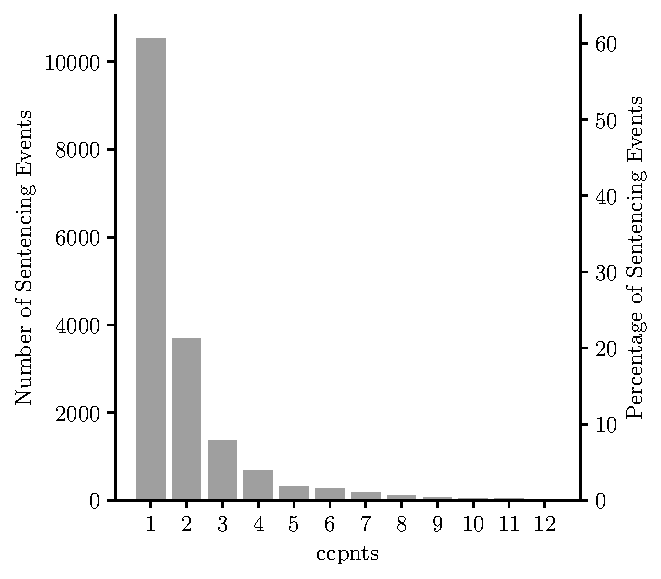
\includegraphics[scale=0.75]{Figures/ccpnts_Histogram}
		\hspace{4mm}
		\vspace{-6.0mm}
		\caption{A histogram of the ccpnts values.}
		\label{Figure_Hester_Data_ccpnts_Histogram}
	\end{minipage}
	\hspace{5mm}
	\begin{minipage}{0.45\textwidth}
		\centering
		\hspace{-3mm}
		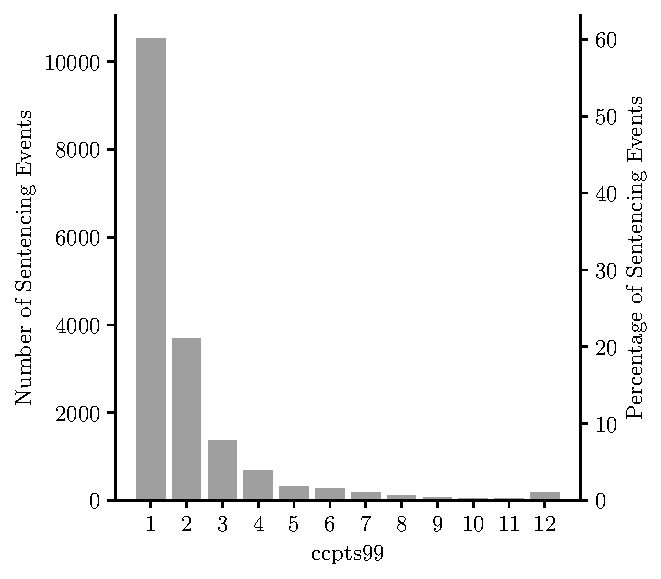
\includegraphics[scale=0.75]{Figures/ccpts99_Histogram}
		\vspace{-6mm}
		\caption{A histogram of the ccpts99 values.}
		\label{Figure_Hester_Data_ccpts99_Histogram}
	\end{minipage}
\end{figure}
%
\begin{figure}[h!]
	\centering
	\begin{minipage}{0.45\textwidth}
		\centering
		\hspace{-4mm}
		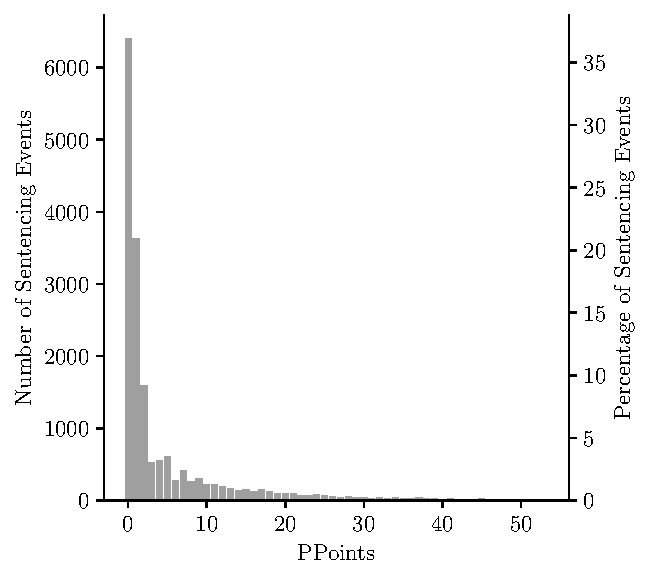
\includegraphics[scale=0.73]{Figures/PPoints_Histogram}
		\hspace{4mm}
		\vspace{-7mm}
		\caption{A histogram of ppoints values.}
		\label{Figure_Hester_Data_PPoints_Histogram}
	\end{minipage}
	\hspace*{5mm}
	\begin{minipage}{0.45\textwidth}
		\centering
		\hspace{-4mm}
		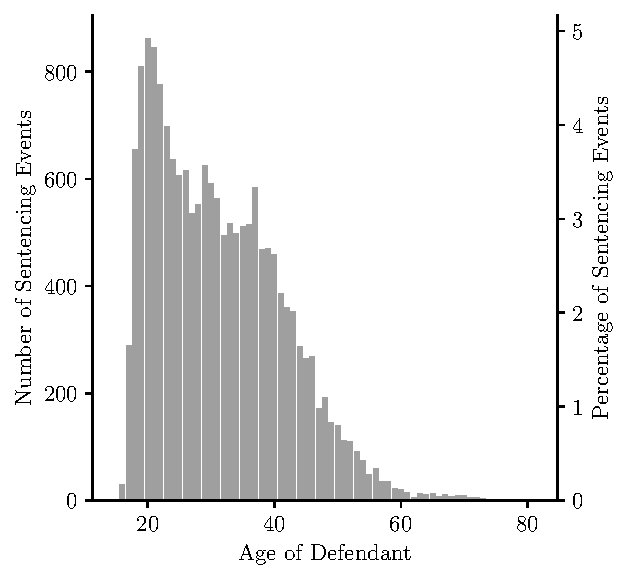
\includegraphics[scale=0.73]{Figures/Ages_Histogram}
		\hspace{4mm}
		\vspace{-7mm}
		\caption{A histogram of the ages of the defendants.}
		\label{Figure_Hester_Data_Age_Histogram}
	\end{minipage}
\end{figure}	
%
\begin{figure}[h!]
	\centering\captionsetup[subfloat]{labelfont=up,font=small}
	\centering
	\hspace*{-8mm}
		\subfloat[{\small Sentence Length.}]{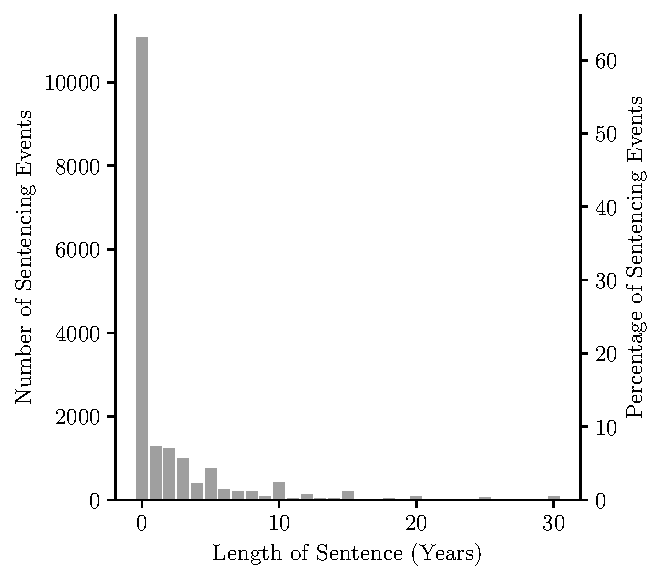
\includegraphics[scale=0.75]{Figures/Sentence_STATA_Histogram}\label{Figure_Hester_Sentence_Length_Histogram}}
		\subfloat[{\small Expected Minimum Sentence.}]{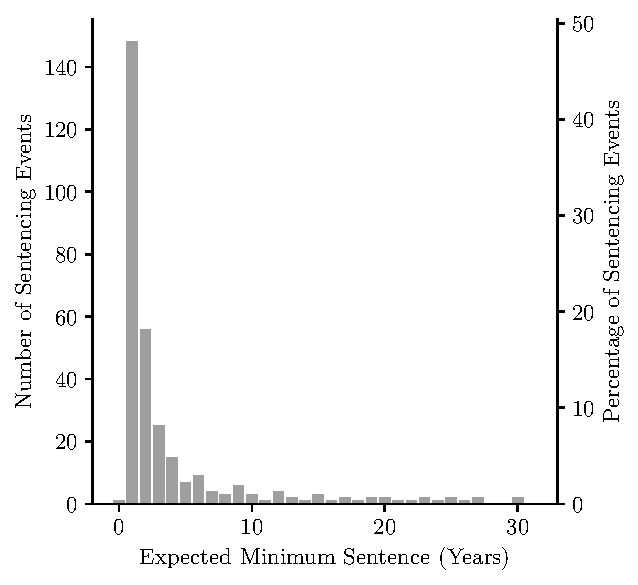
\includegraphics[scale=0.75]{Figures/expmin_Histogram}\label{Figure_Hester_ExpMin_Histogram}}
	\caption{A histogram of the sentence lengths and the expected minimum sentences. The bar at $i$ represents sentencing events with a sentence length or expected minimum sentence between $i-1$ and $i$ years.}
	\label{Figure_Hester_Sentence_And_ExpMin_Histograms}
\end{figure}
%
\begin{figure}[h!]
	\centering\captionsetup[subfloat]{labelfont=up,font=small}
	\centering
	\hspace*{-8mm}
	\subfloat[{\small Sentencing events that end with a trial.}]{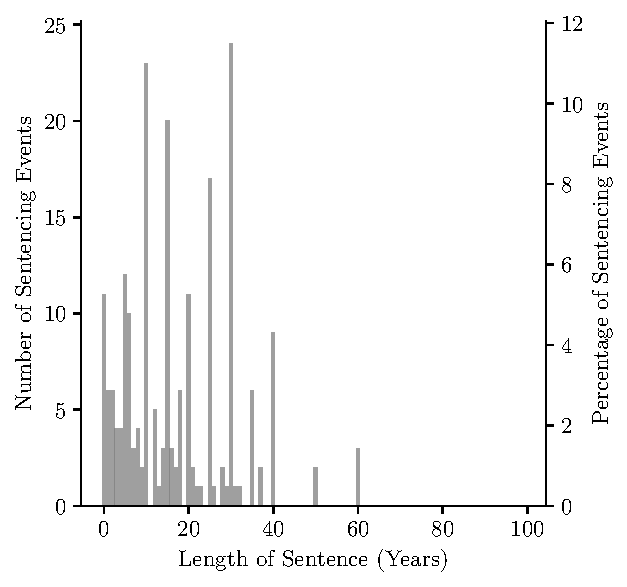
\includegraphics[scale=0.75]{Figures/Sentence_Given_Trial_CSV_Histogram}\label{Figure_Hester_Sentence_Length_Given_Trial_Histogram}}
	\subfloat[{\small Sentencing events that end with a plea.}]{\includegraphics[scale=0.75]{Figures/Sentence_Given_Plea_CSV_Histogram}\label{Figure_Hester_Sentence_Length_Given_Plea_Histogram}}
	\caption{A histogram of the sentence lengths for the sentencing events that end with a trial as well as the sentencing events that end with a plea. The bar at $i$ represents sentencing events with a sentence length between $i-1$ and $i$ years. For visual clarify, in Panel a, all sentencing events with a sentence length greater than or equal to 99 years are combined into one bar, i.e., the bar at 99 years.1 }
	\label{Figure_Hester_Sentence_Length_Given_Trial_And_Plea_Histogram}
\end{figure}
%
\begin{figure}[h!]
	\centering
	\includegraphics[scale=0.75]{Figures/Judge_STATA_Histogram}
	\vspace{-2mm}
	\caption{A histogram of the sentencing judges in the STATA file. The left axis corresponds to the number of sentencing events observed for each judge. The right axis corresponds to the percentage of sentencing events undertaken by each judge.}
	\label{Figure_Hester_Data_STATA_Judge_Histogram}
\end{figure}
%
\begin{figure}[h!]
	\centering\captionsetup[subfloat]{labelfont=up,font=small}
	\centering
	\hspace*{-8mm}
	\subfloat[{\small Perfect Match.}]{\includegraphics[scale=0.7]{Figures/First_Vs_Second_Vs_Third_Best_Match_Perfect}\label{Figure_Mapping_Mismatches_Perfect}}
	\subfloat[{\small Overlapping Match.}]{\includegraphics[scale=0.7]{Figures/First_Vs_Second_Vs_Third_Best_Match_Overlapping}\label{Figure_Mapping_Mismatches_Overlapping}}
	\caption{Weeks of mismatch for the judge name mapped to each judge number. The judge names with the second and third fewest weeks of mismatch are also depicted.}
	\label{Figure_Mapping_Mismatches}
\end{figure}
%
\begin{figure}[h!]
	\centering
	\includegraphics[scale=0.75]{Figures/Mapping_Judge_Numbers_To_Judge_Names_Judge_Distribution}
	\vspace{-2mm}
	\caption{The number of problematic sentencing events for each judge number. The blue bar depicts the number of problematic sentencing events where the schedule of the mapped judge name does not have any county assignments. The red bar depicts the number of problematic sentencing events where the schedule of the mapped judge name has some county assignments, but does not included the county in which the sentencing event occurred.}
	\label{Figure_Mapping_Problematic_Sentencing_Events_Judge_Distribution}
\end{figure}
%
\begin{figure}[h!]
	\centering
	\includegraphics[scale=0.75]{Figures/Mapping_Judge_Numbers_To_Judge_Names_Week_Distribution}
	\vspace{-2mm}
	\caption{The number of problematic sentencing events on each week. The blue bars depict the number of problematic sentencing events where the schedule of the mapped judge name does not have any county assignments. The red bars depict the number of problematic sentencing events where the schedule of the mapped judge name has some county assignments, but does not included the county in which the sentencing event occurred. The grey bars depict the number of problematic sentencing events undertaken by Judge 1 (the fictitious judge).}
	\label{Figure_Mapping_Problematic_Sentencing_Events_Week_Distribution}
\end{figure}

\clearpage

\section{Further Analysis of the Sentencing Events Missing the \emph{date} Data Field}
\label{Sec:Appendix:Missing_Dates}
As discussed in Section \ref{Sec:Sentencing_Data_Description}, about $8.7\%$ of the sentencing events (1551 sentencing events) are missing the \emph{date} data field. This section further analyzes these sentencing events to infer the missing date from the (available) judge and county information.

We start by cleaning the sentencing dataset as described in Appendix \ref{Sec:Appendix:Data_Cleaning}. Then, we fix a sentencing event that is missing the \emph{date} data field. We record the judge number and the county associated with this sentencing event. Next, we use the master calendar (and the mapping from judge numbers to judge names described in Section \ref{Sec:Mapping_Judge_Numbers_To_Judge_Names}) to find the set of weeks on which this judge visited this county. Let us illustrate this through an example: One of the sentencing event missing the \emph{date} date field is undertaken by Judge 4 in Newberry. According to Section \ref{Sec:Mapping_Judge_Numbers_To_Judge_Names}, Judge 4 is Judge Baxley. Judge Baxley visited only Newberry in the week of November 6th 2000. Therefore, the set associated with this sentencing event is \{November 6th 2000\}. We continue this procedure for all sentencing events missing the \emph{data} data field.

Focusing on the sentencing events who are missing the \emph{date} data field, Figure \ref{Figure_Missing_Date_Histogram_of_Potential_Week_Histogram} displays a histogram of the number of visits to the sentencing county by the sentencing judge using his schedule from the master calendar. For example, the first bar indicates that there are 222 sentencing events (missing the \emph{date} data field) that occurred in a county to which the judge was never assigned (according to the master calendar). For 34 out of these 222 sentencing events, the judge visited the circuit court associated with the sentencing event in least one week. For 100 sentencing events, the judge visited the county (associated with this sentencing event) only once. We \emph{assume} these sentencing events occurred during this week. For example, we assume the sentencing event discussed in the previous paragraph occurred in the Week of November 6th 2000. 
%
\begin{note}
	Once the model is finalized, we should discuss whether the week on which a sentence occurred is sufficient for our purposes or an exact date is required. 
\end{note} 

\section{Judge Assignments}
\label{Sec:Appendix:Master_Calendar_Interpretations}
This section provides plausible assignments for the judges by taking advantage of the master calendar and the sentencing dataset. We do not attempt to resolve all cases of conflict. We propose plausible assignments for all judge-week combinations in cases i and ii, but not for all judge-week combinations in cases iii and iv. Also, the fixes we mention are not the only ones that are possible. There are other ways to proceed, too. We do not attempt an exhaustive list of fixes. In that sense, the possible fixes we mention are speculative. Nonetheless, they offer possible ways to address the apparent conflicts between the sentencing dataset and the master calendar.
%
\subsection{Case i - No Assignments.}
%
\begin{plausible_assignment}
	A possible interpretation of the master calendar for the 101 judge-week combinations of Category i for which we do not observe sentencing events (in the sentencing dataset) is as follows: The judge does not have any assignments the entire week.
\end{plausible_assignment}
%
\begin{plausible_assignment}
	A possible interpretation of the master calendar for the 9 judge-week combinations of Category i for which we observe sentencing events, i.e., the judge-week combinations listed in Table \ref{Table_Mater_Calendar_Problematic_Cases_Detailed_Category_i}, is as follows: On the days with sentencing events, the judge is assigned to the county in which he has sentencing events. In the remainder of the week, the judge does not any assignments. For example, in combination 1 of Table \ref{Table_Mater_Calendar_Problematic_Cases_Detailed_Category_i}, Judge 8 is assigned to Dorchester on Monday. He does not have any assignments the rest of the week.
	\label{Plausible_Assignment_Category_i_9Problematic}
\end{plausible_assignment}
%
Plausible Assignment \ref{Plausible_Assignment_Category_i_9Problematic} interprets the 9 judge-week combinations of Category i for which we observe sentencing events as judge-week combinations of Category ii (b).
%
\subsection{Case ii - A Single Assignment}
\subsubsection{Case ii (a)}
%
\begin{plausible_assignment}
	A possible interpretation of the master calendar for the 1872 judge-week combinations of Category ii (a) for which we only observe sentencing events in the county to which the judge is assigned is as follows: The judge is assigned to the assignment on the master calendar the entire week.
\end{plausible_assignment}
%
\begin{plausible_assignment}
	A possible interpretation of the master calendar for the 328 judge-week combinations of Category ii (a) for which we observe sentencing events in a county other than the county to which the judge is assigned is as follows: On days that the judge does not have sentencing events, he is assigned to the assignment on the master calendar. On the days the judge has sentencing events, he is assigned to the counties in which he has sentencing events. For example, in combination 1 of Table \ref{Table_Mater_Calendar_Problematic_Cases_Detailed_Category_iia}, the judge is assigned to Chester on Monday, Wednesday, Thursday, and Friday. He is assigned to York on Tuesday.
\end{plausible_assignment}
%
\subsubsection{Case ii (b)}
\begin{plausible_assignment}
	In judge-week combination 1 of Table \ref{Table_Mater_Calendar_Problematic_Cases_Detailed_Category_iib}, Judge 7 is assigned to Horry on Wednesday, Thursday, and Friday. We observe sentencing events for him in Horry on Tuesday and Friday. A possible assignment for Judge 7 in this week is as follows: The judge does not have any assignments on Monday. He is assigned to Horry the rest of the week.
\end{plausible_assignment}
%
\begin{plausible_assignment}
	In judge-week combinations 2-4 of Table \ref{Table_Mater_Calendar_Problematic_Cases_Detailed_Category_iib}, the judge has a sentencing event in a county other than the county stated on the master calendar. A possible assignment for the judges in these judge-week combinations is as follows: On days that the judge does not have sentencing events, he is assigned to the assignment stated on the master calendar. On the days the judge has sentencing events, he is assigned to the counties in which he has sentencing events. For example, in combination 3 of Table \ref{Table_Mater_Calendar_Problematic_Cases_Detailed_Category_iib}, the judge does not have any assignments on Monday and Tuesday. He is assigned to Barnwell on Wednesday and Friday. He is assigned to both Allendale and Barnwell on Thursday.
\end{plausible_assignment}
%
\subsection{Case iii - Two Assignments}
%
We only propose a plausible assignment for judge-week combination 2 of Table \ref{Table_Mater_Calendar_Problematic_Cases_Detailed_Category_iii_a}. We refrain from providing plausible assignments for the other judge-week combinations of Category iii.
%
\begin{plausible_assignment}
	A possible assignment for Judge 10 in the week of January 8, which corresponds to Judge-week combination 2 of Table \ref{Table_Mater_Calendar_Problematic_Cases_Detailed_Category_iii_a}, is as follows: The judge is assigned to both Florence and Lee on Monday, Tuesday, and Friday. He is assigned to Marion on Wednesday and Thursday.
\end{plausible_assignment}
For now, we refrain from providing plausible interpretations for the remaining judge-week combinations listed in Tables \ref{Table_Mater_Calendar_Problematic_Cases_Detailed_Category_iii_a}-\ref{Table_Mater_Calendar_Problematic_Cases_Detailed_Category_iii_c}.
%
\subsection{Case iv - Multiple Assignments.}
%
\subsubsection{Case iv (a)}
%
There are two judge-week combinations in Category iv (a). We only provide a plausible assignment for the judge-week combination in Table \ref{Table_Mater_Calendar_Problematic_Cases_Detailed_Category_iva}. According to the master calendar, in Combination 1 of Table \ref{Table_Mater_Calendar_Problematic_Cases_Detailed_Category_iva}, Judge 3 is assigned to Aiken, Bamberg, and Barnwell. According to the sentencing dataset, this judge has sentencing events in Aiken on Thursday and in both Bamberg and Barnwell on Monday and Tuesday. Moreover, according to \citet{SCCourts}, the Aiken, Bamberg, and Barnwell courts are less than 46 miles apart. In fact, the Bamberg and Barnwell courts are only 21 miles apart. 
%
\begin{plausible_assignment}
	A possible assignment for Judge 3 in the week of April 30th (judge-week combination 1 of Table \ref{Table_Mater_Calendar_Problematic_Cases_Detailed_Category_iva}) is as follows: The judge is assigned to both Barmberg and Barnwell on Monday and Tuesday. He is assigned to Aiken on Thursday. He is assigned to Bamberg, Barnwell, and Aiken the rest of the week.
\end{plausible_assignment}
%
\subsubsection{Case iv (b)}
%
There are 19 judge-week combinations in Category iv (b). We only provide a plausible assignment for the judge-week combination in Table \ref{Table_Mater_Calendar_Problematic_Cases_Detailed_Category_ivb}.
%
\begin{plausible_assignment}
	A possible assignment for Judge 41 in the week of May 7th, which corresponds to the judge-week combination depicted in Table \ref{Table_Mater_Calendar_Problematic_Cases_Detailed_Category_ivb}, is as follows: Judge 41 is assigned to Spartanburg on Monday. He is assigned to the 13th circuit court on Tuesday. He is in chambers the rest of the week.
\end{plausible_assignment}
%
\subsubsection{Case iv (c)}
%
There are 3 judge-week combinations in Category iv (c). We only provide a plausible assignment for the judge-week combination in Table \ref{Table_Mater_Calendar_Problematic_Cases_Detailed_Category_ivc}.
%
\begin{plausible_assignment}
	A possible assignment for Judge 31 in the week of February 26, which corresponds to the judge-week combination in Table \ref{Table_Mater_Calendar_Problematic_Cases_Detailed_Category_ivc}, is as follows: The judge is assigned to Anderson on Monday, Tuesday, Wednesday, and Thursday. He is assigned to Oconee on Friday.
\end{plausible_assignment}

\end{document}




